% =====================================================================
%  Unit 1 -- Model evaluation
%  (this file is assembled from src/ch01/*.tex by build_chapter.py)
% =====================================================================
\chapter{Model Evaluation}\label{ch:evaluation}

In 2021, a team at the University of Michigan published a retrospective external validation of the then-current
version of a sepsis\index{sepsis prediction} prediction model that was already in use in hundreds of hospitals in the United States. Its
developer reported an area under the ROC curve\index{area under the ROC curve (AUC)}\index{ROC curve} between 0.76 and 0.83; on the 38,455 hospitalisations of their own
hospital, the researchers measured 0.63. At the threshold\index{threshold} they studied, simulated alerts would have flagged about 18\%
of all hospitalisations while missing about two thirds of those with sepsis \citep{wong2021external}. The case shows
why external evaluation under the intended conditions of use is essential: the numbers that had been reported did not
measure what mattered where the model was used.

Training a model is usually the easy part of a machine learning project: modern libraries
fit a random forest\index{random forest} or a neural network in a couple of lines of code. Deciding whether that
model is \emph{good}, whether it is \emph{better} than the alternatives, and whether it is
\emph{good enough} for the purpose it was built for is much harder. Mistakes at this stage
are expensive: a model that looked excellent in the laboratory may lose money, harm people
or silently degrade once it meets real data.

This unit is about \emph{evaluation}: the procedures that give us trustworthy estimates of
how a model will behave on new data, and the metrics that turn that behaviour into numbers
that reflect what we care about. Evaluation is also the backbone of the rest of the course:
we need it to decide how to combine models (Unit~2), to check whether a model is fair or
robust (Unit~3), to automate model building (Unit~4), and to decide when a deployed model
has to be updated (Units~5 and~6).

\begin{objectives}
After studying this unit you should be able to:
\begin{itemize}
  \item explain why the performance on training data\index{training set} is not a reliable estimate, and relate
        underfitting\index{underfitting} and overfitting\index{overfitting} to the bias--variance\index{bias--variance trade-off} decomposition;
  \item design sound evaluation protocols\index{evaluation protocol} (hold-out\index{hold-out}, cross-validation\index{cross-validation}, bootstrap\index{bootstrap}, nested
        cross-validation\index{cross-validation!nested}, group- and time-aware splits) and recognise data leakage\index{data leakage};
  \item compute, interpret and select appropriate metrics to assess classification, regression and unsupervised
        models, and their strengths and weaknesses;
  \item use graphical tools (ROC, precision\index{precision}--recall\index{recall}, lift\index{lift}, reliability diagrams\index{calibration!reliability diagram} and cost
        curves\index{cost curve}) to assess models in different contexts;
  \item distinguish crisp, scoring and probabilistic classifiers and evaluate each of them
        appropriately, including their calibration\index{calibration};
  \item measure performance in imbalanced\index{class imbalance} scenarios and know techniques to address
        imbalanced data sets;
  \item incorporate costs into evaluation and decision making;
  \item evaluate models in specialised settings (conformal prediction\index{conformal prediction}, open-set\index{open-set recognition} recognition,
        computer vision, natural language processing) and compare models statistically.
\end{itemize}
\end{objectives}

% ---------------------------------------------------------------------
\section{Why evaluation matters}\label{sec:why}

\subsection{Evaluation in the data science process}

The Cross-Industry Standard Process for Data Mining, CRISP-DM\index{CRISP-DM} \citep{chapman2000crisp},
describes a data mining project as a cycle of six phases (\cref{fig:crispdm}). Evaluation is
one of them, and it appears \emph{after} modelling and \emph{before} deployment\index{deployment} for a reason.
During modelling, analysts already compare models using technical criteria (``model A is
more accurate than model B''). The evaluation phase asks broader questions: does the model
meet the \emph{business} success criteria defined at the beginning of the project? Was any
important business issue overlooked? Should we deploy, iterate, or start a new project?

\begin{figure}[htbp]
\centering
\begin{tikzpicture}[
  phase/.style={draw=edmnavy,fill=edmnavy!6,rounded corners=3pt,minimum width=29mm,
                minimum height=10mm,align=center,font=\small\sffamily},
  hl/.style={phase,fill=edmbronze!25,draw=edmbronze,very thick},
  arr/.style={-{Stealth[length=2.2mm]},edmnavy,thick},
  back/.style={-{Stealth[length=2mm]},edmnavy!55,dashed}]
  \node[phase] (bu) at (90:3.0)   {Business\\understanding};
  \node[phase] (du) at (30:3.5)   {Data\\understanding};
  \node[phase] (dp) at (-30:3.5)  {Data\\preparation};
  \node[phase] (mo) at (-90:3.0)  {Modelling};
  \node[hl]    (ev) at (-150:3.5) {Evaluation};
  \node[phase] (de) at (150:3.5)  {Deployment};
  \node[draw=edmteal,fill=edmteal!12,cylinder,shape border rotate=90,aspect=0.25,
        minimum width=15mm,minimum height=13mm,font=\small\sffamily] at (0,0) {Data};
  \draw[arr] (bu) -- (du);
  \draw[back] (du.north west) to[bend right=18] (bu.east);
  \draw[arr] (du) -- (dp);
  \draw[arr] (dp) -- (mo);
  \draw[back] (mo.east) to[bend right=18] (dp.south west);
  \draw[arr] (mo) -- (ev);
  \draw[arr] (ev) -- (de);
  \draw[back] (ev.north east) to[out=60,in=215] (bu.south west);
\end{tikzpicture}
\caption{The CRISP-DM process model \citep{chapman2000crisp}. Evaluation (highlighted) checks
the models against the business objectives before deciding on deployment; the dashed arrows
show the most frequent iterations.}
\label{fig:crispdm}
\end{figure}

Twenty years after CRISP-DM was proposed, \citet{martinezplumed2021crisp} analysed how data science
projects are actually carried out and found that they follow more flexible
\emph{trajectories}: some projects are exploratory, some start from the data rather than
from a business goal, and many go back and forth between activities. Evaluation, however,
remains present in all of them, and its role grows as models are deployed in more varied
and changing contexts.

\subsection{What exactly are we evaluating?}

The word ``evaluation'' hides at least three different objects:
\begin{enumerate}
  \item a \emph{trained model} $h$, a concrete artefact that we may deploy
        (\emph{model assessment}: how well will \emph{this} model perform?);
  \item a \emph{learning procedure} (an algorithm together with its preprocessing and
        hyperparameter tuning\index{hyperparameter optimisation}), which produces models from data (\emph{algorithm comparison}:
        is random forest a better choice than logistic regression\index{logistic regression} for this kind of data?);
  \item a \emph{decision system}, which uses the model's outputs to act in a given context:
        thresholds, costs, capacity constraints (is the system good enough to be deployed?).
\end{enumerate}
Each question needs three ingredients: a \emph{metric} aligned with the purpose of the model,
an \emph{estimation protocol} that produces an honest estimate of that metric, and a
statement of the \emph{uncertainty} of the estimate.

The purpose of the model is described by its \emph{operating context}: the class distribution
in deployment, the costs of the different errors, the fraction of cases that can be acted
upon, the data distribution itself. Two models can be ranked differently in two contexts,
and the context may change after deployment. Evaluating models over ranges of contexts,
rather than at a single point, is one of the themes of this unit
\citep{hernandez2012unified}; detecting when the context has changed is one of the themes of
Unit~6 \citep{morenotorres2012unifying}.

\begin{keyidea}
A metric is a model of what we care about. Before computing any number, make explicit what
the model will be used for, which errors matter and how much, and under which conditions it
will operate.
\end{keyidea}

\subsection{Notation}

\Cref{tab:notation} summarises the notation used in this unit.

\begin{table}[htbp]
\centering\small
\caption{Notation used in this unit.}\label{tab:notation}
\begin{tabularx}{\textwidth}{@{}lX@{}}
\toprule
Symbol & Meaning\\
\midrule
$(x_i,y_i)$, $i=1,\dots,n$ & examples: input $x_i$ and actual output $y_i$ (also written $f(x_i)$)\\
$S$ & a set of (test) examples, with $n=|S|$\\
$h$ & a model (hypothesis); $h(x)=\hat y$ is its prediction\\
$c$ & number of classes\\
$P$, $N$ & number of actual positive and negative examples\\
$\TP$, $\FP$, $\TN$, $\FN$ & true positives, false positives, true negatives, false negatives\\
$s(x)$ & score given by a scoring classifier (higher means ``more positive'')\\
$\hat p(x)$, $p(i,j)$ & estimated probability of the positive class / of example $i$ belonging to class $j$\\
$f(i,j)$ & $1$ if example $i$ belongs to class $j$ and $0$ otherwise\\
$c_{\mathrm{FP}}$, $c_{\mathrm{FN}}$ & cost of a false positive / of a false negative\\
$\pi_+$, $\pi_-$ & proportion of positive and negative examples (prevalence)\\
\bottomrule
\end{tabularx}
\end{table}

% ---------------------------------------------------------------------
\section{Generalisation, overfitting and the bias--variance trade-off}\label{sec:biasvariance}

Let the examples $(x,y)$ be drawn independently from an unknown distribution $\mathcal D$ and
let $\ell(y,\hat y)$ be a loss function (for instance the 0--1 loss in classification or the
squared error in regression). What we would like to know is the \emph{true risk} (or
generalisation\index{generalisation} error) of a model,
\begin{equation}
  R(h)=\E_{(x,y)\sim\mathcal D}\bigl[\ell\bigl(y,h(x)\bigr)\bigr],
\end{equation}
but we can only compute averages over finite samples, such as the \emph{training error}
\begin{equation}
  \widehat R_{\text{train}}(h)=\frac1n\sum_{i=1}^n \ell\bigl(y_i,h(x_i)\bigr).
\end{equation}
Because the learning algorithm chose $h$ precisely to make $\widehat R_{\text{train}}$ small,
the training error is an \emph{optimistically biased} estimate of $R(h)$. This simple fact is
the reason why evaluation needs data that played no role in building the model.

\subsection{The papaya problem}

\citet{shalev2014understanding} illustrate the problem with a story. Imagine arriving on an
island where papayas are a common food. You want to learn to predict whether a papaya is
tasty from two features you can observe at the market: its softness and its colour. You buy
a few papayas, taste them, and record the results.

A first learner simply memorises: it predicts ``tasty'' for papayas identical to the tasty
ones in the sample and ``not tasty'' for everything else. Its training error is zero, but it
is useless, since almost every new papaya differs slightly from those already tasted. This
is \emph{overfitting\index{overfitting|textbf}}: the model fits the particular sample, including its noise, instead of
the underlying regularity.

A second learner assumes that tasty papayas are those whose softness and colour both lie in
some intermediate range, so that it only has to find an axis-parallel rectangle. This
\emph{inductive bias\index{inductive bias|textbf}} prevents memorisation and lets the learner generalise. But if the
assumptions are too strong (say, ``a papaya is tasty if its colour exceeds a threshold'', or
``a papaya is tasty if it is close to the average tasty papaya''), the model cannot
represent the real concept and errs systematically, on the training data as well as on new
data. This is \emph{underfitting\index{underfitting|textbf}}.

\subsection{The bias--variance decomposition}

For regression with squared loss the trade-off can be made exact. Assume
$y=f(x)+\varepsilon$, with $\E[\varepsilon]=0$ and $\Var(\varepsilon)=\sigma^2$, and let
$h_D$ be the model learned from a random training set $D$. Write
$\bar h(x)=\E_D[h_D(x)]$ for the average prediction over training sets. For a fixed input
$x_0$, adding and subtracting $f(x_0)$ and $\bar h(x_0)$ and noticing that the cross terms
have zero expectation gives
\begin{equation}\label{eq:biasvariance}
  \E_{D,\varepsilon}\bigl[(y-h_D(x_0))^2\bigr]
  = \underbrace{\sigma^2}_{\text{noise}}
  + \underbrace{\bigl(f(x_0)-\bar h(x_0)\bigr)^2}_{\text{bias}^2}
  + \underbrace{\E_D\bigl[(h_D(x_0)-\bar h(x_0))^2\bigr]}_{\text{variance}}.
\end{equation}
The three terms have a clear interpretation:
\begin{itemize}
  \item the \emph{noise} $\sigma^2$ is irreducible: no model can predict the random part of $y$;
  \item the \emph{bias} measures the error due to wrong or too restrictive assumptions of the
        learning algorithm. High bias means that the model pays little attention to the
        data and oversimplifies the problem: \emph{underfitting\index{underfitting|textbf}};
  \item the \emph{variance} measures how much the model changes when the training set
        changes. High variance means that the model is sensitive to small fluctuations of the
        sample and fits its noise: \emph{overfitting\index{overfitting|textbf}}.
\end{itemize}

\Cref{fig:polyfits} fits polynomials of increasing degree to 20 noisy points of
$f(x)=\sin(2\pi x)$. The straight line underfits (training and test MSE\index{mean squared error (MSE)} of $0.203$ and
$0.236$); the degree-4 polynomial captures the shape (0.069 and 0.074); the degree-15
polynomial passes very close to every training point (training MSE 0.016) but oscillates
wildly between them, and its test MSE explodes to about $3\times10^3$.

\begin{figure}[htbp]
\centering
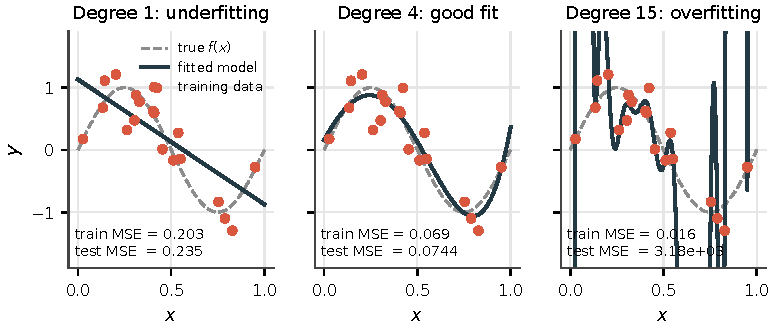
\includegraphics[width=\textwidth]{ch01/polyfits}
\caption{Underfitting and overfitting. Polynomials of degree 1, 4 and 15 fitted to the same
20 noisy observations of $\sin(2\pi x)$. The test error is computed on 5000 new points drawn
from the same range.}
\label{fig:polyfits}
\end{figure}

To see the decomposition at work, \cref{fig:biasvariance} repeats the experiment 500 times
with the same 40 input positions and fresh noise each time, and estimates each term of
\cref{eq:biasvariance}. As the degree grows, the bias drops quickly (from 0.54 for a
constant model to practically zero from degree~5 on), while the variance grows steadily
(from 0.002 to 0.061). The expected test error, which is their sum plus the noise, is
U-shaped, with its minimum at degree~3. The training error, in contrast, keeps decreasing:
it is blind to overfitting.

\begin{figure}[htbp]
\centering
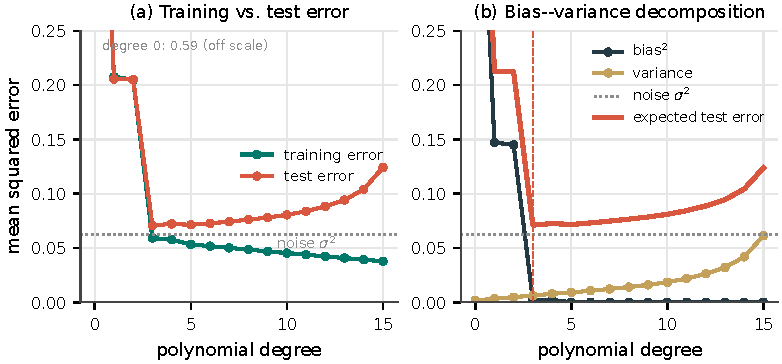
\includegraphics[width=\textwidth]{ch01/bias_variance}
\caption{(a) Training error decreases monotonically with model complexity, while test error
first decreases and then increases. (b) Bias--variance decomposition estimated by simulation
(500 training sets); the dashed line marks the complexity with the lowest expected error.}
\label{fig:biasvariance}
\end{figure}

For the 0--1 loss of classification the decomposition is not additive in the same simple way
\citep{domingos2000unified}, but the intuition carries over: flexible models have low bias and
high variance, rigid models the opposite \citep{geman1992neural}.

\subsection{Complexity in practice: the \texorpdfstring{$k$}{k}-nearest neighbours example}

The complexity of a model is controlled by its hyperparameters: the degree of a polynomial,
the depth of a tree, the strength of a regularisation term, the number of boosting\index{boosting}
iterations, or the number of neighbours $k$ in $k$-NN. \Cref{fig:knn} shows $k$-NN on a
two-moons problem. With $k=1$ every training point is classified correctly (training accuracy\index{accuracy}
1.00) but the frontier is jagged and the test accuracy is only 0.88; with $k=150$ the frontier
is almost a straight line and both accuracies are low (0.82 and 0.83); $k=15$ is a good
compromise (0.94 and 0.92). Choosing a hyperparameter is choosing a point on the bias--variance\index{bias--variance trade-off}
trade-off, and this choice requires data that are not used for training
(\cref{sec:protocols}).

\begin{figure}[htbp]
\centering
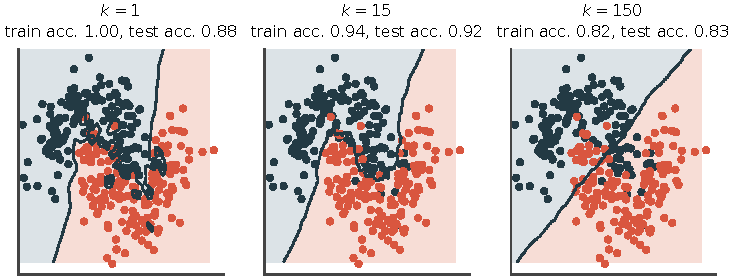
\includegraphics[width=\textwidth]{ch01/knn_boundaries}
\caption{Decision regions of $k$-NN on 300 training examples for three values of $k$. Small
$k$ means high variance (overfitting); large $k$ means high bias (underfitting).}
\label{fig:knn}
\end{figure}

\subsection{Learning curves}

A \emph{learning curve\index{learning curve|textbf}} plots the training and validation performance as a function of the
size of the training set (\cref{fig:learningcurves}). It is a simple and powerful diagnostic:
\begin{itemize}
  \item \emph{high bias}: both curves converge quickly to a similar, unsatisfactory value
        (logistic regression on the two moons, about 0.86). More data will not help; we need
        a more flexible model or better features;
  \item \emph{high variance}: there is a persistent gap between the training curve (1.00 for
        an unpruned tree) and the validation curve (0.88). More data, regularisation or
        ensembles\index{ensemble} (Unit~2) will help;
  \item a good compromise shows both curves close and high ($k$-NN with $k=25$: 0.92 and 0.91).
\end{itemize}

\begin{figure}[htbp]
\centering
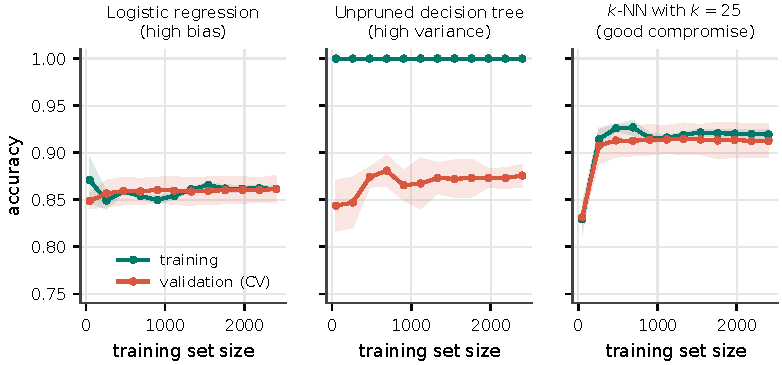
\includegraphics[width=\textwidth]{ch01/learning_curves}
\caption{Learning curves (mean and standard deviation over 5 folds) for three models on the
two-moons problem with 3000 examples.}
\label{fig:learningcurves}
\end{figure}

\begin{further}
The U-shaped curve of \cref{fig:biasvariance} is not the whole story for heavily
over-parameterised models such as deep neural networks. \citet{belkin2019reconciling}
documented a \emph{double descent}: beyond the point where the model can interpolate the
training data, the test error may decrease again as the number of parameters keeps growing.
For the models used in most tabular data science problems, the classical picture remains a
reliable guide.
\end{further}

% ---------------------------------------------------------------------
\section{Estimating performance: evaluation protocols}\label{sec:protocols}

The golden rule of evaluation is simple to state and easy to break: \emph{the performance of
a model must be estimated on data that played no role in building it}, and ``building''
includes preprocessing, feature selection, hyperparameter tuning\index{hyperparameter optimisation} and model selection.

\subsection{Training, validation and test data}

It is useful to separate two activities \citep[Chapter~7]{hastie2009elements}:
\emph{model selection}, which chooses among models or hyperparameters, and
\emph{model assessment}, which estimates the performance of the final choice. With enough
data, the cleanest approach uses three disjoint sets: a \emph{training set\index{training set|textbf}} to fit the
models, a \emph{validation set\index{validation set|textbf}} to choose among them, and a \emph{test set\index{test set|textbf}}, used once, to
assess the chosen model. If the test set is used repeatedly to take decisions, it silently
becomes a validation set and its estimates become optimistic; leaderboards of public
competitions show this effect regularly.

\subsection{Hold-out estimation}

The simplest protocol randomly splits the data into a training and a test set, typically
with 20--30\% of the data for testing. In classification the split should be
\emph{stratified\index{cross-validation!stratified|textbf}}, so that both parts keep the class proportions. The hold-out\index{hold-out} estimate is
cheap but has two drawbacks: the model is trained on less data than available, and the
estimate has high variance, because it depends on a single test sample. If a classifier with
true accuracy 0.85 is tested on 200 examples, the number of correct predictions is binomial,
the standard error of the accuracy is $\sqrt{0.85\cdot0.15/200}\approx0.025$, and an
approximate 95\% interval spans about $\pm0.05$. Differences of one or two points between
models tested this way mean very little (\cref{sec:stats}).

\subsection{Cross-validation}

In \emph{$k$-fold cross-validation\index{cross-validation|textbf}} (CV) the data are partitioned into $k$ folds
$F_1,\dots,F_k$ of similar size. Each fold is used once as test set while the model is
trained on the remaining $k-1$ folds (\cref{fig:cvschemes}a), and the estimate pools all the
test predictions:
\begin{equation}
  \widehat{R}_{\text{CV}}=\frac1n\sum_{j=1}^{k}\sum_{i\in F_j}\ell\bigl(y_i,h^{(-j)}(x_i)\bigr),
\end{equation}
where $h^{(-j)}$ is the model trained without fold $F_j$. Every example is used for testing
exactly once, and every model is trained on a fraction $(k-1)/k$ of the data. Some practical
points:
\begin{itemize}
  \item values of $k=5$ or $k=10$, with stratification, are a good compromise between bias
        and variance \citep{kohavi1995study};
  \item \emph{leave-one-out} CV ($k=n$) is almost unbiased but expensive and has high
        variance; \emph{repeated} CV, with several random partitions, reduces the variance
        due to the particular partition;
  \item CV estimates the performance of the \emph{learning procedure} when trained on
        $(k-1)n/k$ examples, not of a particular model. After CV, the final model is retrained
        on all the data, so the estimate is slightly pessimistic;
  \item the fold estimates are not independent (the training sets overlap), and there is no
        unbiased estimator of the variance of the CV estimate \citep{bengio2004no}. This has
        consequences for statistical tests (\cref{sec:stats}). \citet{arlot2010survey} review
        the theory.
\end{itemize}

\begin{figure}[htbp]
\centering
\begin{subfigure}[b]{0.49\textwidth}
\centering
\begin{tikzpicture}[x=9.5mm,y=5.5mm,font=\scriptsize\sffamily]
  \foreach \c in {1,...,5} \node at (\c-0.5,0.55) {Fold \c};
  \foreach \r in {1,...,5}{
    \node[anchor=east] at (-0.1,-\r+0.5) {Iteration \r};
    \foreach \c in {1,...,5}{
      \ifnum\c=\r
        \filldraw[fill=edmcoral!85,draw=white,thick] (\c-1,-\r) rectangle (\c,-\r+1);
      \else
        \filldraw[fill=edmnavy!18,draw=white,thick] (\c-1,-\r) rectangle (\c,-\r+1);
      \fi
    }
  }
\end{tikzpicture}
\caption{5-fold cross-validation}
\end{subfigure}\hfill
\begin{subfigure}[b]{0.49\textwidth}
\centering
\begin{tikzpicture}[x=4.4mm,y=5.5mm,font=\scriptsize\sffamily]
  \foreach \r in {1,...,4}{
    \node[anchor=east] at (-0.2,-\r+0.5) {Split \r};
    \pgfmathtruncatemacro{\ntr}{4+2*(\r-1)}
    \pgfmathtruncatemacro{\nte}{\ntr+2}
    \foreach \t in {0,...,11}{
      \ifnum\t<\ntr
        \filldraw[fill=edmnavy!18,draw=white,thick] (\t,-\r) rectangle (\t+1,-\r+1);
      \else\ifnum\t<\nte
        \filldraw[fill=edmcoral!85,draw=white,thick] (\t,-\r) rectangle (\t+1,-\r+1);
      \else
        \filldraw[fill=black!6,draw=white,thick] (\t,-\r) rectangle (\t+1,-\r+1);
      \fi\fi
    }
  }
  \draw[-{Stealth},thick,edmnavy] (0,-4.5) -- (12.4,-4.5) node[right] {time};
\end{tikzpicture}
\caption{Forward chaining for time series}
\end{subfigure}
\caption{Two evaluation schemes. Light blue: training data; red: test data; grey: data not
used in that split. In (b) the model is always tested on data that come after the training
period, as it will be in deployment (compare with \cref{lst:timeseries}).}
\label{fig:cvschemes}
\end{figure}

\subsection{The bootstrap}

A bootstrap\index{bootstrap} sample is obtained by drawing $n$ examples \emph{with replacement} from the data
set. The probability that a given example is never drawn is $(1-1/n)^n\approx e^{-1}\approx
0.368$, so each bootstrap sample contains about 63.2\% of the distinct examples, and the
remaining \emph{out-of-bag\index{out-of-bag estimate|textbf}} (OOB) examples can be used for testing. Repeating the process $B$
times and averaging the OOB errors gives a pessimistic estimate (each model sees only 63.2\%
of the distinct examples); the \emph{.632 estimator} corrects it by mixing it with the
optimistic training error,
\begin{equation}
  \widehat R_{.632}=0.368\,\widehat R_{\text{train}}+0.632\,\widehat R_{\text{OOB}},
\end{equation}
and the \emph{.632+} variant further corrects the case of strongly overfitting models
\citep{efron1997improvements}. The bootstrap is also the standard tool to build confidence
intervals\index{confidence interval} for any metric (\cref{sec:stats}), and the OOB idea is used by random forests
(Unit~2).

\subsection{Model selection and nested cross-validation}

Hyperparameters are usually tuned by evaluating many candidate configurations with
cross-validation and keeping the best one. The CV score of the winner, however, is
optimistically biased: when many candidates are compared on the same data, the best one is
partly the luckiest one \citep{varma2006bias,cawley2010over}. To estimate the performance of
the whole procedure (``tune with grid search\index{grid search}, then train''), the tuning must itself be
evaluated inside an outer CV loop. This is \emph{nested cross-validation\index{cross-validation!nested|textbf}\index{cross-validation|textbf}}
(\cref{alg:nestedcv}).

\begin{algorithm}[htbp]
\caption{Nested cross-validation}\label{alg:nestedcv}
\begin{algorithmic}[1]
\Require data $D$; learning procedure $\mathcal A_\theta$ with hyperparameters
         $\theta\in\Theta$; numbers of outer and inner folds $K$ and $J$
\State split $D$ into outer folds $F_1,\dots,F_K$
\For{$k=1,\dots,K$}
  \State $D_{\text{tr}}\gets D\setminus F_k$
  \For{each $\theta\in\Theta$} \Comment{inner loop: model selection}
    \State $\text{score}(\theta)\gets$ $J$-fold CV estimate of $\mathcal A_\theta$ on $D_{\text{tr}}$
  \EndFor
  \State $\theta_k^\star\gets\argmax_\theta\ \text{score}(\theta)$
  \State $h_k\gets\mathcal A_{\theta_k^\star}(D_{\text{tr}})$ \Comment{refit on the outer training data}
  \State $e_k\gets$ performance of $h_k$ on $F_k$ \Comment{outer loop: assessment}
\EndFor
\State \Return $\frac1K\sum_{k}e_k$ \Comment{estimate for the \emph{whole} tuning procedure}
\end{algorithmic}
\end{algorithm}

\Cref{lst:nested} tunes an SVM over 30 hyperparameter combinations on a small, noisy problem.
The inner-CV AUC of the selected configuration is 0.782, but the honest nested estimate is
0.746: an optimism of almost four points of AUC, larger than many of the differences between
models reported in practice. Note that nested CV evaluates the tuning \emph{procedure}; the
model finally deployed is obtained by running that procedure on all the data.

\begin{pylisting}[label={lst:nested}]{Optimistic bias of the best inner-CV score and nested cross-validation}
from sklearn.datasets import make_classification
from sklearn.model_selection import GridSearchCV, StratifiedKFold, cross_val_score
from sklearn.pipeline import make_pipeline
from sklearn.preprocessing import StandardScaler
from sklearn.svm import SVC

# A small, noisy problem: 150 examples, 40 features (only 4 informative)
X, y = make_classification(n_samples=150, n_features=40, n_informative=4,
                           flip_y=0.15, class_sep=0.8, random_state=2)
inner = StratifiedKFold(5, shuffle=True, random_state=1)
outer = StratifiedKFold(5, shuffle=True, random_state=2)
grid = {"svc__C": [0.01, 0.1, 1, 10, 100, 1000],
        "svc__gamma": [1e-4, 1e-3, 1e-2, 1e-1, 1]}          # 30 candidate models
search = GridSearchCV(make_pipeline(StandardScaler(), SVC()), grid,
                      cv=inner, scoring="roc_auc")

search.fit(X, y)                     # model selection using all the data
print(f"Selected: {search.best_params_}")
print(f"Inner-CV AUC of the selected model (optimistic): {search.best_score_:.4f}")
# Nested CV: the WHOLE tuning procedure is repeated inside each outer fold
nested = cross_val_score(search, X, y, cv=outer, scoring="roc_auc")
print(f"Nested CV AUC (honest): {nested.mean():.4f} +/- {nested.std():.4f}")
\end{pylisting}
\begin{pyoutput}
Selected: {'svc__C': 1, 'svc__gamma': 0.01}
Inner-CV AUC of the selected model (optimistic): 0.7822
Nested CV AUC (honest): 0.7458 +/- 0.0257
\end{pyoutput}

\subsection{Dependent data: groups and time}

Random splits assume that examples are independent. When they are not, random CV is
optimistic, because information leaks between related training and test examples:
\begin{itemize}
  \item \emph{grouped data}: several examples come from the same patient, customer, device
        or session. All the examples of a group must fall on the same side of each split
        (\code{GroupKFold} in scikit-learn); otherwise the model is tested on ``people'' it
        has already seen;
  \item \emph{temporal data}: the model will always predict the future from the past, so it
        must be evaluated the same way, training on an initial period and testing on the
        following one (\emph{forward chaining} or \emph{rolling-origin} evaluation,
        \cref{fig:cvschemes}b and \cref{lst:timeseries}). A gap between training and test
        periods avoids leakage\index{data leakage} through autocorrelation. \citet{bergmeir2012use} discuss when
        standard CV is still acceptable for time series;
  \item \emph{spatial data}: nearby locations are similar, and blocked spatial CV is
        needed \citep{roberts2017cross}.
\end{itemize}

\begin{pylisting}[label={lst:timeseries}]{Forward-chaining splits for 12 consecutive time steps}
import numpy as np
from sklearn.model_selection import TimeSeriesSplit

X = np.arange(12).reshape(-1, 1)          # 12 consecutive time steps
for k, (tr, te) in enumerate(TimeSeriesSplit(n_splits=4, test_size=2).split(X), 1):
    print(f"fold {k}: train={tr.tolist()}  test={te.tolist()}")
\end{pylisting}
\begin{pyoutput}
fold 1: train=[0, 1, 2, 3]  test=[4, 5]
fold 2: train=[0, 1, 2, 3, 4, 5]  test=[6, 7]
fold 3: train=[0, 1, 2, 3, 4, 5, 6, 7]  test=[8, 9]
fold 4: train=[0, 1, 2, 3, 4, 5, 6, 7, 8, 9]  test=[10, 11]
\end{pyoutput}

\subsection{Data leakage}

\emph{Data leakage\index{data leakage|textbf}} is the use, during training or evaluation, of information that would not
be available when the model is used in practice \citep{kaufman2012leakage}. It is the most
common cause of results that look too good to be true. Typical forms are:
\begin{itemize}
  \item \emph{target leakage}: features that are consequences of the target or are recorded
        after the event (the number of days in hospital to predict hospital admission, or a
        late-payment fee to predict default);
  \item \emph{train--test contamination\index{contamination of benchmarks|textbf}}: preprocessing steps (scaling, imputation, feature
        selection, resampling, target encoding) fitted on the whole data set before
        splitting it;
  \item \emph{temporal leakage}: random splits of time-ordered data, or features computed
        with future information;
  \item \emph{duplicates}: identical or near-identical examples (the same patient, the same
        product photographed twice, augmented copies) on both sides of a split.
\end{itemize}
\Cref{lst:leakage} reproduces a classic experiment \citep[Section~7.10.2]{hastie2009elements}.
With 5000 pure-noise features and random labels, any honest estimate of accuracy must be
close to 0.5. Selecting the 20 features most correlated with the labels \emph{before}
cross-validation produces an estimated accuracy of 0.87; doing the selection inside each fold
gives the correct 0.50. \citet{kapoor2023leakage} found leakage of this kind in hundreds of
published studies across many scientific fields.

\begin{pylisting}[label={lst:leakage}]{Feature selection outside versus inside cross-validation}
import numpy as np
from sklearn.feature_selection import SelectKBest, f_classif
from sklearn.linear_model import LogisticRegression
from sklearn.model_selection import StratifiedKFold, cross_val_score
from sklearn.pipeline import make_pipeline

rng = np.random.default_rng(0)
X = rng.normal(size=(100, 5000))    # 5000 pure-noise features
y = rng.integers(0, 2, size=100)    # random labels: true accuracy is 0.5
cv = StratifiedKFold(n_splits=5, shuffle=True, random_state=0)
clf = LogisticRegression(max_iter=1000)

# WRONG: the features are selected looking at ALL the labels, then we do CV
X_sel = SelectKBest(f_classif, k=20).fit_transform(X, y)
wrong = cross_val_score(clf, X_sel, y, cv=cv)

# RIGHT: selection is part of the model, so it is refitted inside each fold
right = cross_val_score(make_pipeline(SelectKBest(f_classif, k=20), clf), X, y, cv=cv)
print(f"Wrong CV accuracy: {wrong.mean():.2f}")
print(f"Right CV accuracy: {right.mean():.2f}")
\end{pylisting}
\begin{pyoutput}
Wrong CV accuracy: 0.87
Right CV accuracy: 0.50
\end{pyoutput}

\begin{pitfall}
Any step that looks at the data (including the labels) is part of the model. Put scaling,
imputation, feature selection, resampling and encoders inside a \code{Pipeline}, and evaluate
the pipeline, never a model fitted on preprocessed data.
\end{pitfall}

% ---------------------------------------------------------------------
\section{Evaluating crisp classifiers}\label{sec:crisp}

A \emph{crisp} classifier outputs a class label, $h:\mathcal X\to\{1,\dots,c\}$. Scoring and
probabilistic classifiers, which output degrees of confidence, are treated in
\cref{sec:roc,sec:scoring}.

\subsection{Error and accuracy}

Given a set $S$ of $n$ examples, the \emph{error} of $h$ is the proportion of misclassified
examples,
\begin{equation}
  \operatorname{error}_S(h)=\frac1n\sum_{x\in S}\delta\bigl(f(x),h(x)\bigr),
  \qquad
  \delta(a,b)=\begin{cases}0 & \text{if } a=b,\\ 1 & \text{otherwise,}\end{cases}
\end{equation}
and the \emph{accuracy\index{accuracy|textbf}} is $1-\operatorname{error}_S(h)$.

\begin{example}{A purchase prediction model}{purchase}
A shop predicts whether each of ten customers will buy a product (positive class
\emph{buy}). The predictions and the actual behaviour are:
\begin{center}\small
\begin{tabular}{@{}cccc|cccc@{}}
\toprule
Customer & Predicted & Actual & Error & Customer & Predicted & Actual & Error\\
\midrule
1 & buy    & buy    & no  & 6  & no buy & buy    & yes\\
2 & no buy & buy    & yes & 7  & no buy & no buy & no\\
3 & buy    & no buy & yes & 8  & buy    & buy    & no\\
4 & buy    & buy    & no  & 9  & buy    & buy    & no\\
5 & no buy & no buy & no  & 10 & no buy & no buy & no\\
\bottomrule
\end{tabular}
\end{center}
Three predictions are wrong, so the error is $3/10=0.3$ (30\%) and the accuracy $7/10=0.7$
(70\%). We will use this example throughout the section.
\end{example}

\subsection{The confusion matrix}

Accuracy hides \emph{which} errors are made. The \emph{confusion matrix\index{confusion matrix|textbf}} counts the examples
for every combination of predicted and actual class. In this book we follow the convention
of \citet{fawcett2006introduction}: rows correspond to the \emph{predicted} class and columns
to the \emph{actual} class. In binary problems, one class is called \emph{positive} (usually
the class of interest: the disease, the fraud, the purchase) and the other \emph{negative},
which gives the four cells of \cref{tab:confusion}. We write $P=\TP+\FN$ and $N=\FP+\TN$ for
the number of actual positives and negatives.

\begin{table}[htbp]
\centering\small
\caption{Binary confusion matrix (left) and the matrix of the purchase example of
\cref{ex:purchase} (right), with \emph{buy} as the positive class.}\label{tab:confusion}
\begin{tabular}{@{}llcc@{}}
\toprule
& & \multicolumn{2}{c}{Actual class}\\
\cmidrule(l){3-4}
& & Positive & Negative\\
\midrule
\multirow{2}{*}{Predicted} & Positive & $\TP$ & $\FP$\\
                           & Negative & $\FN$ & $\TN$\\
\midrule
& Total & $P$ & $N$\\
\bottomrule
\end{tabular}\qquad
\begin{tabular}{@{}llcc@{}}
\toprule
& & \multicolumn{2}{c}{Actual class}\\
\cmidrule(l){3-4}
& & buy & no buy\\
\midrule
\multirow{2}{*}{Predicted} & buy    & 4 & 1\\
                           & no buy & 2 & 3\\
\midrule
& Total & 6 & 4\\
\bottomrule
\end{tabular}
\end{table}

\begin{pitfall}
Conventions differ. Many textbooks and scikit-learn's \code{confusion_matrix} put the
\emph{actual} class in the rows and the \emph{predicted} class in the columns, and sort the
labels, so that for 0/1 labels the negative class comes first:
\code{tn, fp, fn, tp = confusion_matrix(y, y_pred).ravel()}. Transposing the matrix swaps
$\FP$ and $\FN$, and therefore swaps sensitivity\index{sensitivity} and precision. Always check the convention
before reading a confusion matrix.
\end{pitfall}

\subsection{Metrics derived from the confusion matrix}

\Cref{tab:metrics} collects the most common metrics, with their values for the purchase
example ($\TP=4$, $\FN=2$, $\FP=1$, $\TN=3$), and \cref{lst:confusion} computes them with
scikit-learn.

\begin{table}[htbp]
\centering\small
\caption{Metrics computed from a binary confusion matrix and their values for the purchase
example.}\label{tab:metrics}
\begin{tabularx}{\textwidth}{@{}>{\raggedright\arraybackslash}p{3.3cm}>{\raggedright\arraybackslash}X>{\raggedright\arraybackslash}p{4.6cm}r@{}}
\toprule
Metric & Also known as & Definition & Example\\
\midrule
True positive rate & sensitivity, recall, hit rate & $\TPR=\TP/P=1-\FNR$ & $4/6=0.667$\\
True negative rate & specificity & $\TNR=\TN/N=1-\FPR$ & $3/4=0.750$\\
False positive rate & fall-out, false alarm rate & $\FPR=\FP/N$ & $1/4=0.250$\\
False negative rate & miss rate & $\FNR=\FN/P$ & $2/6=0.333$\\
Positive predictive value & precision & $\PPV=\TP/(\TP+\FP)$ & $4/5=0.800$\\
Negative predictive value & & $\NPV=\TN/(\TN+\FN)$ & $3/5=0.600$\\
Accuracy & $1-$error & $(\TP+\TN)/(P+N)$ & $7/10=0.700$\\
Balanced accuracy & macro-averaged accuracy & $(\TPR+\TNR)/2$ & $0.708$\\
G-mean & & $\sqrt{\TPR\cdot\TNR}$ & $0.707$\\
$F_1$ score & F-measure & $2\,\PPV\cdot\TPR/(\PPV+\TPR)$ $=2\TP/(2\TP+\FP+\FN)$ & $8/11=0.727$\\
$F_\beta$ score & & $(1+\beta^2)\,\PPV\cdot\TPR/(\beta^2\PPV+\TPR)$ & \\
Matthews correlation coefficient & MCC, $\phi$ coefficient & see \cref{eq:mcc} & $0.408$\\
\bottomrule
\end{tabularx}
\end{table}

The Matthews correlation coefficient\index{Matthews correlation coefficient}, which needs more room than the table allows, is
\begin{equation}\label{eq:mcc}
  \mathrm{MCC}=\frac{\TP\cdot\TN-\FP\cdot\FN}{\sqrt{(\TP+\FP)(\TP+\FN)(\TN+\FP)(\TN+\FN)}}
  =\frac{4\cdot3-1\cdot2}{\sqrt{5\cdot6\cdot4\cdot5}}=0.408 .
\end{equation}
When a row or a column of the confusion matrix\index{confusion matrix} is empty (for instance, a classifier that always
predicts negative), the denominator is zero and the MCC is undefined; \textsf{scikit-learn} returns 0 by
convention.

\begin{pylisting}[label={lst:confusion}]{Confusion matrix and derived metrics for the purchase example}
import numpy as np
from sklearn.metrics import (confusion_matrix, accuracy_score, recall_score,
                             precision_score, f1_score, balanced_accuracy_score,
                             matthews_corrcoef, cohen_kappa_score)

# Purchase example: 1 = "buy" (positive class), 0 = "no buy"
y_true = np.array([1, 1, 0, 1, 0, 1, 0, 1, 1, 0])
y_pred = np.array([1, 0, 1, 1, 0, 0, 0, 1, 1, 0])

# scikit-learn convention: rows = ACTUAL class, columns = PREDICTED class
tn, fp, fn, tp = confusion_matrix(y_true, y_pred).ravel()
print(f"TP={tp} FN={fn} FP={fp} TN={tn}")
print(f"accuracy          {accuracy_score(y_true, y_pred):.4f}")
print(f"sensitivity (TPR) {recall_score(y_true, y_pred):.4f}")
print(f"specificity (TNR) {recall_score(y_true, y_pred, pos_label=0):.4f}")
print(f"precision (PPV)   {precision_score(y_true, y_pred):.4f}")
print(f"F1 score          {f1_score(y_true, y_pred):.4f}")
print(f"balanced accuracy {balanced_accuracy_score(y_true, y_pred):.4f}")
print(f"MCC               {matthews_corrcoef(y_true, y_pred):.4f}")
print(f"Cohen's kappa     {cohen_kappa_score(y_true, y_pred):.4f}")
\end{pylisting}
\begin{pyoutput}
TP=4 FN=2 FP=1 TN=3
accuracy          0.7000
sensitivity (TPR) 0.6667
specificity (TNR) 0.7500
precision (PPV)   0.8000
F1 score          0.7273
balanced accuracy 0.7083
MCC               0.4082
Cohen's kappa     0.4000
\end{pyoutput}

A few remarks help to choose among them:
\begin{itemize}
  \item $\TPR$, $\TNR$, $\FPR$ and $\FNR$ are computed within a single column of the matrix,
        that is, within one actual class. They, and their combinations (balanced accuracy\index{balanced accuracy},
        G-mean), \emph{do not depend on the class distribution} of the test set, as long as the
        class-conditional distributions stay the same (label shift\index{label shift}; \cref{ch:monitoring} discusses other shifts). Precision,
        NPV\index{predictive value!negative}, accuracy, $F_1$, MCC and kappa mix both columns and \emph{do} depend on it:
        comparisons across different class mixtures confound model behaviour with prevalence\index{prevalence}
        unless the operating context is accounted for;
  \item sensitivity\index{sensitivity} and specificity\index{specificity}, or precision and recall, always come in pairs: a model
        can trivially maximise one at the expense of the other. Balanced accuracy, the
        G-mean and $F_\beta$ summarise each pair; $\beta>1$ weighs recall more than
        precision \citep{vanrijsbergen1979information};
  \item $F_1$ ignores the true negatives, which is appropriate in information retrieval,
        where negatives are innumerable and uninteresting, but it also means that $F_1$
        changes if we swap the roles of the two classes;
  \item the MCC uses the four cells, is symmetric in the classes, ranges from $-1$ to $1$ and
        is 0 for random predictions \citep{matthews1975comparison}. It is a good single-number
        summary for imbalanced\index{class imbalance} binary problems \citep{chicco2020advantages}. The G-mean
        was proposed for imbalanced problems by \citet{kubat1997addressing}, and
        \citet{brodersen2010balanced} discuss balanced accuracy.
        \citet{sokolova2009systematic} analyse the properties of many more metrics.
\end{itemize}

\subsection{Agreement beyond chance: Cohen's kappa}

Accuracy does not take into account that some agreement between predictions and actual
classes happens by chance. \emph{Cohen's kappa\index{Cohen's kappa|textbf}} \citep{cohen1960coefficient} corrects for it:
\begin{equation}
  \kappa=\frac{p_o-p_e}{1-p_e},
  \qquad
  p_e=\sum_{j=1}^{c}\frac{n_{j\cdot}}{n}\,\frac{n_{\cdot j}}{n},
\end{equation}
where $p_o$ is the observed agreement (the accuracy) and $p_e$ the agreement expected if
predictions and actual classes were independent with the same marginals ($n_{j\cdot}$ and
$n_{\cdot j}$ are the row and column totals of class $j$). In the purchase example the model
predicts \emph{buy} for 5 customers and 6 actually buy, so
$p_e=0.5\cdot0.6+0.5\cdot0.4=0.5$ and $\kappa=(0.7-0.5)/(1-0.5)=0.4$. Kappa is 1 for complete
agreement, 0 for agreement at chance level, and negative for agreement worse than chance.
\citet{landis1977measurement} proposed a widely used (and admittedly arbitrary) scale: values
of 0.21--0.40 indicate fair agreement, 0.41--0.60 moderate, 0.61--0.80 substantial and above
0.80 almost perfect agreement.

Kappa was designed to measure the agreement between two \emph{annotators}, and this is still
one of its main uses in data science: before training a model on manually labelled data,
measuring the agreement between two labellers tells us how reliable the labels are, and
gives an informal upper bound on the performance we can expect from the model.

\subsection{Prevalence and predictive values}

The probability that a positive prediction is correct depends not only on the classifier but
also on the prevalence\index{prevalence} $\pi_+$ of the positive class. By Bayes' theorem,
\begin{equation}\label{eq:ppv}
  \PPV=\frac{\TPR\cdot\pi_+}{\TPR\cdot\pi_++\FPR\cdot(1-\pi_+)},
  \qquad
  \NPV=\frac{\TNR\cdot(1-\pi_+)}{\TNR\cdot(1-\pi_+)+\FNR\cdot\pi_+}.
\end{equation}
A diagnostic test with sensitivity\index{sensitivity} 0.95 and specificity\index{specificity} 0.98 sounds excellent, but if the
disease affects 1\% of the population, $\PPV=0.0095/(0.0095+0.0198)=0.324$: two out of three
positive results are false alarms. \Cref{fig:prevalence} shows how the predictive values of two
tests change with prevalence. Test~B, with a much lower sensitivity (0.60) but higher
specificity (0.995), has a \emph{higher} PPV\index{predictive value!positive} at low prevalence (0.548 at 1\%), because when
positives are rare it is the specificity that controls the number of false alarms.

\begin{figure}[htbp]
\centering
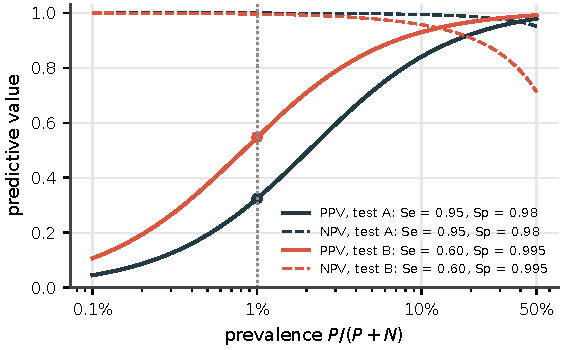
\includegraphics[width=0.72\textwidth]{ch01/prevalence_ppv}
\caption{Positive (solid) and negative (dashed) predictive values as a function of prevalence
for two tests. The dots mark the PPV at a prevalence of 1\%.}
\label{fig:prevalence}
\end{figure}

\begin{example}{What is the sensitivity of a COVID-19 test?}{covid}
During the COVID-19 pandemic, rapid antigen tests were criticised because, compared with PCR,
they missed a substantial fraction of infections. \citet{mina2020rethinking} argued that this
comparison used the wrong reference for the purpose of \emph{containment}. PCR detects viral
RNA long before and long after a person is infectious, whereas antigen tests detect the high
viral loads typical of the infectious period. If the goal is to stop transmission, what
matters is the sensitivity for \emph{infectious} people, and also how often and how fast
results are obtained: a cheap test used frequently, with immediate results, can prevent more
transmission than a very sensitive test whose result arrives two days later.

The lesson goes beyond medicine: a metric is only meaningful with respect to a reference
(what counts as a ``true'' positive) and to the context in which the model is deployed.
\end{example}

\subsection{Multiclass problems}

With $c$ classes the confusion matrix\index{confusion matrix} $M$ is $c\times c$, with $M_{jk}$ the number of examples
predicted as class $j$ whose actual class is $k$. Per-class metrics are obtained by treating
each class as positive and the rest as negative (\emph{one-versus-all\index{one-versus-all|textbf}}, OVA): for class $j$,
$\TP_j=M_{jj}$, $\FP_j=\sum_{k\neq j}M_{jk}$ (rest of the row) and $\FN_j=\sum_{k\neq j}M_{kj}$
(rest of the column). The per-class results are then averaged:
\begin{itemize}
  \item \emph{macro} average: plain mean over classes, which gives the same weight to every
        class and therefore emphasises small classes;
  \item \emph{weighted} average: mean weighted by the number of examples of each class, which
        reflects the class distribution of the test set;
  \item \emph{micro} average: the counts $\TP_j$, $\FP_j$, $\FN_j$ are pooled before
        computing the metric. In single-label problems micro precision, micro recall and
        micro $F_1$ all equal the accuracy.
\end{itemize}
Metrics defined only for two classes can also be extended with the \emph{one-versus-one\index{one-versus-one|textbf}}
(OVO) approach, which computes $c(c-1)/2$ results, one for each pair of classes.

\begin{example}{Three classes}{multiclass}
A classifier of animal pictures produces the following confusion matrix on 20 test images
(rows: predicted; columns: actual):
\begin{center}\small
\begin{tabular}{@{}lccc@{}}
\toprule
{\footnotesize pred.\,\textbackslash\,actual} & cat & dog & rabbit\\
\midrule
cat    & 8 & 1 & 0\\
dog    & 2 & 4 & 1\\
rabbit & 0 & 1 & 3\\
\bottomrule
\end{tabular}
\end{center}
For \emph{dog}: $\TP=4$, $\FP=2+1=3$ and $\FN=1+1=2$, so precision is $4/7=0.571$ and recall
$4/6=0.667$. \Cref{lst:multiclass} computes all the per-class and averaged values (note that
the matrix is written transposed in the code, following scikit-learn's convention). The
accuracy is 0.75; the macro-averaged\index{macro-average} $F_1$ (0.736) is lower than the weighted one (0.756)
because the worst class, \emph{dog}, counts as much as \emph{cat} in the macro average.
\end{example}

\begin{pylisting}[label={lst:multiclass}]{Per-class and averaged metrics for the three-class example}
import numpy as np
from sklearn.metrics import classification_report

cm = np.array([[8, 2, 0],      # rows: actual class (cat, dog, rabbit)
               [1, 4, 1],      # columns: predicted class
               [0, 1, 3]])
y_true = np.repeat(np.arange(3), cm.sum(axis=1))
y_pred = np.concatenate([np.repeat(np.arange(3), row) for row in cm])
print(classification_report(y_true, y_pred, digits=3,
                            target_names=["cat", "dog", "rabbit"]))
\end{pylisting}
\begin{pyoutput}
              precision    recall  f1-score   support

         cat      0.889     0.800     0.842        10
         dog      0.571     0.667     0.615         6
      rabbit      0.750     0.750     0.750         4

    accuracy                          0.750        20
   macro avg      0.737     0.739     0.736        20
weighted avg      0.766     0.750     0.756        20
\end{pyoutput}

% ---------------------------------------------------------------------
\section{ROC analysis}\label{sec:roc}

\subsection{Origins: signal detection}

Receiver Operating Characteristic\index{ROC analysis} (ROC) analysis originated in signal detection theory,
developed to analyse radar signals during the Second World War and later used extensively in
psychophysics and medical diagnosis \citep{green1966signal}. The problem is to decide whether
a signal is present in a noisy observation. If the observations follow one distribution when
there is only noise and another when signal is present, any decision rule\index{decision rules} of the form ``say
\emph{signal} if the observation exceeds a threshold $t$'' trades hits (true positives)
against false alarms (false positives), and the best threshold depends on the strength of the
signal, on the noise variance and on the hit or false alarm rate we are willing to accept
(\cref{fig:signal}). \citet{spackman1989signal} was one of the first to use ROC graphs to
evaluate machine learning algorithms.

\begin{figure}[htbp]
\centering
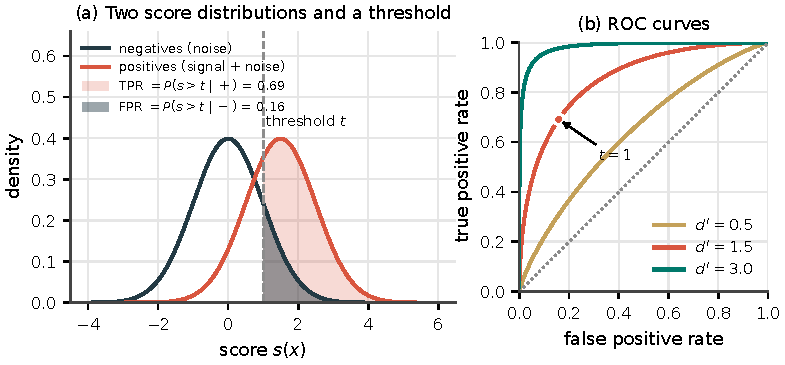
\includegraphics[width=\textwidth]{ch01/signal_detection}
\caption{(a) Scores of negatives $\mathcal N(0,1)$ and positives $\mathcal N(1.5,1)$; a threshold
$t=1$ gives $\TPR=0.69$ and $\FPR=0.16$. (b) Moving the threshold traces a ROC curve; the
curve depends on the separation $d'$ between the two distributions.}
\label{fig:signal}
\end{figure}

\subsection{The ROC space}

A crisp classifier is represented in the \emph{ROC space\index{ROC space|textbf}} by the point $(\FPR,\TPR)$. For
instance, a classifier with $\TP=3$, $\FN=1$, $\FP=3$ and $\TN=7$ has $\TPR=3/4=0.75$ and
$\FPR=3/10=0.30$, point A in \cref{fig:rocspace}. Some points are special:
\begin{itemize}
  \item $(0,0)$ is the classifier that always predicts negative (AlwaysNeg) and $(1,1)$ the one
        that always predicts positive (AlwaysPos);
  \item $(0,1)$ is the perfect classifier (``ROC heaven'') and $(1,0)$ the classifier that is
        always wrong (``ROC hell'');
  \item a classifier that predicts positive at random with probability $p$ lies at $(p,p)$:
        the diagonal contains all the random classifiers;
  \item a classifier below the diagonal is worse than random, but it contains useful
        information: inverting its predictions maps $(\FPR,\TPR)$ to $(1-\FPR,1-\TPR)$, a point
        above the diagonal (A$'$ becomes A in \cref{fig:rocspace}).
\end{itemize}
Since both coordinates are computed within one actual class, the position of a classifier in
ROC space does not depend on the class distribution or on the costs. This is what makes ROC
analysis\index{ROC analysis} useful when the deployment context is uncertain.

\begin{figure}[htbp]
\centering
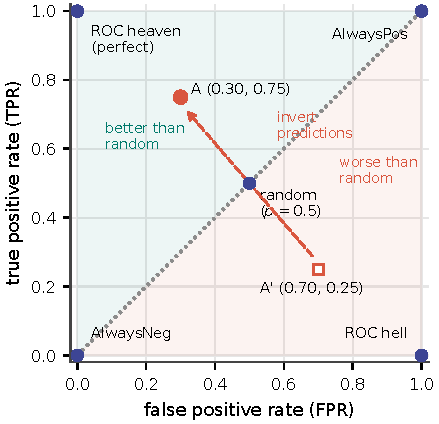
\includegraphics[width=0.58\textwidth]{ch01/roc_space}
\caption{The ROC space. Points above the diagonal are better than random; a classifier below
it can be improved by inverting its predictions.}
\label{fig:rocspace}
\end{figure}

\subsection{Iso-performance lines and the ROC convex hull}

Assume that correct predictions cost nothing and that a false negative and a false positive
cost $c_{\mathrm{FN}}$ and $c_{\mathrm{FP}}$. The expected cost\index{expected cost} per example of a classifier
at $(\FPR,\TPR)$ is
\begin{equation}\label{eq:rocost}
  \text{Cost}=\pi_+\,(1-\TPR)\,c_{\mathrm{FN}}+\pi_-\,\FPR\,c_{\mathrm{FP}}.
\end{equation}
All the classifiers with the same expected cost lie on a straight line
$\TPR=m\cdot\FPR+b$, an \emph{iso-performance line}, with slope
\begin{equation}\label{eq:isoslope}
  m=\frac{\pi_-\,c_{\mathrm{FP}}}{\pi_+\,c_{\mathrm{FN}}}=\frac{N}{P}\cdot\frac{c_{\mathrm{FP}}}{c_{\mathrm{FN}}}.
\end{equation}
For accuracy (equal costs) the slope is simply the class ratio $C=N/P$, and the lines are
called \emph{iso-accuracy\index{iso-accuracy line|textbf}\index{accuracy|textbf} lines} \citep{flach2003geometry}. Steep lines (many negatives or
expensive false positives) favour conservative classifiers close to $(0,0)$; flat lines
favour liberal classifiers close to $(1,1)$.

To find the best classifier for a given slope, move a line with that slope from the
upper-left corner towards the lower right until it touches a classifier. The classifiers that
can be touched first lie on the \emph{ROC convex hull\index{ROC convex hull|textbf}} (ROCCH) of the set of points, including
the trivial classifiers $(0,0)$ and $(1,1)$ \citep{provost2001robust}. Hence:
\begin{itemize}
  \item classifiers below the hull are never optimal, whatever the class distribution or the
        costs;
  \item each vertex of the hull is optimal for the range of slopes between the slopes of its
        two adjacent segments;
  \item any point on a segment of the hull can be achieved by choosing randomly, for each
        example, between the two classifiers at its ends.
\end{itemize}

\begin{example}{Choosing a classifier for each context}{rochull}
Five classifiers have been evaluated on the same test set:
\begin{center}\small
\begin{tabular}{@{}lccccc@{}}
\toprule
& CN2 & Ripper & C4.5 & NB & SVM\\
\midrule
FPR\index{false positive rate} & 0.05 & 0.10 & 0.16 & 0.28 & 0.60\\
TPR\index{true positive rate} & 0.50 & 0.60 & 0.80 & 0.70 & 0.95\\
\bottomrule
\end{tabular}
\end{center}
The convex hull is $(0,0)\to\text{CN2}\to\text{C4.5}\to\text{SVM}\to(1,1)$, with segment slopes
$10$, $2.73$, $0.34$ and $0.125$; Ripper and NB lie below it (\cref{fig:rochull}).
\begin{itemize}
  \item With balanced classes, $C=1$ lies between 2.73 and 0.34, so C4.5 is optimal, with
        accuracy $0.5\cdot0.80+0.5\cdot(1-0.16)=0.82$.
  \item With four times more positives than negatives, $C=1/4$ lies between 0.34 and 0.125:
        SVM is optimal, with accuracy $0.8\cdot0.95+0.2\cdot0.40=0.84$.
  \item With four times more negatives, $C=4$ lies between 10 and 2.73: CN2 is optimal, with
        accuracy $0.2\cdot0.50+0.8\cdot0.95=0.86$.
  \item AlwaysNeg is optimal when $C>10$, that is, when less than $1/11\approx9\%$ of the
        examples are positive; AlwaysPos is optimal when $C<0.125$, that is, when less than
        $1/9\approx11\%$ are negative.
\end{itemize}
No classifier is the best in all contexts, and two of them are the best in none.
\end{example}

\begin{figure}[htbp]
\centering
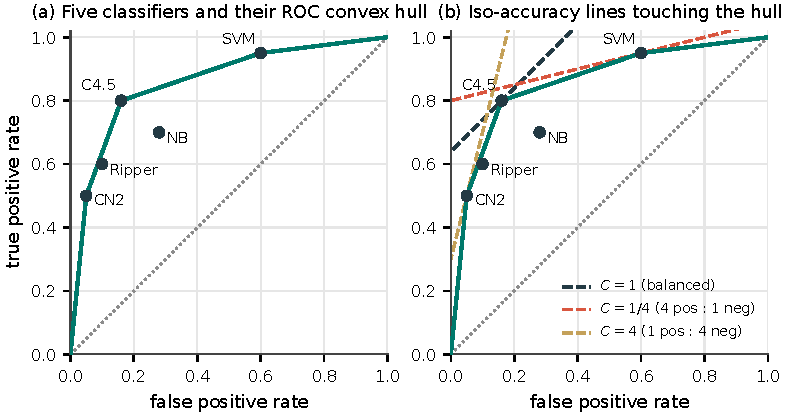
\includegraphics[width=\textwidth]{ch01/roc_hull}
\caption{(a) The ROC convex hull of the five classifiers of \cref{ex:rochull}. (b) The
iso-accuracy lines for three class ratios touch the hull at the optimal classifier for each
context.}
\label{fig:rochull}
\end{figure}

\subsection{Scoring classifiers and ROC curves}

Most classifiers can output a \emph{score} rather than a label: a scoring classifier\index{scoring classifier} assigns
to each example a real-valued score $s(x)$, with larger values indicating stronger evidence for the positive class,
such as a predicted positive-class probability or a signed decision margin. Ratios are useful in specific cases, such
as posterior odds or a likelihood ratio $P(x\mid+)/P(x\mid-)$ with a positive denominator; arbitrary class scores need
not admit such an interpretation (with scores $g(x)$ and $-g(x)$ for the two classes, the ratio is always $-1$). Any
strictly increasing transformation of $s(x)$ ranks the examples in the same order; a merely non-decreasing one can
create ties. A scoring classifier is therefore a \emph{ranker}, and it becomes a
crisp classifier by fixing a threshold $t$: predict positive if $s(x)\geq t$. Each threshold
gives a point in ROC space\index{ROC space}, and moving the threshold from $+\infty$ to $-\infty$ traces the
\emph{ROC curve\index{ROC curve|textbf}} of the ranker. \Cref{alg:roc} builds it from a test set
\citep{fawcett2006introduction}.

\begin{algorithm}[htbp]
\caption{Construction of a ROC curve}\label{alg:roc}
\begin{algorithmic}[1]
\Require test examples with scores $s(x_i)$ and actual classes; numbers of positives $P$ and negatives $N$
\State sort the examples by decreasing score
\State $(\mathit{fpr},\mathit{tpr})\gets(0,0)$ and output this point
\For{each group of examples with the same score, in decreasing order of score}
  \State $p\gets$ number of positives in the group; $q\gets$ number of negatives in the group
  \State $(\mathit{fpr},\mathit{tpr})\gets(\mathit{fpr}+q/N,\ \mathit{tpr}+p/P)$
         \Comment{diagonal step if the group mixes classes}
  \State output $(\mathit{fpr},\mathit{tpr})$
\EndFor
\end{algorithmic}
\end{algorithm}

In words: start at $(0,0)$ and walk down the ranking; each positive moves the curve up by
$1/P$, each negative moves it right by $1/N$, and a group of tied scores containing both
classes produces a diagonal step.

\begin{example}{Building a ROC curve}{roccurve}
Ten test examples receive the following scores (sorted in decreasing order):
\begin{center}\small
\setlength{\tabcolsep}{4.5pt}
\begin{tabular}{@{}lcccccccccc@{}}
\toprule
Score & 0.95 & 0.90 & 0.85 & 0.80 & 0.70 & 0.70 & 0.60 & 0.55 & 0.40 & 0.20\\
Class & $+$ & $+$ & $-$ & $+$ & $+$ & $-$ & $-$ & $+$ & $-$ & $-$\\
\bottomrule
\end{tabular}
\end{center}
With $P=N=5$, the curve goes up twice (to $(0,0.4)$), right once (0.85, a negative), up once
(0.80), then diagonally from $(0.2,0.6)$ to $(0.4,0.8)$ because of the tie at 0.70, right
(0.60), up (0.55) and right twice (\cref{fig:roccurve}). Its area is 0.78 (\cref{lst:roc}).
\end{example}

\begin{figure}[htbp]
\centering
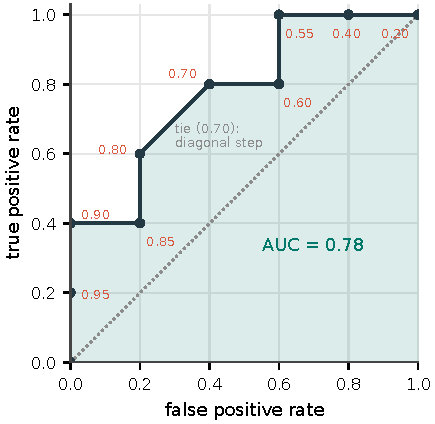
\includegraphics[width=0.56\textwidth]{ch01/roc_construction}
\caption{ROC curve of the ranking of \cref{ex:roccurve}. Each point is labelled with the
threshold that produces it; the shaded area is the AUC.}
\label{fig:roccurve}
\end{figure}

\subsection{The area under the ROC curve}

The \emph{area under the ROC curve\index{area under the ROC curve (AUC)|textbf}\index{ROC curve|textbf}} (AUC) summarises the whole curve in a single number
\citep{bradley1997use}. It has a very intuitive interpretation
\citep{hanley1982meaning}: the AUC is the probability that a randomly chosen positive
receives a higher score than a randomly chosen negative, which is the Mann--Whitney\index{Mann--Whitney--Wilcoxon statistic}--Wilcoxon
statistic \citep{mann1947test}:
\begin{equation}\label{eq:auc}
  \mathrm{AUC}=\frac{1}{P\cdot N}\sum_{i:\,y_i=+}\ \sum_{k:\,y_k=-} I\bigl(s(x_i),s(x_k)\bigr),
  \qquad
  I(a,b)=\begin{cases}1 & a>b,\\ 0.5 & a=b,\\ 0 & a<b.\end{cases}
\end{equation}
In the multiclass notation of \cref{sec:scoring}, the AUC of class $j$ against class $k$
using the probabilities estimated for class $j$ is
\begin{equation}
  \mathrm{AUC}(j,k)=\frac{\sum_{i=1}^{n}f(i,j)\sum_{t=1}^{n}f(t,k)\,I\bigl(p(i,j),p(t,j)\bigr)}{n_j\cdot n_k},
\end{equation}
where $n_j$ and $n_k$ are the numbers of examples of each class. In \cref{ex:roccurve}, 19.5 of
the 25 positive--negative pairs are correctly ordered (the tie counts one half), so
$\mathrm{AUC}=0.78$, as \cref{lst:roc} confirms.

\begin{pylisting}[label={lst:roc}]{ROC curve and AUC, computed by scikit-learn and by counting pairs}
import numpy as np
from sklearn.metrics import roc_curve, roc_auc_score

y = np.array([1, 1, 0, 1, 1, 0, 0, 1, 0, 0])                     # actual class
s = np.array([.95, .90, .85, .80, .70, .70, .60, .55, .40, .20])  # scores
fpr, tpr, thr = roc_curve(y, s)
print("FPR:", fpr.round(2))
print("TPR:", tpr.round(2))
print("AUC (scikit-learn):", roc_auc_score(y, s))

# AUC as the Mann-Whitney-Wilcoxon statistic: compare all (pos, neg) pairs
pos, neg = s[y == 1], s[y == 0]
diff = pos[:, None] - neg[None, :]
print("AUC (pairs):       ", ((diff > 0) + 0.5 * (diff == 0)).mean())
\end{pylisting}
\begin{pyoutput}
FPR: [0.  0.  0.  0.2 0.2 0.4 0.6 0.6 1. ]
TPR: [0.  0.2 0.4 0.4 0.6 0.8 0.8 1.  1. ]
AUC (scikit-learn): 0.78
AUC (pairs):        0.78
\end{pyoutput}

The AUC has several useful properties:
\begin{itemize}
  \item it is 1 for a perfect ranking, 0.5 for a random one, and below 0.5 for a ranking
        worse than random;
  \item it only depends on the order of the scores: any increasing transformation of the
        scores leaves it unchanged. It says nothing about whether the scores are good
        probabilities (\cref{sec:calibration});
  \item like the ROC curve, it does not depend on the class distribution;
  \item in credit scoring it is often reported as the \emph{Gini coefficient},
        $\mathrm{Gini}=2\,\mathrm{AUC}-1$;
  \item a crisp classifier has a ``curve'' with only three points, $(0,0)$, $(\FPR,\TPR)$
        and $(1,1)$, and its area is $(1+\TPR-\FPR)/2$, which is exactly its balanced
        accuracy\index{balanced accuracy} (Exercise~\ref{exr:aucba}).
\end{itemize}

\Cref{fig:rocmodels} compares four classifiers on the same synthetic problem. The random forest
dominates the other three almost everywhere (AUC 0.902), whereas the curves of logistic
regression (0.823) and naive Bayes\index{naive Bayes} (0.828) cross: which of the two is preferable depends on the
region of the curve where the model will operate. ROC curves are therefore very useful to
select the best model for a particular context of deployment, and the AUC is the right summary
when that context is unknown. When the relevant region is known (for instance, a screening
programme that cannot tolerate more than 10\% of false alarms) the \emph{partial} AUC over that
region is more informative.

\begin{figure}[htbp]
\centering
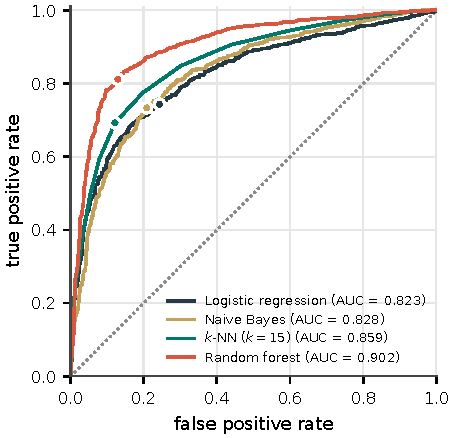
\includegraphics[width=0.6\textwidth]{ch01/roc_models}
\caption{ROC curves of four classifiers on a synthetic problem (2000 test examples). The dots
show the crisp classifiers obtained with the default threshold 0.5.}
\label{fig:rocmodels}
\end{figure}

\begin{further}
\citet{hand2009measuring} pointed out that the AUC implicitly averages over misclassification
costs using a distribution that depends on the classifier itself, and proposed the
H-measure as an alternative. \citet{hernandez2012unified} gave a unifying view: accuracy, AUC,
the Brier score\index{Brier score} and other metrics are all \emph{expected losses}, under different assumptions
about how the decision threshold will be chosen when the model is deployed. Choosing a metric
is, implicitly, choosing such an assumption.
\end{further}

\subsection{Multiclass ROC analysis}

A full ROC analysis\index{ROC analysis} with $c$ classes would need a space of $c(c-1)$ dimensions. In practice
the AUC is extended by averaging binary AUCs:
\begin{itemize}
  \item \emph{one-versus-rest}: one AUC per class against all the others, averaged either
        uniformly or weighted by the prior class distribution;
  \item \emph{one-versus-one\index{one-versus-one|textbf}}: the measure $M$ of \citet{hand2001simple} averages over all
        pairs of classes,
        \begin{equation*}
          M=\frac{2}{c(c-1)}\sum_{j<k}\hat A(j,k),\qquad
          \hat A(j,k)=\frac{\mathrm{AUC}(j,k)+\mathrm{AUC}(k,j)}{2},
        \end{equation*}
        and it is insensitive to the class distribution.
\end{itemize}
In scikit-learn, these variants are selected with the arguments \code{multi_class}
(\code{"ovr"} or \code{"ovo"}) and \code{average} (\code{"macro"} or \code{"weighted"}) of
\code{roc_auc_score}.

\subsection{Cumulative gains and lift charts}

In marketing and customer relationship management\index{customer relationship management (CRM)} (Unit~7) a model is used to rank customers,
and only the top-ranked fraction is contacted. The \emph{cumulative gains\index{cumulative gains chart|textbf} chart} plots the
fraction of all the positives (for instance, responders to a campaign\index{mailing campaign}) found among the top
$q$ fraction of the ranking, and the \emph{lift\index{lift|textbf}} is the ratio between that fraction and $q$,
i.e.\ how many times better than random targeting the model is. In the example of
\cref{fig:gains}, with 5\% of responders, contacting the top 20\% of customers reaches 76\% of
the responders, a lift of 3.78. The gains chart is closely related to the ROC curve\index{ROC curve}: its
horizontal axis is the fraction of examples predicted positive,
$\pi_+\TPR+\pi_-\FPR$, which is close to the $\FPR$ when positives are rare.

\begin{figure}[htbp]
\centering
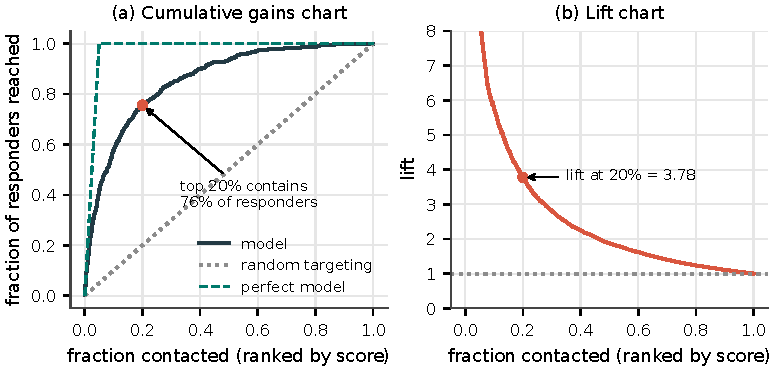
\includegraphics[width=\textwidth]{ch01/gains_lift}
\caption{Cumulative gains (a) and lift (b) of a ranking model for a mailing campaign with a 5\%
response rate (10,000 customers).}
\label{fig:gains}
\end{figure}

% ---------------------------------------------------------------------
\section{Evaluating probabilistic predictions}\label{sec:scoring}

Many applications need more than a label or a ranking: they need \emph{probabilities}. A bank
computing the expected loss of a loan, a doctor explaining a risk to a patient, or a system
combining the outputs of several models all rely on the probabilities being meaningful.

\subsection{Notation}

Consider a test set with $n$ examples and $c$ classes. Let $p(i,j)\in[0,1]$ be the probability
estimated by the model that example $i$ belongs to class $j$ (with $\sum_j p(i,j)=1$), and let
$f(i,j)\in\{0,1\}$ be the observed one-hot class indicator, which is 1 if example $i$ belongs to class $j$
and 0 otherwise. The true conditional probabilities $P(Y=j\mid x_i)$ are generally unknown: the measures
below compare the predicted probabilities with the observed outcomes. In binary problems we write $\hat p_i=p(i,+)$ and $y_i=f(i,+)$.

\subsection{Absolute error, Brier score and logarithmic loss}

The \emph{mean absolute error\index{mean absolute error (MAE)|textbf}} measures how much the predicted probabilities deviate from the
observed one-hot outcomes,
\begin{equation}
  \mathrm{MAE}=\frac{1}{n\,c}\sum_{j=1}^{c}\sum_{i=1}^{n}\bigl|f(i,j)-p(i,j)\bigr|.
\end{equation}
The \emph{mean squared error\index{mean squared error (MSE)|textbf}} is its quadratic version, which penalises strong deviations
much more:
\begin{equation}
  \mathrm{MSE}=\frac{1}{n\,c}\sum_{j=1}^{c}\sum_{i=1}^{n}\bigl(f(i,j)-p(i,j)\bigr)^2.
\end{equation}
For binary problems the two terms of the inner sum are equal and the MSE reduces to the
\emph{Brier score\index{Brier score|textbf}} \citep{brier1950verification},
$\mathrm{BS}=\frac1n\sum_i(y_i-\hat p_i)^2$.\footnote{Brier's original multiclass definition
sums over the classes without dividing by $c$, so it ranges from 0 to 2. Always check which
normalisation a library uses.}
Finally, the \emph{logarithmic loss\index{log loss|textbf}} (or cross-entropy) measures the probability assigned to
the actual class:
\begin{equation}
  \mathrm{LogLoss}=-\frac1n\sum_{i=1}^{n}\sum_{j=1}^{c}f(i,j)\log p(i,j)
                 =-\frac1n\sum_{i=1}^{n}\log p(i,y_i).
\end{equation}
It takes values in $[0,\infty)$, it is 0 only for perfect and fully confident predictions, and
it penalises confident mistakes without limit: assigning probability close to zero to the
actual class costs almost infinitely. Implementations clip the probabilities to
$[\epsilon,1-\epsilon]$ to avoid infinite values. The logarithm can be natural (as in
scikit-learn) or in base~2 (the loss is then measured in bits).

\begin{example}{Which metrics notice a better probability?}{scoringex}
A model assigns the following probabilities of being positive to five test examples:
\begin{center}\small
\begin{tabular}{@{}lccccc@{}}
\toprule
$\hat p(+)$ & 0.80 & 0.70 & 0.60 & 0.55 & 0.40\\
Actual class & $+$ & $-$ & $+$ & $+$ & $-$\\
\bottomrule
\end{tabular}
\end{center}
\begin{itemize}
  \item \emph{ROC curve\index{ROC curve|textbf} and AUC\index{area under the ROC curve (AUC)|textbf}.} With $P=3$ and $N=2$ the curve goes
        $(0,0)\to(0,\tfrac13)\to(\tfrac12,\tfrac13)\to(\tfrac12,\tfrac23)\to(\tfrac12,1)\to(1,1)$,
        and its area is $\tfrac12\cdot\tfrac13+\tfrac12\cdot1=\tfrac23$. Counting pairs gives the
        same result: of the $3\times2=6$ positive--negative pairs, four are correctly ordered.
  \item \emph{Accuracy\index{accuracy|textbf}} with threshold 0.5: only the second example is misclassified, 0.80.
  \item \emph{Brier score}:
        $(0.2^2+0.7^2+0.4^2+0.45^2+0.4^2)/5=1.0525/5=0.2105$.
\end{itemize}
If the probability of the third example increases from 0.60 to 0.68, the ranking does not
change (0.68 is still below 0.70) and neither does any prediction, so AUC and accuracy are
unchanged; but the Brier score (0.1990) and the log loss improve, because the model is now
more confident about a correct prediction (\cref{lst:scoring}).
\end{example}

\begin{pylisting}[label={lst:scoring}]{Effect of improving one probability on four metrics}
import numpy as np
from sklearn.metrics import roc_auc_score, accuracy_score, brier_score_loss, log_loss

y = np.array([1, 0, 1, 1, 0])
for p3 in (0.60, 0.68):                       # probability given to the third example
    p = np.array([0.80, 0.70, p3, 0.55, 0.40])
    print(f"p3={p3:.2f}  AUC={roc_auc_score(y, p):.3f}  "
          f"Acc={accuracy_score(y, p >= 0.5):.2f}  "
          f"Brier={brier_score_loss(y, p):.4f}  LogLoss={log_loss(y, p):.4f}")
\end{pylisting}
\begin{pyoutput}
p3=0.60  AUC=0.667  Acc=0.80  Brier=0.2105  LogLoss=0.6093
p3=0.68  AUC=0.667  Acc=0.80  Brier=0.1990  LogLoss=0.5843
\end{pyoutput}

\subsection{Proper scoring rules}

Which of these metrics actually rewards good probabilities? A \emph{scoring rule} $S(p,y)$
assigns a loss to the prediction $p$ when the outcome is $y$. It is \emph{proper} if, whenever
the true probability of the event is $q$, the expected loss $\E_{Y\sim q}[S(p,Y)]$ is minimised
by predicting $p=q$, and \emph{strictly proper} if $q$ is the only minimiser
\citep{gneiting2007strictly}. In other words, a proper scoring rule\index{proper scoring rule} never rewards a model for
reporting something different from what it believes. For a binary event:
\begin{itemize}
  \item Brier score\index{Brier score}: $\E[S]=q(1-p)^2+(1-q)p^2$, whose derivative $2(p-q)$ vanishes at $p=q$:
        strictly proper;
  \item log loss\index{log loss}: $\E[S]=-q\log p-(1-q)\log(1-p)$, whose derivative $-q/p+(1-q)/(1-p)$ vanishes
        at $p=q$: strictly proper;
  \item absolute error: $\E[S]=q(1-p)+(1-q)p=q+p(1-2q)$, which is \emph{linear} in $p$ and is
        minimised by $p=1$ if $q>1/2$ and by $p=0$ if $q<1/2$: \emph{not} proper.
\end{itemize}

\begin{keyidea}
The MAE\index{mean absolute error (MAE)} of probabilities rewards overconfidence: a model that rounds its probabilities to 0
or 1 obtains a better expected MAE than an honest one. Use the Brier score or the log loss to
judge probabilities. Both are strictly proper and, as we will see, they reward both
calibration and discrimination.
\end{keyidea}

\subsection{A taxonomy of classification metrics}

\citet{ferri2009experimental} compared 18 classification metrics experimentally over many data
sets and models, and found three families whose members are strongly correlated with each
other but much less with members of other families (\cref{tab:taxonomy}). The family to use
depends on how the model will be used.

\begin{table}[htbp]
\centering\small
\caption{Three families of classification metrics \citep{ferri2009experimental}.}\label{tab:taxonomy}
\begin{tabularx}{\textwidth}{@{}>{\raggedright\arraybackslash}p{3.2cm}>{\raggedright\arraybackslash}p{3.6cm}X@{}}
\toprule
Family & Examples & Use when\dots\\
\midrule
Threshold and qualitative understanding of error & accuracy, macro-averaged accuracy,
$F$-measure, kappa & the model makes decisions with a fixed threshold and we want to
minimise the number (or cost) of errors.\\
Probabilistic understanding of error & MAE, MSE (Brier score), log loss & we need an
assessment of the reliability of the probabilities (risk estimation, combination of models,
decisions with changing costs).\\
Ranking quality & AUC & the model prioritises cases: mailing campaigns, customer relationship
management, recommender systems, fraud detection.\\
\bottomrule
\end{tabularx}
\end{table}

\begin{example}{Metrics can disagree}{disagree}
Consider two binary classifiers $M_1$ and $M_2$ and a test set $T$. Each of the following
situations can happen, as \cref{lst:disagree} verifies:
\begin{enumerate}[label=(\alph*)]
  \item \emph{MAE\index{mean absolute error (MAE)|textbf} prefers $M_1$, MSE\index{mean squared error (MSE)|textbf} prefers $M_2$.} Two positive examples. $M_1$ predicts
        $(1.0, 0.2)$: one perfect and one bad prediction (MAE 0.40, MSE 0.32). $M_2$ predicts
        $(0.55,0.55)$: two mediocre predictions (MAE 0.45, MSE 0.20). The squared error
        punishes the single large error of $M_1$.
  \item \emph{Accuracy\index{accuracy|textbf} prefers $M_1$, MAE prefers $M_2$.} Actual classes $(+,+,-,-)$. $M_1$
        predicts $(0.51,0.51,0.49,0.49)$: all correct at threshold 0.5, but barely (accuracy
        1, MAE 0.49). $M_2$ predicts $(0.99,0.99,0.01,0.60)$: confident and almost always
        right (accuracy 0.75, MAE 0.16).
  \item \emph{Accuracy prefers $M_1$, AUC\index{area under the ROC curve (AUC)|textbf} prefers $M_2$.} Same actual classes. $M_1$ predicts
        $(0.90,0.40,0.30,0.45)$: accuracy 0.75, AUC 0.75. $M_2$ predicts $(0.90,0.80,0.70,0.60)$:
        a perfect ranking (AUC 1) with a bad threshold, since everything is predicted
        positive (accuracy 0.5).
\end{enumerate}
\end{example}

\begin{pylisting}[label={lst:disagree}]{Three pairs of models on which two metrics disagree}
import numpy as np
from sklearn.metrics import roc_auc_score

mae = lambda y, p: np.mean(np.abs(y - p))
mse = lambda y, p: np.mean((y - p) ** 2)
acc = lambda y, p: np.mean((p >= 0.5) == y)

y = np.array([1, 1])                                   # (a) MAE vs. MSE
m1, m2 = np.array([1.0, 0.2]), np.array([0.55, 0.55])
print(f"(a) MAE: {mae(y, m1):.3f} vs {mae(y, m2):.3f} | "
      f"MSE: {mse(y, m1):.3f} vs {mse(y, m2):.3f}")
y = np.array([1, 1, 0, 0])                             # (b) accuracy vs. MAE
m1, m2 = np.array([.51, .51, .49, .49]), np.array([.99, .99, .01, .60])
print(f"(b) Acc: {acc(y, m1):.2f} vs {acc(y, m2):.2f} | "
      f"MAE: {mae(y, m1):.3f} vs {mae(y, m2):.3f}")
m1, m2 = np.array([.90, .40, .30, .45]), np.array([.90, .80, .70, .60])
print(f"(c) Acc: {acc(y, m1):.2f} vs {acc(y, m2):.2f} | "    # (c) accuracy vs. AUC
      f"AUC: {roc_auc_score(y, m1):.2f} vs {roc_auc_score(y, m2):.2f}")
\end{pylisting}
\begin{pyoutput}
(a) MAE: 0.400 vs 0.450 | MSE: 0.320 vs 0.202
(b) Acc: 1.00 vs 0.75 | MAE: 0.490 vs 0.158
(c) Acc: 0.75 vs 0.50 | AUC: 0.75 vs 1.00
\end{pyoutput}

% ---------------------------------------------------------------------
\section{Calibration}\label{sec:calibration}

\subsection{What is a calibrated model?}

A binary probabilistic classifier is \emph{well calibrated\index{calibration|textbf}} if, among the examples that receive
a predicted probability $p$, the proportion of positives is approximately $p$:
\begin{equation}
  P\bigl(Y=1\mid\hat p(X)=p\bigr)=p\qquad\text{for all }p.
\end{equation}
A calibrated weather forecaster is one for whom it rains on about 70\% of the days with a 70\%
forecast. Calibration is different from discrimination (ranking quality). A model that always
predicts the prevalence\index{prevalence} is perfectly calibrated but without discrimination (it can still be a useful
reference); a model that ranks perfectly can
be badly calibrated, since any increasing transformation of its scores keeps its AUC. Good
probabilistic models need both properties, and proper scoring rules\index{proper scoring rule} reward both: the Brier
score\index{Brier score} decomposes into a calibration term and a refinement term
\citep{degroot1983comparison}.

Not all learning methods produce calibrated probabilities. Naive Bayes is a clear example: its
independence assumption counts correlated evidence several times and pushes the probabilities
towards 0 and 1. Maximum-margin methods such as SVMs output distances to a hyperplane, not
probabilities; boosted trees tend to avoid extreme values; and modern deep networks are often
overconfident \citep{niculescu2005predicting,guo2017calibration}. As we will see in
\cref{sec:imbalance}, resampling and class weights also distort the probabilities.

\subsection{Reliability diagrams}

A \emph{reliability diagram\index{calibration!reliability diagram|textbf}} (or calibration plot) groups the test examples into bins of
predicted probability and plots, for each bin, the mean predicted probability against the
observed fraction of positives. A calibrated model follows the diagonal. A histogram of the
predicted probabilities, shown alongside, tells how many examples support each point.

\Cref{fig:reliability} compares four models trained on the same data. Logistic regression,
which directly optimises the log loss\index{log loss}, is close to the diagonal. Naive Bayes concentrates its
probabilities near 0 and 1 and is \emph{overconfident}: when it predicts 0.9, the observed
frequency is much lower. The SVM, whose decision values have been naively rescaled to $[0,1]$,
is \emph{underconfident}: its outputs cluster around 0.5 while the actual frequencies are much
more extreme, which produces the typical sigmoid-shaped curve. In this example the random
forest is reasonably calibrated.

\begin{figure}[htbp]
\centering
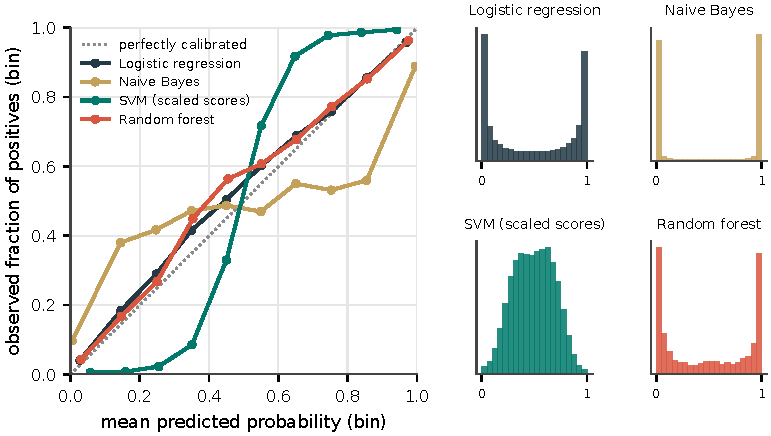
\includegraphics[width=\textwidth]{ch01/reliability}
\caption{Reliability diagrams (left) and histograms of predicted probabilities (right) of four
models trained on 1000 examples and tested on 99,000.}
\label{fig:reliability}
\end{figure}

\subsection{Measuring calibration}

Most calibration measures segment the test examples into bins and estimate the local
calibration error in each bin:
\begin{itemize}
  \item the \emph{expected calibration\index{calibration|textbf} error\index{calibration!expected calibration error|textbf}} \citep{naeini2015obtaining} averages the
        calibration gaps of $B$ bins, weighted by their sizes:
        \begin{equation}
          \mathrm{ECE}=\sum_{b=1}^{B}\frac{|S_b|}{n}\,\bigl|\bar y_b-\bar p_b\bigr|,
        \end{equation}
        where $\bar y_b$ and $\bar p_b$ are the fraction of positives and the mean predicted
        probability in bin $b$. The \emph{maximum calibration error} (MCE) takes the maximum
        gap instead. In the example of \cref{fig:reliability}, the ECE is 0.020 for logistic
        regression, 0.107 for naive Bayes\index{naive Bayes}, 0.203 for the rescaled SVM and 0.023 for the
        random forest. ECE depends on the number and type (equal width or equal frequency) of
        bins and is biased for small samples;
  \item \emph{CalBin\index{calibration!CalBin and CalLoss|textbf}} uses overlapping bins: the examples are sorted by predicted probability,
        a sliding window of consecutive examples (for instance 100) moves along the ranking,
        and the absolute differences between the mean probability and the fraction of
        positives in each window are averaged, as in the CAL measure of \citet{caruana2004data};
        other versions average the deviation of each individual prediction from the fraction of
        positives of its window \citep{ferri2009experimental}, so the variant used must be stated;
  \item \emph{CalLoss} derives the bins from the segments of the ROC convex hull\index{ROC convex hull}, which
        coincide with the blocks produced by isotonic regression\index{calibration!isotonic regression}
        \citep{fawcett2007pav}. The slope $m$ of a segment is a likelihood ratio, not a probability: with
        a proportion $\pi$ of positives, the empirical probability of the positive class in the
        segment is $m\pi/(m\pi+1-\pi)$ (for instance $2/3$ for $m=2$ and balanced classes). The
        calibration loss is the mean squared deviation between the predicted probabilities and
        these empirical probabilities; \citet{ferri2009experimental} group equal predicted
        probabilities instead of hull segments, so here too the variant must be stated. A measure
        computed on evaluation data is a diagnostic; a calibrator to deploy must be fitted on
        separate calibration data;
  \item the MSE\index{mean squared error (MSE)} and the log loss\index{log loss} also measure calibration, mixed with discrimination. For
        forecasts that take $K$ distinct values $p_k$ ($n_k$ examples each, with a fraction
        $\bar y_k$ of positives, and an overall fraction $\bar y$), the Brier score\index{Brier score} decomposes
        exactly \citep{murphy1973new} as
        \begin{equation}\label{eq:murphy}
          \mathrm{BS}=\underbrace{\frac1n\sum_k n_k(p_k-\bar y_k)^2}_{\text{reliability}}
                     -\underbrace{\frac1n\sum_k n_k(\bar y_k-\bar y)^2}_{\text{resolution}}
                     +\underbrace{\bar y(1-\bar y)}_{\text{uncertainty}}.
        \end{equation}
        Reliability measures calibration (lower is better), resolution measures how well the
        forecasts separate cases with different outcome frequencies (higher is better), and
        uncertainty depends only on the data. Grouping the uncertainty and the resolution
        gives the decomposition of the Brier score into \emph{calibration} and
        \emph{refinement} \citep{degroot1983comparison}. With continuous forecasts, binning
        makes the decomposition approximate.
\end{itemize}

\begin{pitfall}
\textbf{Small samples flatter hulls and calibration errors.} On small or very imbalanced\index{class imbalance} validation sets, the
convex hull of noisy ROC points, the isotonic fit behind CalLoss and the bins of the ECE all adapt to the noise:
the area under the hull is optimistic, and the calibration errors are biased (the ECE is positive even for a
perfectly calibrated model). Estimate them on data that took no part in fitting the hull or the calibrator, and
report their variability, for instance with the bootstrap\index{bootstrap}.
\end{pitfall}

\subsection{Calibration methods}

\emph{Calibrating} a classifier consists of fitting a regressor (the \emph{calibrator}) that
maps the scores of the classifier to calibrated probabilities. The examples used to train the
calibrator must not have been used to train the classifier, because scores on training data
are optimistic; scikit-learn's \code{CalibratedClassifierCV} handles this with an internal
cross-validation. The most common calibrators are:
\begin{itemize}
  \item \emph{Platt scaling\index{calibration!Platt scaling|textbf}} \citep{platt1999probabilistic}: a logistic regression on the
        score $s$, $\hat p=1/\bigl(1+\exp(As+B)\bigr)$, with $A$ and $B$ fitted by maximum
        likelihood. It has only two parameters, needs little data and corrects
        sigmoid-shaped distortions such as those of SVMs;
  \item \emph{isotonic regression\index{calibration!isotonic regression|textbf}} \citep{zadrozny2002transforming}: fits a non-parametric,
        non-decreasing step function with the pool-adjacent-violators (PAV) algorithm. It can
        correct any monotone distortion but needs more data, since it can overfit small
        calibration sets. It is equivalent to calibrating with the ROC convex hull\index{ROC convex hull}
        \citep{fawcett2007pav};
  \item \emph{temperature scaling} \citep{guo2017calibration}: for multiclass neural networks,
        divides the logits $z$ by a single parameter $T>0$ fitted on validation data,
        $\hat p=\operatorname{softmax}(z/T)$. It does not change the predicted class, so the
        accuracy is unchanged. It mainly improves \emph{confidence} (top-label) calibration,
        $P(Y=\hat y\mid\max_j\hat p_j=p)=p$; \emph{classwise} calibration, $P(Y=j\mid\hat p_j=p)=p$ for every
        class $j$, is a stronger requirement that a single parameter cannot always meet, which motivates
        vector, matrix and Dirichlet calibration \citep{kull2019beyond};
  \item \emph{beta calibration\index{calibration|textbf}} \citep{kull2017beta}: a three-parameter family that contains
        the identity map, designed for scores that are already in $[0,1]$.
\end{itemize}

\Cref{fig:calibmethods} calibrates an SVM like that of \cref{fig:reliability}, trained on a different sample: Platt scaling reduces
the ECE\index{calibration!expected calibration error} from 0.285 to 0.032 and isotonic regression to 0.007. \Cref{lst:calibration} does the
same for naive Bayes\index{naive Bayes} and reports the three probabilistic metrics: the log loss\index{log loss} falls from 1.15
to 0.28, mostly because the overconfident mistakes disappear. A strictly increasing
calibrator applied to a fixed score preserves the ranking and the AUC. Isotonic regression can
introduce ties, and when, as in the listing, the calibrated probabilities of models fitted on
different folds are averaged, the ranking can also change; here the AUC hardly moves. Calibration matters most when the probabilities are used
to take decisions, as in \cref{sec:costs}.

\begin{figure}[htbp]
\centering
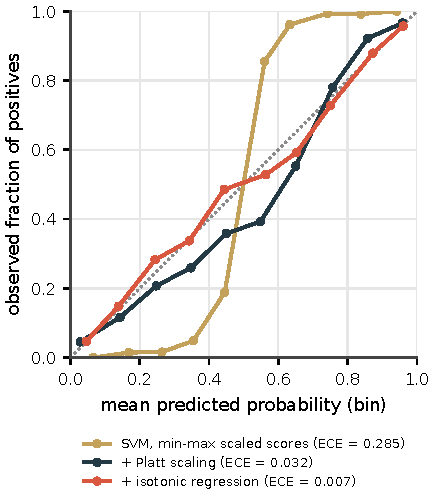
\includegraphics[width=0.56\textwidth]{ch01/calibration_methods}
\caption{Reliability diagrams of a linear SVM with naively rescaled scores, and of the same
model calibrated with Platt scaling and isotonic regression (20,000 test examples).}
\label{fig:calibmethods}
\end{figure}

\begin{pylisting}[label={lst:calibration}]{Calibrating naive Bayes with Platt scaling and isotonic regression}
import numpy as np
from sklearn.calibration import CalibratedClassifierCV
from sklearn.datasets import make_classification
from sklearn.metrics import brier_score_loss, log_loss
from sklearn.model_selection import train_test_split
from sklearn.naive_bayes import GaussianNB

def ece(y, p, n_bins=10):
    """Expected calibration error with equal-width bins."""
    b = np.minimum((p * n_bins).astype(int), n_bins - 1)
    return sum(np.mean(b == k) * abs(y[b == k].mean() - p[b == k].mean())
               for k in range(n_bins) if np.any(b == k))

X, y = make_classification(n_samples=40000, n_features=20, n_informative=2,
                           n_redundant=10, random_state=42)
X_tr, X_te, y_tr, y_te = train_test_split(X, y, test_size=0.5, random_state=0)
models = {"NB": GaussianNB(),
          "NB + Platt": CalibratedClassifierCV(GaussianNB(), method="sigmoid", cv=5),
          "NB + isotonic": CalibratedClassifierCV(GaussianNB(), method="isotonic", cv=5)}
for name, m in models.items():
    p = m.fit(X_tr, y_tr).predict_proba(X_te)[:, 1]
    print(f"{name:14s} Brier={brier_score_loss(y_te, p):.4f}  "
          f"LogLoss={log_loss(y_te, p):.4f}  ECE={ece(y_te, p):.4f}")
\end{pylisting}
\begin{pyoutput}
NB             Brier=0.1050  LogLoss=1.1476  ECE=0.1009
NB + Platt     Brier=0.0960  LogLoss=0.3342  ECE=0.0171
NB + isotonic  Brier=0.0849  LogLoss=0.2809  ECE=0.0068
\end{pyoutput}

% ---------------------------------------------------------------------
\section{Imbalanced classification}\label{sec:imbalance}

In many important problems one class is rare: fraud, diseases, machine failures, customers
who respond to a campaign\index{mailing campaign}. Imbalance\index{class imbalance} affects both evaluation and learning.

\subsection{Why accuracy fails}

\begin{example}{Detecting a rare event}{valves}
A plant monitors 100,000 safety valves, of which 500 (0.5\%) are faulty (\emph{open}) and must
be inspected; the rest are \emph{closed}. Three classifiers produce these confusion matrices\index{confusion matrix}
(rows: predicted; columns: actual):
\begin{center}\small
\begin{tabular}{@{}lcc@{\qquad}lcc@{\qquad}lcc@{}}
\toprule
$c_1$ & open & close & $c_2$ & open & close & $c_3$ & open & close\\
\midrule
OPEN  & 300 & 500    & OPEN  & 0   & 0      & OPEN  & 400 & 5400\\
CLOSE & 200 & 99,000 & CLOSE & 500 & 99,500 & CLOSE & 100 & 94,100\\
\bottomrule
\end{tabular}
\end{center}
Their metrics are:
\begin{center}\small
\begin{tabular}{@{}lccc@{}}
\toprule
& $c_1$ & $c_2$ & $c_3$\\
\midrule
Error & 0.70\% & \textbf{0.50\%} & 5.50\%\\
TPR\index{true positive rate} / TNR & 60.0\% / 99.5\% & 0.0\% / 100\% & 80.0\% / 94.6\%\\
PPV\index{predictive value!positive} / NPV\index{predictive value!negative} & 37.5\% / 99.8\% & undefined / 99.5\% & 6.9\% / 99.9\%\\
Balanced accuracy\index{balanced accuracy} & 79.8\% & 50.0\% & \textbf{87.3\%}\\
G-mean & 0.773 & 0 & \textbf{0.870}\\
$F_1$ & \textbf{0.462} & 0 & 0.127\\
MCC\index{Matthews correlation coefficient} & \textbf{0.471} & 0 & 0.225\\
Kappa & \textbf{0.458} & 0 & 0.119\\
\bottomrule
\end{tabular}
\end{center}
The classifier with the lowest error, $c_2$, never detects a faulty valve: it simply predicts
the majority class. Balanced accuracy and the G-mean prefer $c_3$, which finds 80\% of the
faulty valves at the price of 5400 unnecessary inspections. $F_1$, MCC and kappa prefer $c_1$,
which is much more precise. Which one is better? The metrics cannot tell; only the
consequences of each type of error can. We will come back to this example in
\cref{sec:costs}.
\end{example}

\begin{keyidea}
When classes are imbalanced\index{class imbalance}, avoid metrics centred only on counting mistakes (accuracy,
error): the trivial majority classifier is hard to beat on them. Recommended alternatives are
the AUC and the average precision\index{average precision} for rankings, and the $F_1$ score, balanced accuracy,
G-mean and MCC for crisp decisions, ideally complemented by an explicit cost analysis.
\end{keyidea}

\subsection{Precision--recall analysis}

The \emph{precision\index{precision|textbf}--recall\index{recall|textbf}} (PR) curve plots precision against recall for all thresholds, and
the \emph{average precision\index{average precision|textbf}} (AP) summarises it as a step-wise area,
$\mathrm{AP}=\sum_k(R_k-R_{k-1})P_k$, where $P_k$ and $R_k$ are the precision and recall at the
$k$-th threshold. Unlike the ROC curve\index{ROC curve}, the PR curve depends on the class distribution: the
precision of a random classifier equals the prevalence\index{prevalence}. This is exactly why it is informative
with rare positives \citep{saito2015precision}. In \cref{fig:prvsroc} the same score
distributions are evaluated with 50\% and 2\% of positives. The ROC curves are almost
identical (AUC 0.857 and 0.862), but the average precision drops from 0.855 to 0.213: with
many negatives, even a small false positive rate\index{false positive rate} produces many false alarms, and most positive
predictions are wrong. The ROC curve hides this; the PR curve shows it.

\begin{figure}[htbp]
\centering
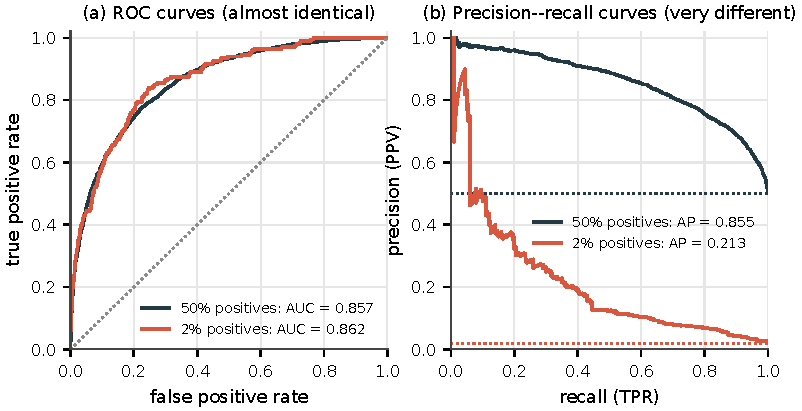
\includegraphics[width=\textwidth]{ch01/pr_vs_roc}
\caption{The same scoring model evaluated with 50\% and with 2\% of positives. (a) ROC curves
do not depend on the class distribution. (b) Precision--recall curves do; the dotted lines are
the precision of a random classifier (the prevalence).}
\label{fig:prvsroc}
\end{figure}

\citet{davis2006relationship} proved that a curve dominates another in ROC space\index{ROC space} if and only
if it dominates it in PR space, but that linear interpolation between points, valid in ROC
space, is not valid in PR space. This is why AP is computed as a step-wise sum rather than
with the trapezoidal rule.

\subsection{Learning from imbalanced data}

Many learning methods minimise the number of mistakes, and the learned models may simply
ignore the minority class \citep{japkowicz2002class,he2009learning}. The main remedies are:
\begin{itemize}
  \item \emph{undersampling\index{undersampling|textbf}} the majority class, which is fast but removes useful
        information;
  \item \emph{oversampling\index{oversampling|textbf}} the minority class by replication, which creates redundant
        examples and encourages overfitting;
  \item \emph{learning with costs or weights}, which minimises the (weighted) cost instead of
        the number of errors; in scikit-learn, \code{class_weight="balanced"} weights each
        class inversely to its frequency;
  \item \emph{synthetic oversampling}, which creates new minority examples.
\end{itemize}

The best known synthetic method is SMOTE\index{SMOTE}, the Synthetic Minority Oversampling Technique
\citep{chawla2002smote}. To create each synthetic example, SMOTE chooses a random minority
example, finds its $k$ (usually 5) nearest neighbours\index{k-nearest neighbours@$k$-nearest neighbours} of the same class, picks one of them at
random and creates a new example at a random point of the segment that joins the two
(\cref{fig:smote}). The core of the algorithm takes a few lines (\cref{lst:smote}).
Variants concentrate the new examples where they are most useful: Borderline-SMOTE near the
class boundary \citep{han2005borderline} and ADASYN where the minority class is harder to learn
\citep{he2008adasyn}. ROSE \citep{menardi2014training} uses a \emph{smoothed bootstrap\index{bootstrap|textbf}}
instead: it draws an example (choosing each class with equal probability) and generates a new
one from a kernel density centred on it, that is, from its neighbourhood.

\begin{figure}[htbp]
\centering
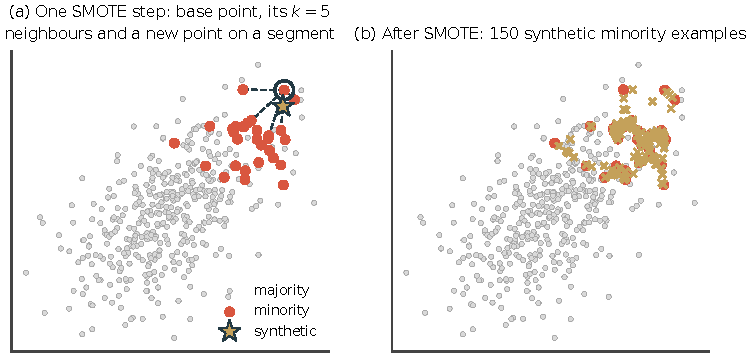
\includegraphics[width=\textwidth]{ch01/smote}
\caption{SMOTE. (a) A minority example (circled), its five nearest minority neighbours and a
synthetic example generated on one of the segments. (b) The data after adding 150 synthetic
examples.}
\label{fig:smote}
\end{figure}

\begin{pylisting}[label={lst:smote}]{A minimal implementation of SMOTE}
import numpy as np
from sklearn.neighbors import NearestNeighbors

def smote(X_min, n_new, k=5, seed=0):
    """Generate n_new synthetic minority examples (Chawla et al., 2002)."""
    rng = np.random.default_rng(seed)
    nn = NearestNeighbors(n_neighbors=k + 1).fit(X_min)
    _, idx = nn.kneighbors(X_min)                 # idx[:, 0] is the point itself
    base = rng.integers(0, len(X_min), n_new)      # random minority examples
    neigh = idx[base, rng.integers(1, k + 1, n_new)]   # one of their k neighbours
    gap = rng.random((n_new, 1))                   # random position on the segment
    return X_min[base] + gap * (X_min[neigh] - X_min[base])
\end{pylisting}

\begin{pitfall}
Resample only the training data. If SMOTE or any other resampling is applied before splitting
the data or before cross-validation, synthetic copies of test examples end up in the training
set and the evaluation is optimistic. The \code{Pipeline} of \textsf{imbalanced\index{class imbalance}-learn}
\citep{lemaitre2017imbalanced} applies the resampling only when fitting, inside each fold.
\end{pitfall}

\subsection{What rebalancing really does}

\Cref{lst:imbalance} compares, with 5-fold CV on a problem with about 3.5\% of positives (3\% before the label noise\index{label noise}
of the generator), a plain
logistic regression, a class-weighted one and SMOTE\index{SMOTE} followed by logistic regression. Rebalancing
increases the balanced accuracy\index{balanced accuracy} (from 0.60 to about 0.70) but \emph{decreases} the $F_1$ score
(from 0.33 to 0.15), slightly decreases the average precision\index{average precision}, and multiplies the Brier score\index{Brier score}
by seven.

\begin{pylisting}[label={lst:imbalance}]{Effect of class weights and SMOTE on four metrics}
from imblearn.over_sampling import SMOTE
from imblearn.pipeline import make_pipeline     # resamples ONLY the training folds
from sklearn.datasets import make_classification
from sklearn.linear_model import LogisticRegression
from sklearn.model_selection import StratifiedKFold, cross_validate

X, y = make_classification(n_samples=10000, n_features=10, n_informative=4,
                           weights=[0.97], flip_y=0.01, class_sep=1.5, random_state=0)
cv = StratifiedKFold(5, shuffle=True, random_state=0)
lr = lambda **kw: LogisticRegression(max_iter=1000, **kw)
models = {"plain LR": lr(),
          "weighted LR": lr(class_weight="balanced"),
          "SMOTE + LR": make_pipeline(SMOTE(random_state=0), lr())}
scoring = ["balanced_accuracy", "f1", "average_precision", "neg_brier_score"]
for name, m in models.items():
    r = cross_validate(m, X, y, cv=cv, scoring=scoring)
    print(f"{name:11s} BA={r['test_balanced_accuracy'].mean():.3f} "
          f"F1={r['test_f1'].mean():.3f} AP={r['test_average_precision'].mean():.3f} "
          f"Brier={-r['test_neg_brier_score'].mean():.4f}")
\end{pylisting}
\begin{pyoutput}
plain LR    BA=0.601 F1=0.331 AP=0.432 Brier=0.0250
weighted LR BA=0.697 F1=0.150 AP=0.377 Brier=0.1800
SMOTE + LR  BA=0.694 F1=0.148 AP=0.373 Brier=0.1771
\end{pyoutput}

In this experiment, rebalancing acts mostly like \emph{moving the decision threshold\index{threshold|textbf}}: the
rebalanced model predicts many more positives (more true positives and many more false
positives) without ranking the examples better. This is common but not guaranteed: changing the
weights or the sample also changes the fitted model, and with it the ranking, in ways that depend
on the learner and on the sampling method. And because the model has learned that positives are as
frequent as negatives, its probabilities no longer describe the original population. Under pure
prior shift\index{label shift}, when the class-conditional distributions do not change, the probabilities of a model
trained with a prevalence\index{prevalence} $\pi'$ can be corrected for a population with prevalence $\pi$ (random
sampling of whole classes approximates this situation; after SMOTE or other feature-dependent
sampling, recalibrate on data representative of deployment instead)
\citep{saerens2002adjusting,elkan2001foundations}:
\begin{equation}\label{eq:priorshift}
  \hat p=\frac{\frac{\pi}{\pi'}\,\hat p'}{\frac{\pi}{\pi'}\,\hat p'+\frac{1-\pi}{1-\pi'}\,(1-\hat p')}.
\end{equation}
For example, a model trained on balanced data ($\pi'=0.5$) that outputs $\hat p'=0.5$ for a
case from a population with $\pi=0.03$ corresponds to $\hat p=0.03$. In clinical risk
prediction, \citet{vandengoorbergh2022harm} showed that imbalance\index{class imbalance} corrections worsened the
calibration of logistic regression models without improving their discrimination.

\begin{keyidea}
Class imbalance is as much a problem of evaluation and decision as of learning. Often the
best strategy is to keep the data as they are, obtain calibrated probabilities, evaluate with
metrics suited to rare classes, and choose the threshold according to the costs
(\cref{sec:costs}).
\end{keyidea}

% ---------------------------------------------------------------------
\section{Cost-sensitive evaluation and learning}\label{sec:costs}

\subsection{Cost matrices}

Not all mistakes have the same consequences. In COVID-19 detection a false negative (an
infected person sent home) is much worse than a false positive (an unnecessary quarantine). In
credit granting, if the positive class is ``grant the loan'', a false positive (lending to
someone who will not pay back) usually costs much more than a false negative (losing the
margin of a good customer). A \emph{cost matrix\index{cost matrix|textbf}} $C$ states the cost of every possible
decision: $C(i,j)$ is the cost of predicting class $i$ when the actual class is $j$. It has the
same layout as the confusion matrix\index{confusion matrix} $M$, and the total cost of a classifier on a test set is
\begin{equation}
  \text{Cost}=\sum_{i=1}^{c}\sum_{j=1}^{c}C(i,j)\,M(i,j).
\end{equation}
Negative entries represent benefits.

\begin{example}{Total cost of a three-class model}{cost3}
A model classifies cases into three levels (\emph{low}, \emph{medium}, \emph{high}). The cost
matrix (left) and the confusion matrix on a test set (right), both with predicted classes in
rows and actual classes in columns, are:
\begin{center}\small
\begin{tabular}{@{}lrrr@{}}
\toprule
Cost & low & medium & high\\
\midrule
low    & 0\EUR    & 5\EUR      & 2\EUR\\
medium & 200\EUR  & $-2000$\EUR & 10\EUR\\
high   & 10\EUR   & 1\EUR      & $-15$\EUR\\
\bottomrule
\end{tabular}\qquad
\begin{tabular}{@{}lrrr@{}}
\toprule
Count & low & medium & high\\
\midrule
low    & 20 & 0  & 13\\
medium & 5  & 15 & 4\\
high   & 4  & 7  & 60\\
\bottomrule
\end{tabular}
\end{center}
Row by row, the costs are $0\cdot20+5\cdot0+2\cdot13=26$\EUR,
$200\cdot5-2000\cdot15+10\cdot4=-28{,}960$\EUR{} and $10\cdot4+1\cdot7-15\cdot60=-853$\EUR, so
the total cost is $-29{,}787$\EUR: the model produces a net benefit, almost entirely due to the
15 correctly identified \emph{medium} cases.
\end{example}

Returning to the valves of \cref{ex:valves}, suppose that an unnecessary inspection costs
100\EUR{} and an undetected faulty valve costs 2000\EUR. The total costs are
$500\cdot100+200\cdot2000=450{,}000$\EUR{} for $c_1$, $500\cdot2000=1{,}000{,}000$\EUR{} for
$c_2$ and $5400\cdot100+100\cdot2000=740{,}000$\EUR{} for $c_3$. Classifier $c_1$ is the best
choice, and $c_3$, preferred by balanced accuracy\index{balanced accuracy}, costs 64\% more.

\subsection{Optimal decisions from probabilities}

If a model provides calibrated probabilities $p(j\mid x)$, the expected cost\index{expected cost} of predicting
class $i$ for example $x$ is $\sum_j p(j\mid x)\,C(i,j)$, and the optimal decision is the class
with the lowest expected cost. With two classes and costs $c_{ij}$ (predicted $i$, actual $j$,
with 1 the positive class), predicting positive is optimal when
$p\,c_{11}+(1-p)\,c_{10}\leq p\,c_{01}+(1-p)\,c_{00}$, that is, when the probability of the
positive class exceeds the threshold
\begin{equation}\label{eq:tstar}
  t^\star=\frac{c_{10}-c_{00}}{(c_{10}-c_{00})+(c_{01}-c_{11})}
  \quad\text{or, if correct decisions cost nothing,}\quad
  t^\star=\frac{c_{\mathrm{FP}}}{c_{\mathrm{FP}}+c_{\mathrm{FN}}}
\end{equation}
\citep{elkan2001foundations}. For the valves, $t^\star=100/2100=0.048$: a valve should be
inspected whenever its probability of being open exceeds 4.8\%, far from the default 0.5.
\Cref{lst:costthreshold} applies this rule to a logistic regression on a problem with 3\% of
positives: moving the threshold from 0.5 to $t^\star$ multiplies the false positives by 200
but reduces the total cost by 32\%. \Cref{fig:costthreshold} shows the empirical cost as a
function of the threshold for three cost ratios; the minima are close to the theoretical
thresholds because logistic regression is well calibrated.

\begin{pylisting}[label={lst:costthreshold}]{Cost of the default threshold versus the Bayes-optimal one}
import numpy as np
from sklearn.datasets import make_classification
from sklearn.linear_model import LogisticRegression
from sklearn.model_selection import train_test_split

C_FP, C_FN = 100, 2000           # cost of a false alarm and of a missed positive
t_star = C_FP / (C_FP + C_FN)    # Bayes-optimal threshold for calibrated scores

X, y = make_classification(n_samples=40000, n_features=10, n_informative=5,
                           weights=[0.97], flip_y=0.01, random_state=3)
X_tr, X_te, y_tr, y_te = train_test_split(X, y, test_size=0.5, stratify=y,
                                          random_state=0)
p = LogisticRegression(max_iter=1000).fit(X_tr, y_tr).predict_proba(X_te)[:, 1]

def total_cost(y, yhat):
    return C_FP * np.sum((yhat == 1) & (y == 0)) + C_FN * np.sum((yhat == 0) & (y == 1))

for t in (0.5, t_star):
    yhat = (p >= t).astype(int)
    print(f"t={t:.4f}  FP={np.sum((yhat == 1) & (y_te == 0)):4d}  "
          f"FN={np.sum((yhat == 0) & (y_te == 1)):3d}  "
          f"cost={total_cost(y_te, yhat):>9,} EUR")
\end{pylisting}
\begin{pyoutput}
t=0.5000  FP=  14  FN=572  cost=1,145,400 EUR
t=0.0476  FP=3070  FN=235  cost=  777,000 EUR
\end{pyoutput}

\begin{figure}[htbp]
\centering
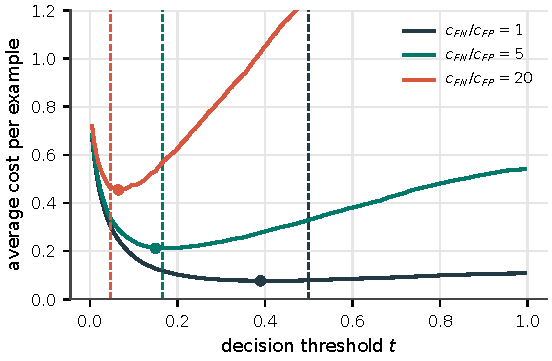
\includegraphics[width=0.7\textwidth]{ch01/cost_threshold}
\caption{Average cost per example (in units of $c_{\mathrm{FP}}$) as a function of the decision
threshold, for three cost ratios. Dashed lines: theoretical optimum $t^\star=1/(1+c_{\mathrm{FN}}/c_{\mathrm{FP}})$;
dots: empirical minimum.}
\label{fig:costthreshold}
\end{figure}

The same reasoning applies to more classes. With the cost matrix\index{cost matrix} of \cref{ex:cost3} and a case
with probabilities $(0.5, 0.3, 0.2)$ for \emph{low}, \emph{medium} and \emph{high}, the expected
costs are $0\cdot0.5+5\cdot0.3+2\cdot0.2=1.9$\EUR{} for predicting \emph{low},
$200\cdot0.5-2000\cdot0.3+10\cdot0.2=-498$\EUR{} for \emph{medium} and
$10\cdot0.5+1\cdot0.3-15\cdot0.2=2.3$\EUR{} for \emph{high}: the best decision is
\emph{medium}, although \emph{low} is the most probable class.

\subsection{Cost curves}

ROC space\index{ROC space} shows costs only indirectly, through the slopes of the iso-performance lines.
\emph{Cost curves\index{cost curve|textbf}} \citep{drummond2006cost} show them directly. The horizontal axis is the
\emph{probability cost}
\begin{equation}
  PC(+)=\frac{\pi_+\,c_{\mathrm{FN}}}{\pi_+\,c_{\mathrm{FN}}+\pi_-\,c_{\mathrm{FP}}}\in[0,1],
\end{equation}
which summarises the operating condition\index{operating point} (class distribution and costs) in a single number,
and the vertical axis is the \emph{normalised expected cost\index{expected cost|textbf}}
$\mathrm{NEC}=\FNR\cdot PC(+)+\FPR\cdot\bigl(1-PC(+)\bigr)$. Each classifier becomes a straight
line from $(0,\FPR)$ to $(1,\FNR)$; AlwaysNeg is the line $\mathrm{NEC}=PC(+)$ and AlwaysPos
the line $\mathrm{NEC}=1-PC(+)$. The lower envelope of all the lines gives the best achievable
cost for every operating condition, and it is the exact counterpart (the dual) of the ROC
convex hull\index{ROC convex hull}: points of ROC space become lines, and vertices of the hull become segments of the
envelope. \Cref{fig:costcurves} shows the five classifiers of \cref{ex:rochull}: we can read
directly the range of conditions in which each classifier is optimal and by how much it
improves on the others.

\begin{figure}[htbp]
\centering
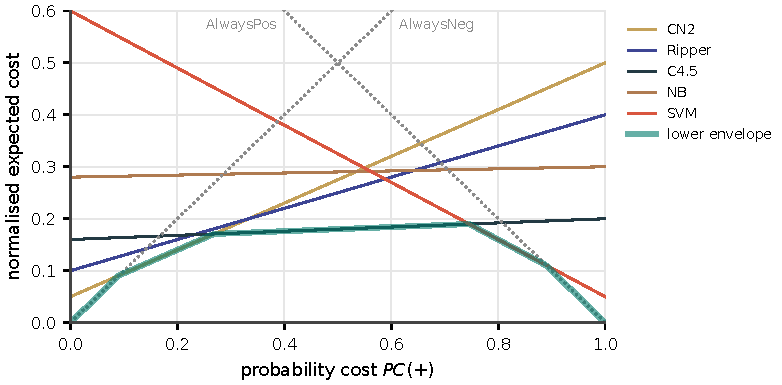
\includegraphics[width=0.75\textwidth]{ch01/cost_curves}
\caption{Cost curves of the five classifiers of \cref{ex:rochull}. The thick line is the lower
envelope, which corresponds to the ROC convex hull of \cref{fig:rochull}.}
\label{fig:costcurves}
\end{figure}

\subsection{Cost-sensitive learning strategies}

There are four main ways of making a learning process sensitive to costs:
\begin{enumerate}
  \item \emph{Expected cost\index{expected cost|textbf} minimisation (thresholding).} Train an ordinary probabilistic
        model, calibrate it if needed, and predict the class of minimum expected cost
        (\cref{eq:tstar}). It is simple, it works with any probabilistic model, and the
        costs can be changed after training.
  \item \emph{Resampling.} Change the class proportions of the training set so that a learner
        using the default threshold behaves as if it used $t^\star$. \citet{elkan2001foundations}
        showed that, if correct decisions cost nothing, the number of negative examples must be
        multiplied by $c_{\mathrm{FP}}/c_{\mathrm{FN}}$ (or, equivalently, positives replicated
        $c_{\mathrm{FN}}/c_{\mathrm{FP}}$ times). For the valves, one negative in every 20.
  \item \emph{Weighting.} Give each training example a weight proportional to the cost of
        misclassifying it \citep{zadrozny2003cost}. Most scikit-learn estimators accept
        \code{class_weight} or \code{sample_weight} for this purpose.
  \item \emph{Cost-sensitive\index{cost-sensitive learning|textbf} algorithms.} MetaCost\index{MetaCost} \citep{domingos1999metacost} estimates the
        class probabilities of the training examples with a bagged ensemble, relabels each
        training example with the class of minimum expected cost and retrains the base
        learner on the relabelled data, producing a single cost-sensitive model of the
        original type. AdaCost \citep{fan1999adacost} modifies boosting so that the weights of
        costly misclassified examples increase faster.
\end{enumerate}

\subsection{Other types of cost}

Misclassification costs are not the only costs. \citet{turney2000types} proposed a taxonomy of
nine types of cost in inductive learning, among which:
\begin{itemize}
  \item the cost of \emph{misclassification errors} (or prediction errors in general);
  \item the cost of \emph{tests}: obtaining the value of an attribute may require a laboratory
        analysis, a sensor or a questionnaire;
  \item the cost of the \emph{teacher}: labelling examples requires experts, which motivates
        active and semi-supervised\index{semi-supervised learning} learning;
  \item the cost of \emph{computation}: training and prediction time, memory and energy, which
        matter at deployment time (Unit~5);
  \item the cost of \emph{cases}: collecting data;
  \item the cost of \emph{instability}: models that change substantially when the data change
        slightly are hard to trust and to maintain, which is closely related to concept drift\index{concept drift}
        and to the need to update models (Unit~6).
\end{itemize}

\subsection{Test costs}

Knowing the exact value of some features has a cost. To diagnose a heart condition, the age of
the patient is free, the blood pressure is cheap and the cholesterol level requires a blood test.
When tests are costly, we want models that minimise the expected test cost\index{test costs} while keeping their
predictive performance. A model that needs every feature for every case, as most ensembles and
neural networks do, pays the full cost every time. A decision tree\index{decision tree} only asks for the tests on
the path followed by each case, and it can be induced to prefer cheap tests near the root
\citep{nunez1991use,turney1995cost}. For example, if a tree asks for the free attribute first,
for the blood pressure (5\EUR) in 60\% of the cases and for the cholesterol (40\EUR) in 20\%,
its expected test cost is $0.6\cdot5+0.2\cdot40=11$\EUR{} per patient, against 45\EUR{} for a
model that always requires all the tests. Evaluation should then report the expected
misclassification cost and the expected test cost together.

\subsection{Instance-dependent costs}

In some domains the cost of an error is not constant but varies from example to example.
\citet{elkan2001foundations} gives the example of credit card transactions, where $x$ is the
amount of the transaction. Here it is more convenient to use a \emph{benefit} matrix $B$ rather than a cost
matrix\index{cost matrix}: positive entries are gains and negative entries losses, and the optimal decision maximises the
expected benefit (equivalently, it minimises the costs $C=-B$):
\begin{center}\small
\begin{tabular}{@{}lcc@{}}
\toprule
{\footnotesize decision\,\textbackslash\,actual} & fraudulent & legitimate\\
\midrule
refuse  & $20$\EUR & $-20$\EUR\\
approve & $-x$     & $0.02\,x$\\
\bottomrule
\end{tabular}
\end{center}
Refusing a fraudulent transaction saves investigation and charge-back costs; refusing a
legitimate one annoys the customer; approving a fraudulent one loses the amount; approving a
legitimate one earns a 2\% commission. If $p$ is the probability of fraud, approving is better
than refusing when $0.02x(1-p)-xp>20p-20(1-p)$, that is, when
\begin{equation}
  p<\frac{0.02\,x+20}{1.02\,x+40}.
\end{equation}
The threshold is 0.40 for a 10\EUR{} transaction, 0.15 for 100\EUR{} and only 0.038 for
1000\EUR: large transactions are refused at much lower probabilities of fraud. During learning,
a simple approach is to re-weight each training example in proportion to its own
misclassification cost \citep{zadrozny2003cost}.

% ---------------------------------------------------------------------
\section{Evaluating regression models}\label{sec:regression}

In regression the model predicts a number, and the errors $e_i=\hat y_i-y_i$ have a magnitude
and a sign. Regression metrics differ in how they aggregate them.

\subsection{A worked example}

\Cref{tab:regex} shows the predictions of a model of the annual sales of ten companies (in
millions of euros). We will use it to illustrate all the metrics of this section.

\begin{table}[htbp]
\centering\small
\caption{Predicted and actual annual sales of ten companies (million \texteuro), with the
error $e=\hat y-y$ and its square.}\label{tab:regex}
\begin{tabular}{@{}lrrrrrrrrrr|r@{}}
\toprule
Company & 1 & 2 & 3 & 4 & 5 & 6 & 7 & 8 & 9 & 10 & Sum\\
\midrule
Predicted $\hat y$ & 100 & 102 & 105 & 95 & 101 & 105 & 105 & 40 & 220 & 100 &\\
Actual $y$         & 102 & 110 & 95  & 75 & 103 & 110 & 98  & 32 & 215 & 103 &\\
Error $e$          & $-2$ & $-8$ & 10 & 20 & $-2$ & $-5$ & 7 & 8 & 5 & $-3$ & 30\\
$|e|$              & 2 & 8 & 10 & 20 & 2 & 5 & 7 & 8 & 5 & 3 & 70\\
$e^2$              & 4 & 64 & 100 & 400 & 4 & 25 & 49 & 64 & 25 & 9 & 744\\
\bottomrule
\end{tabular}
\end{table}

\subsection{Error-based metrics}

Given a set $S$ of $n$ examples:
\begin{align}
  \mathrm{MAE}&=\frac1n\sum_{i=1}^n|y_i-\hat y_i|, &
  \mathrm{MSE}&=\frac1n\sum_{i=1}^n(y_i-\hat y_i)^2, &
  \mathrm{RMSE}&=\sqrt{\mathrm{MSE}}.
\end{align}
In the example, the \emph{mean absolute error\index{mean absolute error (MAE)|textbf}} is $70/10=7.0$, the \emph{mean squared error\index{mean squared error (MSE)|textbf}}
$744/10=74.4$ and the \emph{root mean squared error\index{root mean squared error (RMSE)|textbf}} 8.63 million euros. The RMSE is in the
units of the target and is always at least as large as the MAE; the gap between them grows
with the variability of the errors. The single error of 20 contributes 400 of the 744 squared
units: squared errors are dominated by the largest mistakes, which is desirable if large
errors are disproportionately harmful and undesirable if they come from outliers. Other
useful metrics are:
\begin{itemize}
  \item the \emph{median absolute error\index{median absolute error|textbf}}, robust to outliers: 6.0 in the example;
  \item the \emph{mean absolute percentage error\index{mean absolute percentage error|textbf}},
        $\mathrm{MAPE}=\frac1n\sum_i|y_i-\hat y_i|/|y_i|$: 9.0\% in the example. It is
        scale-free and easy to communicate, but it is undefined or explodes when $y_i$ is close
        to zero, and it is asymmetric: for a positive target an under-prediction can never cost
        more than 100\%, whereas an over-prediction is unbounded, so MAPE favours models that
        under-predict \citep{hyndman2006another};
  \item the \emph{mean absolute scaled error}, MASE, which divides the MAE by the in-sample
        MAE of a naive forecast (the previous value of the series). It is scale-free and a
        value below 1 means that the model beats the naive forecast \citep{hyndman2006another};
  \item the \emph{bias} or mean error, $\frac1n\sum_i(\hat y_i-y_i)$: $+3.0$ in the example.
        The model over-predicts by 3 million euros on average, something that neither MAE nor
        RMSE reveal.
\end{itemize}

\subsection{Relative metrics and the coefficient of determination}

Relative metrics compare the model with the trivial model that always predicts the mean
$\bar y$ of the target. The \emph{relative absolute error}
$\mathrm{RAE}=\sum_i|y_i-\hat y_i|/\sum_i|y_i-\bar y|$ is $70/244.2=0.287$ in the example. A
value below 1 means that the model is better than the mean, and a value above 1 that it is
worse: relative errors are not bounded by 1. The \emph{coefficient of determination\index{coefficient of determination@coefficient of determination ($R^2$)|textbf}}
\begin{equation}
  R^2=1-\frac{\sum_i(y_i-\hat y_i)^2}{\sum_i(y_i-\bar y)^2}
\end{equation}
is the proportion of the variance of the target explained by the model: $1-744/18{,}540.1=0.960$
in the example. On test data $R^2$ can be negative, when the model is worse than predicting the
mean. The \emph{explained variance score}, $1-\Var(y-\hat y)/\Var(y)=0.965$, ignores the
systematic bias of the predictions; it coincides with $R^2$ when the mean error is zero
(\cref{lst:regression}).

\begin{pitfall}
$R^2$ depends on the spread of the target in the test set. In the example it is very high
(0.96) mainly because the test set contains a very small and a very large company, which
inflate $\Var(y)$; yet errors of up to 20 million euros on companies selling around 100 million
may be unacceptable. Always report an absolute error measure as well.
\end{pitfall}

\begin{pylisting}[label={lst:regression}]{Regression metrics for the example of \cref{tab:regex}}
import numpy as np
from sklearn.metrics import (mean_absolute_error, mean_squared_error, r2_score,
                             median_absolute_error, mean_absolute_percentage_error,
                             explained_variance_score)

y_pred = np.array([100, 102, 105, 95, 101, 105, 105, 40, 220, 100])  # million EUR
y_true = np.array([102, 110, 95, 75, 103, 110, 98, 32, 215, 103])
rae = np.abs(y_true - y_pred).sum() / np.abs(y_true - y_true.mean()).sum()
print(f"MAE  = {mean_absolute_error(y_true, y_pred):.3f}")
print(f"MSE  = {mean_squared_error(y_true, y_pred):.3f}")
print(f"RMSE = {np.sqrt(mean_squared_error(y_true, y_pred)):.3f}")
print(f"MedAE= {median_absolute_error(y_true, y_pred):.3f}")
print(f"MAPE = {mean_absolute_percentage_error(y_true, y_pred):.4f}")
print(f"RAE  = {rae:.4f}")
print(f"R2   = {r2_score(y_true, y_pred):.4f}")
print(f"EV   = {explained_variance_score(y_true, y_pred):.4f}")
print(f"bias = {np.mean(y_pred - y_true):.3f}   (mean of yhat - y)")
\end{pylisting}
\begin{pyoutput}
MAE  = 7.000
MSE  = 74.400
RMSE = 8.626
MedAE= 6.000
MAPE = 0.0903
RAE  = 0.2867
R2   = 0.9599
EV   = 0.9647
bias = 3.000   (mean of yhat - y)
\end{pyoutput}

\subsection{Correlation-based metrics}

The \emph{Pearson\index{Pearson correlation|textbf} correlation} between predictions and actual values,
$r=\operatorname{cov}(y,\hat y)/(\sigma_y\sigma_{\hat y})$, measures their linear association,
and the \emph{Spearman\index{Spearman correlation|textbf} correlation}, the Pearson correlation between their ranks, measures any
monotone association. Both are invariant to (increasing linear or monotone) transformations of
the predictions: a model that predicts $\hat y=2y$ has a perfect correlation of 1, but its
errors are enormous (for $y=1,\dots,5$, $R^2=-4.5$). Correlations are useful to evaluate the
ability of a model to rank or to follow the trend of the target, not its accuracy.

\subsection{Residual analysis}

Single numbers hide structure. Plots of predicted against actual values and of residuals\index{residual analysis}
$y-\hat y$ against predictions (\cref{fig:residuals}) reveal curvature (a missing non-linear
effect), funnels (errors that grow with the prediction, which makes constant-width
prediction intervals inadequate; see \cref{sec:other}), outliers and groups of examples where
the model fails systematically. The diabetes data of \citet{efron2004least} used in the
figure show a typical situation: the residuals are centred on zero but widely spread
($R^2=0.35$), so much of the variability of the target remains unexplained.

\begin{figure}[htbp]
\centering
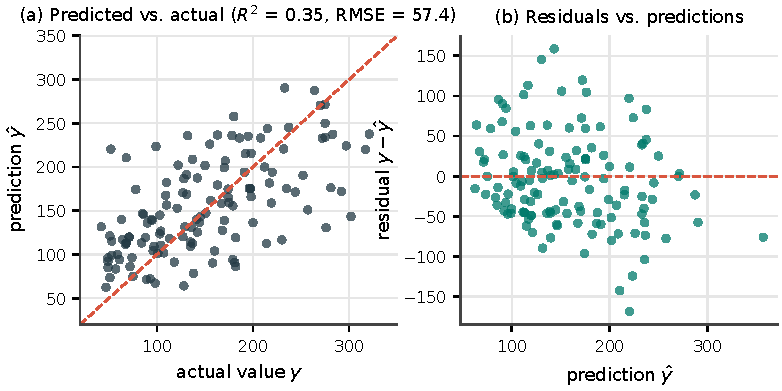
\includegraphics[width=\textwidth]{ch01/regression_diagnostics}
\caption{Diagnostic plots of a gradient boosting model on the diabetes data set (133 test
examples). (a) Predicted against actual values; (b) residuals against predictions.}
\label{fig:residuals}
\end{figure}

\subsection{Asymmetric costs}

Consider a supermarket that forecasts the demand of a product. An under-prediction causes a
\emph{stockout}: lost sales and unhappy customers. An over-prediction leaves surplus stock,
which costs storage or, for fresh products, is wasted. The two costs are rarely equal, so a
model ``centred'' on the expected demand is not the best option: the model that minimises the
MSE\index{mean squared error (MSE)} predicts the conditional mean, and the one that minimises the MAE\index{mean absolute error (MAE)} predicts the conditional
median, but neither takes the asymmetry into account. \Cref{fig:losses} compares several loss
functions.

\begin{figure}[htbp]
\centering
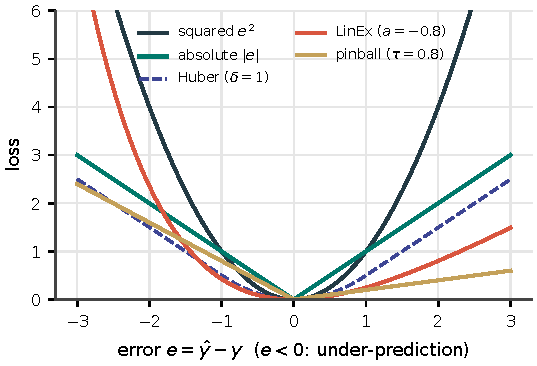
\includegraphics[width=0.72\textwidth]{ch01/regression_losses}
\caption{Loss functions as a function of the error $e=\hat y-y$. The LinEx loss with $a<0$ and
the pinball loss with $\tau>0.5$ penalise under-predictions more than over-predictions.}
\label{fig:losses}
\end{figure}

A popular asymmetric loss is the \emph{LinEx} loss \citep{zellner1986bayesian}, which is
approximately linear on one side and exponential on the other:
\begin{equation}
  L_a(e)=b\,\bigl(e^{a e}-a e-1\bigr),\qquad a\neq0,\ b>0.
\end{equation}
With $a>0$ over-predictions are penalised exponentially; with $a<0$, under-predictions. For
instance, with $a=-0.01$ and $b=1$, under-predicting the demand by 200 units costs
$L(-200)=e^{2}-3\approx4.39$, whereas over-predicting it by 200 units costs
$L(200)=e^{-2}+1\approx1.14$: being short is about four times worse than having a surplus. Note
that a function such as $1-e^{ae}$ is not a valid loss, since it is negative for errors of one
sign. With an asymmetric cost function we can select the model with the lowest average cost on
validation data or, better, train the model to minimise that cost directly.

Another important asymmetric loss is the \emph{pinball} (or quantile) loss, with
$\tau\in(0,1)$,
\begin{equation}\label{eq:pinball}
  L_\tau(y,\hat y)=\begin{cases}\tau\,(y-\hat y) & \text{if } y\geq\hat y,\\
                                 (1-\tau)\,(\hat y-y) & \text{if } y<\hat y,\end{cases}
\end{equation}
whose expected value is minimised by the $\tau$-quantile of the distribution of $y$ given $x$
\citep{koenker1978regression}. This gives a clean solution to the \emph{newsvendor problem}:
if each unit of unmet demand costs $c_u$ (underage) and each unsold unit costs $c_o$
(overage), the optimal prediction is the quantile
\begin{equation}
  \tau^\star=\frac{c_u}{c_u+c_o}.
\end{equation}
If a product has a margin of 3\EUR{} per unit sold and each unsold unit loses 1\EUR, the
forecast should target the 75th percentile of the demand, not its mean.

\begin{keyidea}
The optimal decision threshold of a classifier, $t^\star=c_{\mathrm{FP}}/(c_{\mathrm{FP}}+c_{\mathrm{FN}})$,
and the optimal quantile of a regressor, $\tau^\star=c_u/(c_u+c_o)$, have the same structure:
the costs of the two kinds of error determine the operating point\index{operating point}. A good model provides
calibrated probabilities or quantiles; the context decides how to use them.
\end{keyidea}

\subsection{Utility-based regression}

In many regression problems only some values of the target really matter: extreme rainfall,
very high returns of an investment, unusually high sales. \emph{Utility-based regression}
\citep{torgo2007utility} formalises this with a \emph{relevance function} $\phi(y)\in[0,1]$ that
marks the important values of the target, and a utility function that combines the benefits of
accurate predictions of relevant values with the costs of false alarms and missed events.
Models are then evaluated, selected and even trained to maximise utility rather than to
minimise a symmetric error. The cost penalties can also be added to standard regression
techniques so that they minimise the expected cost\index{expected cost} directly.

\subsection{Imbalanced regression}

When the values of interest are rare (extreme values of the target), regression suffers from
the same problem as imbalanced\index{class imbalance} classification: standard losses are dominated by the frequent
central values, and the model learns to ignore the extremes \citep{branco2016survey}. The
preprocessing strategies are analogous to those of classification: undersampling\index{undersampling} the common
values and oversampling\index{oversampling} the rare ones. \emph{SMOTE\index{SMOTE|textbf} for regression} (SMOTER) interpolates both
the inputs and the target between rare examples \citep{torgo2013smote}, and \emph{SMOGN}
combines random undersampling with two oversampling strategies, SMOTER and the addition of
Gaussian noise \citep{branco2017smogn}. Evaluation must then focus on the relevant values, for
example with errors restricted to them or with utility-based precision and recall, rather than
on a global MSE\index{mean squared error (MSE)}.

% ---------------------------------------------------------------------
\section{Other supervised settings}\label{sec:other}

\subsection{Ordinal regression}

In \emph{ordinal regression\index{ordinal regression|textbf}} (or ordinal classification) the classes have a natural order:
low $<$ medium $<$ high, star ratings, stages of a disease. Treating them as nominal classes
ignores that predicting \emph{high} for a \emph{low} case is worse than predicting
\emph{medium}; treating them as numbers assumes that consecutive classes are equally far
apart. Appropriate metrics \citep{gutierrez2016ordinal} include the MAE\index{mean absolute error (MAE)} computed on the ranks
of the classes, $\frac1n\sum_i|r(y_i)-r(\hat y_i)|$; rank correlations; and the
\emph{weighted kappa} \citep{cohen1968weighted},
\begin{equation}
  \kappa_w=1-\frac{\sum_{j,k}w_{jk}\,O_{jk}}{\sum_{j,k}w_{jk}\,E_{jk}},
  \qquad w_{jk}=\frac{(j-k)^2}{(c-1)^2},
\end{equation}
where $O_{jk}$ and $E_{jk}$ are the observed and the chance-expected proportions of examples
predicted as class $j$ with actual class $k$. The quadratic weights penalise distant errors
more than adjacent ones.

\subsection{Multi-label classification}

In \emph{multi-label\index{multi-label classification|textbf}} classification each example can have several non-exclusive labels
$Y_i\subseteq\mathcal L$: a news item can be about \emph{sports} and \emph{economy} at the same
time \citep{tsoumakas2007multi}. Suppose that the possible labels are \emph{sports},
\emph{politics} and \emph{economy}, that the actual labels of an example are
$\{$sports, economy$\}$ and that the predicted ones are $\{$sports, politics$\}$. Then:
\begin{itemize}
  \item the \emph{subset accuracy\index{accuracy|textbf}} (exact match) is 0, a very strict criterion;
  \item the \emph{Hamming loss}, the fraction of wrong label decisions,
        $\frac{1}{n|\mathcal L|}\sum_i|Y_i\,\triangle\,\hat Y_i|$, is $2/3$ (\emph{politics}
        wrongly added and \emph{economy} missed);
  \item the example-based \emph{Jaccard index} $|Y_i\cap\hat Y_i|/|Y_i\cup\hat Y_i|$ is $1/3$,
        and the example-based precision, recall and $F_1$ are all $1/2$;
  \item label-based metrics compute a binary metric for each label and average them with a
        micro or macro average\index{macro-average}, as in \cref{sec:crisp}.
\end{itemize}

\subsection{Hierarchical classification}

In \emph{hierarchical} classification the classes are organised in a tree or a directed acyclic
graph\index{causal graph} (animal $\to$ mammal $\to$ dog), and confusing two sibling classes is less serious than
confusing two distant ones. \emph{Hierarchical precision\index{precision|textbf} and recall\index{recall|textbf}} \citep{silla2011survey}
extend the sets of actual and predicted classes $C_i$ and $\hat C_i$ with all their ancestors
(except the root) and compute
\begin{equation}
  hP=\frac{\sum_i|\hat C_i\cap C_i|}{\sum_i|\hat C_i|},\qquad
  hR=\frac{\sum_i|\hat C_i\cap C_i|}{\sum_i|C_i|},\qquad
  hF=\frac{2\,hP\cdot hR}{hP+hR}.
\end{equation}
If a dog ($\{\text{animal},\text{mammal},\text{dog}\}$) is classified as a cat
($\{\text{animal},\text{mammal},\text{cat}\}$), $hP=hR=2/3$; if it is classified as a fish
($\{\text{animal},\text{fish}\}$), $hP=1/2$ and $hR=1/3$.

\subsection{Ranking and recommendation}

When the output of the model is an ordered list (search results, recommended products), what
matters is the quality of the first positions. Common metrics are \emph{precision\index{precision|textbf}@$k$} and
\emph{recall\index{recall|textbf}@$k$} (computed on the top $k$ items), the \emph{mean reciprocal rank\index{mean reciprocal rank|textbf}} (the average
of $1/\text{rank}$ of the first relevant item) and the \emph{normalised discounted cumulative
gain\index{NDCG|textbf}} \citep{jarvelin2002cumulated}:
\begin{equation}
  \mathrm{DCG@}k=\sum_{i=1}^{k}\frac{\mathit{rel}_i}{\log_2(i+1)},
  \qquad
  \mathrm{NDCG@}k=\frac{\mathrm{DCG@}k}{\mathrm{IDCG@}k},
\end{equation}
where $\mathit{rel}_i$ is the graded relevance of the item at position $i$ and IDCG is the DCG
of the ideal ordering. If the top three recommendations have relevances $(3,0,2)$,
$\mathrm{DCG@3}=3+0+2/2=4$; the ideal order $(3,2,0)$ gives $\mathrm{IDCG@3}=3+2/\log_2 3=4.26$,
and $\mathrm{NDCG@3}=0.94$. These metrics are studied in depth with recommender systems\index{recommender system}
(Unit~7).

\subsection{Conformal prediction}

A point prediction does not say how much we can trust it. \emph{Conformal prediction\index{conformal prediction|textbf}}
\citep{vovk2005algorithmic,angelopoulos2023conformal} is a framework for uncertainty
quantification\index{quantification} that turns any point predictor into one that outputs a \emph{set}: an interval
in regression, a set of labels in classification. These sets have a statistically valid
coverage\index{coverage} guarantee,
\begin{equation}
  P\bigl(Y_{n+1}\in\mathcal C(X_{n+1})\bigr)\geq1-\alpha,
\end{equation}
for any model and any data distribution, under the only assumption that the data are
exchangeable (for instance, independent and identically distributed). The simplest version,
\emph{split conformal\index{conformal prediction!split|textbf} prediction}, is shown in \cref{alg:conformal} and \cref{lst:conformal}.

\begin{algorithm}[htbp]
\caption{Split conformal prediction for regression}\label{alg:conformal}
\begin{algorithmic}[1]
\Require training set; calibration set $\{(x_i,y_i)\}_{i=1}^{n_{\text{cal}}}$; miscoverage level $\alpha$
\State fit a model $\hat h$ on the training set
\State compute the \emph{nonconformity scores} $s_i=|y_i-\hat h(x_i)|$ on the calibration set
\State $k\gets\lceil(n_{\text{cal}}+1)(1-\alpha)\rceil$; $\hat q\gets$ the $k$-th smallest score, or $\hat q\gets\infty$ if $k>n_{\text{cal}}$
\State \Return for each new $x$, the interval $\mathcal C(x)=\bigl[\hat h(x)-\hat q,\ \hat h(x)+\hat q\bigr]$
\end{algorithmic}
\end{algorithm}

If the required order is $n_{\text{cal}}+1$ (with 10 calibration scores and $\alpha=0.01$, for instance), the threshold is
infinite: the calibration sample cannot support a finite interval at the requested coverage without additional
assumptions.

\begin{pylisting}[label={lst:conformal}]{Split conformal prediction with a 90\% coverage target}
import numpy as np
from sklearn.ensemble import GradientBoostingRegressor

rng = np.random.default_rng(2)
X = rng.uniform(0, 10, (8000, 1))
y = X[:, 0] * np.sin(X[:, 0]) + rng.normal(0, 0.3 + 0.3 * X[:, 0])  # noisier for large x
idx = rng.permutation(len(y))
tr, cal, te = idx[:2000], idx[2000:4000], idx[4000:]   # train / calibration / test

alpha = 0.1                                           # target coverage 90%
model = GradientBoostingRegressor(random_state=0).fit(X[tr], y[tr])
scores = np.abs(y[cal] - model.predict(X[cal]))       # nonconformity scores
assert 0 < alpha < 1 and len(scores) > 0
k = int(np.ceil((len(cal) + 1) * (1 - alpha)))
q = np.inf if k > len(scores) else np.sort(scores)[k - 1]   # conformal quantile
pred = model.predict(X[te])
covered = (y[te] >= pred - q) & (y[te] <= pred + q)
print(f"q = {q:.3f};  interval width = {2 * q:.2f}")
print(f"empirical coverage = {covered.mean():.3f}  (target {1 - alpha:.2f})")
\end{pylisting}
\begin{pyoutput}
q = 3.516;  interval width = 7.03
empirical coverage = 0.903  (target 0.90)
\end{pyoutput}

The guarantee is \emph{marginal}: it holds on average over all the inputs (and over the
calibration sample, so a single run can fall slightly below $1-\alpha$). It does not hold for
every region of the input space. In \cref{fig:conformal}a the noise grows with $x$, but the
split conformal intervals have constant width: they cover 99.9\% of the test points with
$x<3$ and only 76.5\% of those with $x>7$, and the overall coverage is 90.3\%.
\emph{Conformalised quantile regression\index{conformal prediction!quantile regression|textbf}\index{quantile regression|textbf}} \citep{romano2019conformalized} starts from two quantile
regression models, trained with the pinball loss\index{pinball loss} of \cref{eq:pinball}, and conformalises their
interval; its intervals adapt to the noise (\cref{fig:conformal}b), with coverages of 93.5\%
and 91.1\% in the two regions and narrower intervals on average (6.18 against 7.03).

\begin{figure}[htbp]
\centering
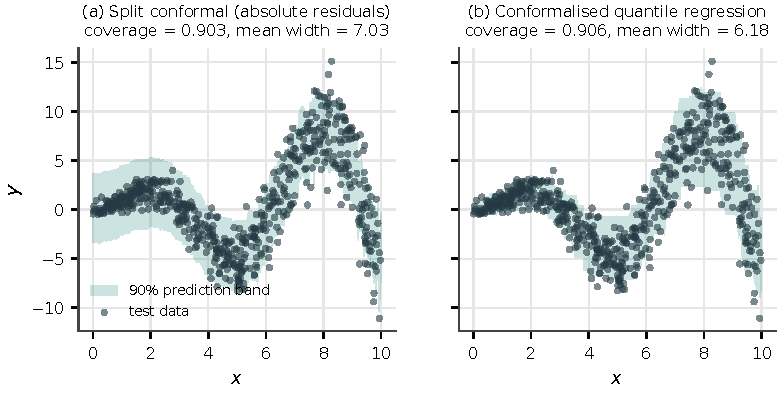
\includegraphics[width=\textwidth]{ch01/conformal}
\caption{90\% conformal prediction bands on data whose noise grows with $x$ (4000 test
points; 600 shown). (a) Split conformal with absolute residuals; (b) conformalised quantile
regression.}
\label{fig:conformal}
\end{figure}

In classification, the nonconformity score is usually $s_i=1-\hat p(y_i\mid x_i)$, and the
prediction set contains all the labels $y$ with $1-\hat p(y\mid x)\leq\hat q$: easy inputs get a
single label, ambiguous ones several. Conformal predictors are evaluated by their empirical
coverage (overall and in relevant subgroups) and by their \emph{efficiency}: at the same
coverage, narrower intervals or smaller sets are better.

\subsection{Semi-supervised learning}

In \emph{semi-supervised\index{semi-supervised learning|textbf} learning} a small amount of labelled data is combined with a large
amount of unlabelled data, which helps to discover the structure of the input space (for
instance, by placing the decision boundary in low-density regions) \citep{vanengelen2020survey}.
Evaluation must always use held-out \emph{labelled} data, and it is easy to get wrong.
\citet{oliver2018realistic} recommend comparing against well-tuned supervised baselines that
use the same model and tuning budget; using realistically small validation sets (tuning
hyperparameters with 5000 labelled validation examples makes no sense if only 250 labels are
supposed to be available); reporting performance as a function of the number of labels; and
checking what happens when the unlabelled data contain classes absent from the labelled data.

\subsection{Open-set recognition}

Standard classifiers assume a \emph{closed set}: the classes seen at test time are those seen
during training. In an \emph{open-set\index{open-set recognition|textbf}} scenario \citep{scheirer2013toward} the model may
encounter classes never seen during training: a model trained to recognise cars, dogs and
people will sooner or later receive a helicopter. A closed-set classifier is forced to assign
one of the known labels, often with high confidence (a \emph{high-confidence false
positive}). An open-set classifier must classify the known classes correctly \emph{and} reject
the unknown ones.

Two metrics are standard. The \emph{AUROC for open set} measures how well a confidence score
$S(x)$ separates known from unknown examples: known test examples are treated as positives,
unknown ones as negatives, and the usual AUC is computed (1 means perfect separation\index{fairness!separation}). It is
often complemented by the FPR\index{false positive rate} at 95\% TPR\index{true positive rate}, the fraction of unknowns accepted when 95\% of the
knowns are accepted. The \emph{open-set classification rate} (OSCR\index{open set classification rate (OSCR)}) curve
\citep{dhamija2018reducing} combines the two goals: for each threshold $\tau$ it plots the
correct classification rate on the known examples $D_K$ against the false positive rate on the
unknown examples $D_U$,
\begin{equation}
  \mathrm{CCR}(\tau)=\frac{|\{x\in D_K:\hat y(x)=y(x)\wedge S(x)\geq\tau\}|}{|D_K|},
  \qquad
  \mathrm{FPR}(\tau)=\frac{|\{x\in D_U:S(x)\geq\tau\}|}{|D_U|},
\end{equation}
and the area under it summarises the performance.

\begin{figure}[htbp]
\centering
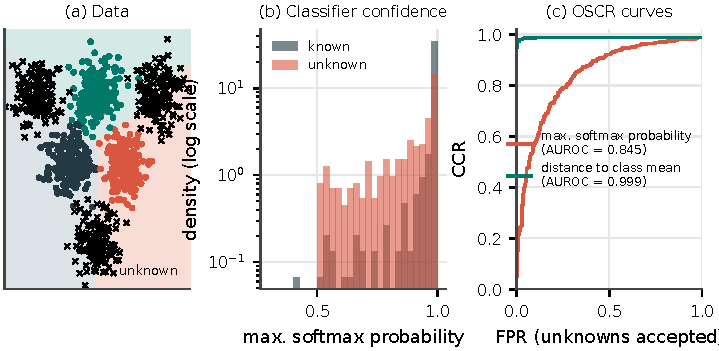
\includegraphics[width=\textwidth]{ch01/open_set}
\caption{Open-set recognition with three known classes. (a) Unknown examples (crosses) fall in
the regions of known classes. (b) The maximum softmax probability of the classifier is high
for many unknowns. (c) OSCR curves of two rejection scores.}
\label{fig:openset}
\end{figure}

In \cref{fig:openset} a logistic regression classifies the three known classes almost
perfectly (closed-set accuracy 0.988), but many unknowns receive a high confidence, and using
the maximum softmax probability to reject them gives an AUROC of only 0.845. A distance-based
score (minus the distance to the nearest class mean) separates them almost perfectly (0.999).
The main families of methods are:
\begin{itemize}
  \item \emph{confidence thresholding}: predict ``unknown'' if the highest class probability
        is below a threshold \citep{hendrycks2017baseline}. It is a simple baseline, but
        models, and deep networks in particular, are often overconfident: a network may say
        ``car: 99\%'' for an image of pure noise. ODIN \citep{liang2018enhancing} improves the
        separation with temperature scaling and small perturbations of the input;
  \item \emph{distance-based methods} (metric learning): the model maps the examples into a
        space where each class forms a compact cluster, and an example far from all clusters
        is rejected, for instance using the Mahalanobis distance \citep{lee2018simple};
  \item \emph{background class} or \emph{outlier exposure\index{outlier exposure|textbf}}: the model is trained with an
        auxiliary set of ``garbage'' examples labelled as unknown
        \citep{hendrycks2019deep}. It is very effective when the auxiliary data resemble the
        unknowns that will actually appear.
\end{itemize}

\begin{pitfall}
Open-set results depend heavily on which unknown classes are used for testing: a method that
rejects random noise easily may fail on unknowns that resemble the known classes. Always
describe the open-set protocol (known classes, unknown classes, their proportions).
\end{pitfall}

% ---------------------------------------------------------------------
\section{Evaluation in computer vision}\label{sec:vision}

\subsection{Tasks}

Computer vision distinguishes three main tasks. \emph{Image classification} assigns a single
label to a whole image (``what is in this image?'') and is evaluated with the metrics of
\cref{sec:crisp,sec:roc,sec:scoring,sec:calibration}, often with \emph{top-$k$ accuracy\index{accuracy|textbf}} (the
actual class is among the $k$ classes with the highest scores). \emph{Object detection\index{object detection|textbf}}
identifies what is in the image and \emph{where}: it draws a bounding box around each object
and labels it, as the YOLO family of detectors does \citep{redmon2016you,jocher2023yolov8}.
\emph{Image segmentation\index{segmentation|textbf}} classifies the image at the pixel level: \emph{semantic}
segmentation assigns a class to every pixel, \emph{instance} segmentation separates the
individual objects, and \emph{panoptic} segmentation does both; foundation models such as SAM
\citep{kirillov2023segment} segment arbitrary objects.

\subsection{Object detection: IoU, AP and mAP}

The \emph{intersection over union\index{intersection over union (IoU)|textbf}} (IoU, or Jaccard index) measures how well a predicted box
$B_p$ overlaps the ground-truth box $B_{gt}$:
\begin{equation}
  \mathrm{IoU}=\frac{\operatorname{area}(B_p\cap B_{gt})}{\operatorname{area}(B_p\cup B_{gt})}.
\end{equation}
An IoU of 1 is a perfect match. In \cref{fig:iou}a the boxes have areas 16 and 16 and an
intersection of 6, so $\mathrm{IoU}=6/26=0.231$. A detection counts as a true positive if it
has the same class as a ground-truth object, its IoU with it reaches a threshold (typically
0.5), and that object has not already been matched by a more confident detection; otherwise it
is a false positive (duplicates included). Ground-truth objects that are never matched are
false negatives.

\begin{figure}[htbp]
\centering
\begin{subfigure}[b]{0.46\textwidth}
\centering
\begin{tikzpicture}[scale=0.52,font=\footnotesize\sffamily]
  \draw[step=1,black!10,very thin] (0,0) grid (10,8);
  \fill[edmteal!35] (4,3) rectangle (6,6);
  \draw[edmnavy,very thick] (2,2) rectangle (6,6);
  \draw[edmcoral,very thick,dashed] (4,3) rectangle (8,7);
  \node[edmnavy,anchor=north] at (4,2) {ground truth $(2,2)$--$(6,6)$};
  \node[edmcoral,anchor=south] at (6,7) {prediction $(4,3)$--$(8,7)$};
  \node[edmteal!60!black] at (5,4.5) {$6$};
  \foreach \x in {0,2,...,10} \node[below,black!50,font=\tiny] at (\x,-0.9) {\x};
  \foreach \y in {0,2,...,8} \node[left,black!50,font=\tiny] at (0,\y) {\y};
\end{tikzpicture}
\caption{Two boxes: $\mathrm{IoU}=6/(16+16-6)=0.231$.}
\end{subfigure}\hfill
\begin{subfigure}[b]{0.46\textwidth}
\centering
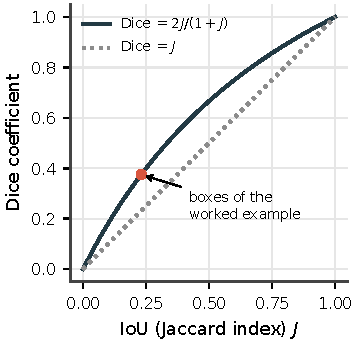
\includegraphics[width=0.9\textwidth]{ch01/dice_iou}
\caption{Dice coefficient against IoU.}
\end{subfigure}
\caption{Overlap measures. (a) Intersection over union of a predicted and a ground-truth box
(the intersection is shaded). (b) The Dice coefficient is a monotone function of the IoU and is
always at least as large.}
\label{fig:iou}
\end{figure}

Detections are sorted by confidence, and precision and recall are computed down the ranked
list. The \emph{average precision\index{average precision|textbf}\index{precision|textbf}} (AP) of a class is the area under its precision--recall
curve\index{precision--recall curve}, computed after replacing each precision by the maximum precision at any higher recall
(the \emph{interpolated} precision, which makes the curve monotone):
\begin{equation}
  \mathrm{AP}=\sum_k(r_k-r_{k-1})\,p_{\text{interp}}(r_k),\qquad
  p_{\text{interp}}(r)=\max_{r'\geq r}p(r').
\end{equation}
This all-point interpolation is used by PASCAL VOC since 2010; VOC 2007 averaged the
interpolated precision at 11 recall levels ($0,0.1,\dots,1$) and COCO uses 101 levels
\citep{everingham2010pascal,padilla2020survey}.

\begin{example}{Average precision of a detector}{ap}
A detector produces eight detections of class \emph{car}, sorted by confidence, in images that
contain five cars:
\begin{center}\small
\setlength{\tabcolsep}{5pt}
\begin{tabular}{@{}lcccccccc@{}}
\toprule
Rank & 1 & 2 & 3 & 4 & 5 & 6 & 7 & 8\\
Match (IoU $\geq0.5$) & TP & TP & FP & TP & FP & FP & TP & FP\\
Precision & 1.000 & 1.000 & 0.667 & 0.750 & 0.600 & 0.500 & 0.571 & 0.500\\
Recall & 0.2 & 0.4 & 0.4 & 0.6 & 0.6 & 0.6 & 0.8 & 0.8\\
\bottomrule
\end{tabular}
\end{center}
One car is never detected, so the maximum recall is 0.8. The interpolated precision is 1 up
to recall 0.4, $\max(0.750,0.600,0.500,0.571,0.500)=0.75$ at recall 0.6 and 0.571 at recall
0.8, so $\mathrm{AP}=0.2\cdot1+0.2\cdot1+0.2\cdot0.75+0.2\cdot0.571=0.664$
(\cref{fig:detectionpr} and \cref{lst:ap}). With the 11-point interpolation of VOC 2007, which averages the interpolated precision at the
recall levels $0,0.1,\dots,1$, the result would be approximately 0.695.
\end{example}

\begin{figure}[htbp]
\centering
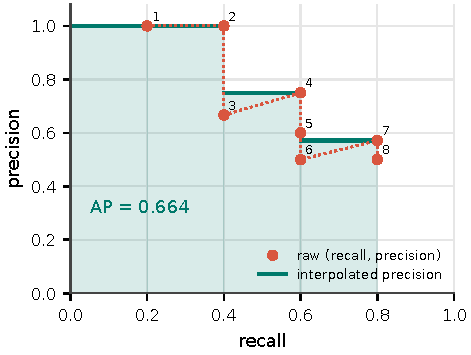
\includegraphics[width=0.56\textwidth]{ch01/detection_pr}
\caption{Precision--recall points of the detections of \cref{ex:ap} (numbered by rank),
interpolated precision and average precision (shaded area).}
\label{fig:detectionpr}
\end{figure}

\begin{pylisting}[label={lst:ap}]{IoU of two boxes and average precision of a ranked list of detections}
import numpy as np

def iou(a, b):
    """Intersection over union of two boxes given as (x1, y1, x2, y2)."""
    w = max(0, min(a[2], b[2]) - max(a[0], b[0]))
    h = max(0, min(a[3], b[3]) - max(a[1], b[1]))
    area = lambda r: (r[2] - r[0]) * (r[3] - r[1])
    return w * h / (area(a) + area(b) - w * h)

print(f"IoU = {iou((2, 2, 6, 6), (4, 3, 8, 7)):.3f}")

tp = np.array([1, 1, 0, 1, 0, 0, 1, 0])     # detections sorted by confidence
n_gt = 5                                    # number of ground-truth objects
prec = np.cumsum(tp) / np.arange(1, len(tp) + 1)
rec = np.cumsum(tp) / n_gt
env = np.maximum.accumulate(prec[::-1])[::-1]   # interpolated precision
ap = np.sum(np.diff(np.r_[0, rec]) * env)       # all-point interpolation
print("precision:", prec.round(3))
print("recall:   ", rec.round(2))
print(f"AP = {ap:.4f}")
\end{pylisting}
\begin{pyoutput}
IoU = 0.231
precision: [1.    1.    0.667 0.75  0.6   0.5   0.571 0.5  ]
recall:    [0.2 0.4 0.4 0.6 0.6 0.6 0.8 0.8]
AP = 0.6643
\end{pyoutput}

The \emph{mean average precision\index{mean average precision (mAP)|textbf}} (mAP) is the average of the AP over all classes (cars,
pedestrians, traffic lights\dots) and is the standard metric of detection benchmarks.
\emph{mAP@0.5} counts a detection as correct when its IoU exceeds 0.5 (PASCAL VOC), whereas
\emph{mAP@[0.5:0.95]} averages the mAP over IoU thresholds $0.50,0.55,\dots,0.95$ (COCO), so it
also rewards precise localisation \citep{lin2014microsoft}.

\subsection{Segmentation: pixel accuracy, mIoU and Dice}

\emph{Pixel accuracy\index{accuracy|textbf}}, the percentage of correctly classified pixels, suffers from the same
problem as accuracy with imbalanced\index{class imbalance} classes: if 90\% of an image is sky, a model that always
predicts ``sky'' reaches 90\% pixel accuracy while failing completely on the road and the cars.
The \emph{mean intersection over union\index{intersection over union (IoU)|textbf}} (mIoU) computes the IoU of each class at pixel level,
$\TP_j/(\TP_j+\FP_j+\FN_j)$, and averages it over classes \citep{long2015fully}, which prevents
large background classes from hiding errors on small but important classes such as
pedestrians.

The \emph{Dice\index{Dice coefficient|textbf} coefficient} \citep{dice1945measures} is the $F_1$ score at pixel level:
\begin{equation}
  \mathrm{Dice}=\frac{2|A\cap B|}{|A|+|B|}=\frac{2\TP}{2\TP+\FP+\FN}.
\end{equation}
It is very common in medical imaging (for instance, to segment a tumour). Dice and IoU treat
false positives and false negatives in the same, symmetric way; the difference is that Dice
counts the overlap twice, so for the same errors Dice is larger than IoU. In fact
$\mathrm{Dice}=2J/(1+J)$ with $J$ the IoU (\cref{fig:iou}b): the two boxes of \cref{fig:iou}a,
seen as masks, have $\mathrm{IoU}=0.231$ and $\mathrm{Dice}=0.375$. Being monotonically related,
they rank the segmentations\index{segmentation} of a single image identically, but their averages over many images
can rank models differently. When the shape of the boundary matters, distance-based metrics such
as the Hausdorff distance are used \citep{taha2015metrics}; \citet{maierhein2024metrics} give
detailed guidelines for choosing metrics in image analysis.

% ---------------------------------------------------------------------
\section{Evaluation in natural language processing}\label{sec:nlp}

The choice of metric in natural language processing (NLP) depends above all on whether the
model performs a \emph{classification} task (sentiment analysis, topic labelling, named entity
recognition) or a \emph{generation} task (translation, summarisation, dialogue).

\subsection{Classification and labelling tasks}

When an NLP model outputs a class (positive or negative sentiment, a topic, an intent), the
metrics of \cref{sec:crisp} apply: accuracy for balanced problems, and per-class precision,
recall and $F_1$ otherwise. In \emph{named entity recognition} most tokens belong to the
non-entity class ``O'', so token accuracy is uninformative; the standard is entity-level $F_1$,
where an entity counts as correct only if both its span and its type match exactly
\citep{tjong2003introduction}. Cohen's kappa\index{Cohen's kappa} is used to measure the agreement between human
annotators and thus the reliability of the data set.

\subsection{Text generation: n-gram overlap metrics}

Evaluating generated text is difficult because there is no single correct answer: the same
sentence can be translated or summarised in many valid ways. Traditional metrics compare the
output of the model with one or more human-written \emph{references} by counting shared
$n$-grams (sequences of $n$ words).

BLEU\index{BLEU} \citep{papineni2002bleu}, designed for machine translation, focuses on precision. For each
$n$ it computes the \emph{modified} $n$-gram precision $p_n$, in which each $n$-gram of the
candidate is counted at most as many times as it appears in the reference, and combines them
with a geometric mean and a \emph{brevity penalty} BP that prevents very short candidates from
obtaining high precision:
\begin{equation}
  \mathrm{BLEU}=\mathrm{BP}\cdot\exp\Bigl(\sum_{n=1}^{N}w_n\log p_n\Bigr),
  \qquad
  \mathrm{BP}=\begin{cases}1 & \text{if } \ell_c>\ell_r,\\ e^{1-\ell_r/\ell_c} & \text{otherwise,}\end{cases}
\end{equation}
where $\ell_c$ and $\ell_r$ are the lengths of the candidate and the reference, and usually
$N=4$ and $w_n=1/4$.

\begin{example}{BLEU and ROUGE by hand}{bleu}
Let the reference be ``\emph{the cat is on the mat}''. Candidate A, ``\emph{the cat sat on the
mat}'', has modified precisions $p_1=5/6$, $p_2=3/5$ (\emph{the cat}, \emph{on the},
\emph{the mat}), $p_3=1/4$ and $p_4=0$, and the same length as the reference. Its BLEU-4 is 0,
because one of the precisions is zero: at sentence level BLEU needs smoothing
\citep{chen2014systematic}, and it was designed to be computed over a whole corpus. Its BLEU-2
(only unigrams and bigrams) is $\sqrt{5/6\cdot3/5}=0.707$.

Candidate B, ``\emph{the feline is on the rug}'', means exactly the same as the reference but
uses synonyms: $p_1=4/6$, $p_2=2/5$ and BLEU-2 $=\sqrt{4/6\cdot2/5}=0.516$. BLEU does not
understand synonyms. Its ROUGE\index{ROUGE}-1 recall is also $4/6=0.667$, and the longest common subsequence
with the reference, ``\emph{the is on the}'', has four words, so ROUGE-L recall and precision
are $4/6$ as well.
\end{example}

Several metrics address the limitations of BLEU:
\begin{itemize}
  \item METEOR\index{METEOR} \citep{banerjee2005meteor} aligns the words of candidate and reference using
        exact matches, stems (\emph{running} matches \emph{run}) and synonyms from WordNet,
        combines precision and recall (weighting recall more) and penalises differences in word
        order;
  \item ROUGE \citep{lin2004rouge}, designed for summarisation, focuses on recall: ROUGE-N is
        the fraction of the reference $n$-grams that appear in the candidate (how much of the
        reference summary the model captured), and ROUGE-L is based on the longest common
        subsequence;
  \item chrF \citep{popovic2015chrf} computes an F-score\index{F1 score@$F_1$ score} over character $n$-grams, which is
        more robust to morphology.
\end{itemize}

\subsection{Embedding-based and learned metrics}

Modern metrics use neural representations to check whether the \emph{meaning} is the same, even
when the words differ. BERTScore\index{BERTScore} \citep{zhang2020bertscore} represents each token of the
candidate $\hat x$ and of the reference $x$ by its contextual embedding\index{embedding} and matches each token
with its most similar token in the other sentence; for instance, the recall is
\begin{equation}
  R_{\text{BERT}}=\frac{1}{|x|}\sum_{x_i\in x}\ \max_{\hat x_j\in\hat x}\ \mathbf x_i^{\top}\hat{\mathbf x}_j,
\end{equation}
with normalised embeddings, so that the inner product is the cosine\index{cosine similarity} similarity\index{similarity measure}. ``Cat'' and
``feline'' obtain a high similarity. \emph{Learned} metrics such as COMET \citep{rei2020comet} go
further and are trained to predict human quality judgements. These metrics correlate better with
human judgement than $n$-gram overlap, at the price of interpretability\index{interpretability} and of inheriting the
biases of the underlying models.

\subsection{Language models and LLMs}

A language model\index{language model} is evaluated intrinsically by its \emph{perplexity} on held-out text,
\begin{equation}
  \mathrm{PPL}=\exp\Bigl(-\frac1N\sum_{t=1}^{N}\log p(w_t\mid w_{<t})\Bigr),
\end{equation}
which is the exponential of the per-token log loss\index{log loss} of \cref{sec:scoring}. A model that assigns
probability $1/4$ to every token has perplexity 4: it is as uncertain as if it had to choose
among four equally likely words. Perplexities are only comparable for the same tokenisation and
test text.

For large language models\index{large language model (LLM)} (LLMs), traditional metrics often fail, because a correct answer may
look nothing like the reference. Common approaches are:
\begin{itemize}
  \item \emph{benchmarks} with automatically checkable answers, such as multiple-choice
        questions \citep[e.g.][]{hendrycks2021measuring}, evaluated with accuracy;
  \item \emph{functional correctness} for code: the generated program is run against unit
        tests\index{testing!unit tests}. The metric pass@$k$ is the probability that at least one of $k$ generated
        samples passes; with $n\geq k$ samples of which $c$ pass, an unbiased estimator is
        $1-\binom{n-c}{k}\big/\binom{n}{k}$ \citep{chen2021evaluating}. With $n=10$ and $c=3$,
        pass@1 $=0.3$ and pass@5 $=1-21/252=0.917$;
  \item \emph{LLM-as-a-judge\index{LLM-as-a-judge|textbf}} \citep{zheng2023judging}: a stronger model grades the outputs of
        another, either scoring each answer against a rubric (``rate this answer from 1 to 5
        according to its helpfulness'') or comparing two answers. It is cheap and agrees
        reasonably well with humans, but judges have known biases: \emph{position} bias
        (preferring the first or the second answer), \emph{verbosity} bias (preferring longer
        answers) and \emph{self-enhancement} bias (preferring answers produced by
        themselves). Mitigations include swapping the order of the answers, using explicit
        rubrics or reference answers \citep{liu2023geval}, and validating the judge against a
        sample of human judgements (reporting, for instance, Cohen's kappa\index{Cohen's kappa});
  \item \emph{human preference} evaluation: platforms such as Chatbot Arena collect pairwise
        votes and aggregate them with Bradley--Terry or Elo-style models
        \citep{chiang2024chatbot}.
\end{itemize}
Finally, benchmark questions may have leaked into the enormous pre-training corpora
(\emph{data contamination\index{contamination of benchmarks|textbf}}), which inflates the scores: this is data leakage\index{data leakage}
(\cref{sec:protocols}) at the scale of the Internet. Recent or private test sets are preferable.

\subsection{Retrieval-augmented generation}

A retrieval-augmented generation\index{retrieval-augmented generation (RAG)} (RAG) system first retrieves documents relevant to a question
and then generates an answer conditioned on them. Both components must be evaluated. The
\emph{retrieval} step is evaluated with ranking metrics (recall@$k$, MRR\index{mean reciprocal rank}, NDCG\index{NDCG}) or with
\emph{context precision\index{precision|textbf}} (are the retrieved passages relevant?) and \emph{context recall\index{recall|textbf}} (do
they contain the information needed?). The \emph{generation} step is evaluated with
\emph{faithfulness\index{faithfulness|textbf}} (is every claim of the answer supported by the retrieved documents, that is,
are there no hallucinations?), \emph{answer relevance} (does the answer actually address the
question?) and, when a reference answer exists, correctness. Frameworks such as RAGAS
\citep{es2024ragas} compute these quantities with LLM\index{large language model (LLM)} judges; for instance, faithfulness is the
fraction of the statements of the answer that can be inferred from the retrieved context.

% ---------------------------------------------------------------------
\section{Evaluating unsupervised models}\label{sec:unsupervised}

\subsection{The absence of ground truth}

Unsupervised models look for patterns in the data: groups of similar examples, associations
between variables, low-dimensional structure. Evaluating them is harder than evaluating
supervised models for two reasons. First, the patterns found may not genuinely exist: $k$-means
returns $k$ clusters even when applied to uniform noise. Second, there is no ``ground truth'',
no set of reference answers on which to test hypotheses. Unsupervised models are therefore
compared by how well they fit the data (\emph{internal} evaluation), by their agreement with
external information when it is available (\emph{external} evaluation), by their stability
when the data are perturbed \citep{vonluxburg2010clustering}, and ultimately by their usefulness
for the task that motivated the analysis.

\subsection{Clustering: internal evaluation}

Internal evaluation judges a clustering\index{clustering} using only the data that were clustered. The most
popular indices reward compact and well-separated clusters.

The \emph{silhouette\index{silhouette coefficient|textbf} coefficient} \citep{rousseeuw1987silhouettes} is computed for each example
$i$ from two quantities: $a(i)$, the mean distance between $i$ and the other points of its
cluster, and $b(i)$, the mean distance between $i$ and the points of the nearest other cluster:
\begin{equation}
  s(i)=\frac{b(i)-a(i)}{\max\{a(i),b(i)\}}\in[-1,1].
\end{equation}
The coefficient of a clustering is the mean of $s(i)$ over all the examples. Values close to 1
indicate dense, well-separated clusters, values around zero indicate overlapping clusters, and
negative values suggest that examples have been assigned to the wrong cluster. \emph{Silhouette
plots} show the individual values sorted within each cluster (\cref{fig:silhouette}): with
$k=4$, the true number of groups in the data, all the clusters are thick and have high values
(mean 0.772); with $k=3$ two groups are merged (0.740); with $k=5$ one group is split into two
thin clusters with low silhouettes (0.648).

\begin{figure}[htbp]
\centering
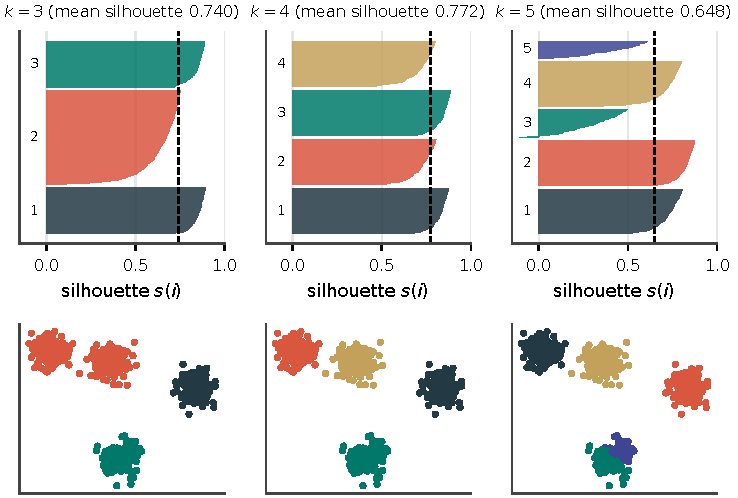
\includegraphics[width=\textwidth]{ch01/silhouette}
\caption{Silhouette plots (top) and $k$-means clusterings (bottom) of 600 points generated from
four groups, for $k=3,4,5$. The dashed line marks the mean silhouette.}
\label{fig:silhouette}
\end{figure}

The \emph{Calinski--Harabasz\index{Calinski--Harabasz index|textbf} index} (or variance ratio criterion) \citep{calinski1974dendrite}
is the ratio between the dispersion \emph{between} clusters and the dispersion \emph{within}
clusters, each normalised by its degrees of freedom:
\begin{equation}
  \mathrm{CH}=\frac{\operatorname{tr}(B_k)/(k-1)}{\operatorname{tr}(W_k)/(n-k)},
  \quad
  B_k=\sum_{q=1}^{k}n_q(\mathbf c_q-\mathbf c)(\mathbf c_q-\mathbf c)^{\top},
  \quad
  W_k=\sum_{q=1}^{k}\sum_{x\in C_q}(x-\mathbf c_q)(x-\mathbf c_q)^{\top},
\end{equation}
where $\mathbf c_q$ and $n_q$ are the centroid and size of cluster $C_q$ and $\mathbf c$ is the
global centroid; the traces are sums of squared distances. The score is higher when clusters are
dense and well separated, and it is fast to compute.

The \emph{Davies--Bouldin\index{Davies--Bouldin index|textbf} index} \citep{davies1979cluster} estimates the average similarity\index{similarity measure}
between each cluster and its most similar one, where similarity compares the distance between
clusters with their sizes:
\begin{equation}
  \mathrm{DB}=\frac1k\sum_{i=1}^{k}\max_{j\neq i}\frac{\sigma_i+\sigma_j}{d(\mathbf c_i,\mathbf c_j)},
\end{equation}
with $\sigma_i$ the mean distance of the points of cluster $i$ to its centroid. Lower values are
better (the minimum is 0). It is simpler to compute than the silhouette, but it is based on
centroids and therefore limited to Euclidean\index{Euclidean distance} distance.

In \cref{fig:indices} and \cref{lst:clustering} the three indices agree on $k=4$. In general
they do not always agree, and all of them favour convex, compact clusters: their values are generally
more favourable (higher for silhouette and Calinski--Harabasz, lower for Davies--Bouldin) for
$k$-means-like partitions than for other notions of cluster, such as the
density-based clusters found by DBSCAN, and they can be misleading for elongated or nested
shapes. The ``elbow'' of the within-cluster sum of squares is a common heuristic, and the
\emph{gap statistic} \citep{tibshirani2001estimating} compares it with what would be expected
for data without clusters.

\begin{figure}[htbp]
\centering
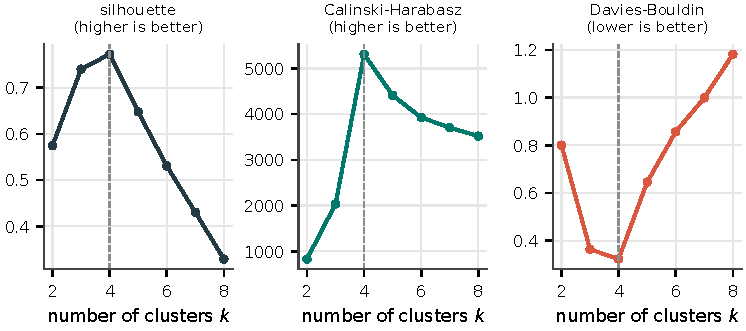
\includegraphics[width=\textwidth]{ch01/internal_indices}
\caption{Internal indices for $k$-means with $k=2,\dots,8$ on the data of \cref{fig:silhouette}.
All three point to $k=4$ (dashed lines).}
\label{fig:indices}
\end{figure}

\begin{pylisting}[label={lst:clustering}]{Internal and external indices for k-means with k = 2..6}
from sklearn.cluster import KMeans
from sklearn.datasets import make_blobs
from sklearn.metrics import (silhouette_score, calinski_harabasz_score,
                             davies_bouldin_score, adjusted_rand_score,
                             normalized_mutual_info_score)

X, y = make_blobs(n_samples=600, centers=4, cluster_std=1.2, random_state=7)
for k in range(2, 7):
    lab = KMeans(n_clusters=k, n_init=10, random_state=0).fit_predict(X)
    print(f"k={k}  sil={silhouette_score(X, lab):.3f}  "
          f"CH={calinski_harabasz_score(X, lab):6.0f}  "
          f"DB={davies_bouldin_score(X, lab):.3f}  "
          f"ARI={adjusted_rand_score(y, lab):.3f}  "
          f"NMI={normalized_mutual_info_score(y, lab):.3f}")
\end{pylisting}
\begin{pyoutput}
k=2  sil=0.574  CH=   832  DB=0.801  ARI=0.495  NMI=0.657
k=3  sil=0.740  CH=  2036  DB=0.364  ARI=0.713  NMI=0.857
k=4  sil=0.772  CH=  5309  DB=0.323  ARI=1.000  NMI=1.000
k=5  sil=0.648  CH=  4410  DB=0.646  ARI=0.918  NMI=0.944
k=6  sil=0.531  CH=  3926  DB=0.857  ARI=0.824  NMI=0.891
\end{pyoutput}

\subsection{Clustering: external evaluation}

When reference labels exist (for benchmarking, or for a labelled subset of the data), the
clustering\index{clustering} can be compared with them. Since cluster identifiers are arbitrary, the measures
must be invariant to permutations of the labels:
\begin{itemize}
  \item the \emph{Rand index} \citep{rand1971objective} is the fraction of pairs of examples
        on which both partitions agree (both together or both apart). The \emph{adjusted Rand
        index\index{adjusted Rand index|textbf}} (ARI) \citep{hubert1985comparing} corrects it for chance,
        $\mathrm{ARI}=(\mathrm{RI}-\E[\mathrm{RI}])/(\max\mathrm{RI}-\E[\mathrm{RI}])$: it is 1
        for identical partitions, close to 0 for random ones and can be negative;
  \item the \emph{mutual information} (MI) between the two labellings measures their agreement
        ignoring permutations. Its \emph{normalised} version (NMI\index{normalised mutual information}) \citep{strehl2002cluster}
        lies in $[0,1]$ and is very popular, but it is not corrected for chance and tends to
        increase with the number of clusters; the \emph{adjusted} mutual information (AMI)
        corrects it \citep{vinh2010information};
  \item \emph{homogeneity} (each cluster contains members of a single class),
        \emph{completeness} (all members of a class are assigned to the same cluster) and their
        harmonic mean, the \emph{V-measure} \citep{rosenberg2007vmeasure}, make the two kinds
        of error explicit.
\end{itemize}

\subsection{Association rules}

\emph{Association rule\index{association rules|textbf}} learning discovers interesting relations between variables in large
databases \citep{agrawal1993mining}. It identifies strong rules, ranked by some measure of
interestingness, and is used in market basket analysis, web usage mining, intrusion detection
and bioinformatics. A rule $A\Rightarrow B$ has an \emph{antecedent} $A$ and a
\emph{consequent} $B$, two disjoint sets of items. Unlike classification rules, any attribute can
appear in the consequent, and it can contain more than one attribute. \Cref{tab:baskets} shows
ten shopping baskets, and we evaluate the rule
\begin{center}
\textsc{if} sponge cakes ``Goloso'' $=1$ \textsc{and} horchata ``Xufer'' $=1$
\textsc{then} biscuits ``Trigo'' $=1$.
\end{center}

\begin{table}[htbp]
\centering\small
\caption{Ten shopping baskets (1 = the product was bought).}\label{tab:baskets}
\setlength{\tabcolsep}{4.5pt}
\begin{tabular}{@{}lccccccc@{}}
\toprule
& \makecell{Wine\\``Cabez\'on''} & \makecell{Soda\\``Chispa''} & \makecell{Wine\\``T\'io Paco''}
& \makecell{Horchata\\``Xufer''} & \makecell{Sponge cakes\\``Goloso''} & \makecell{Biscuits\\``Trigo''}
& \makecell{Chocolate\\``La Vaca''}\\
\midrule
T1  & 1 & 1 & 0 & 0 & 0 & 1 & 0\\
T2  & 0 & 1 & 1 & 0 & 0 & 0 & 0\\
T3  & 0 & 0 & 0 & 1 & 1 & 1 & 0\\
T4  & 1 & 1 & 0 & 1 & 1 & 1 & 1\\
T5  & 0 & 0 & 0 & 0 & 0 & 1 & 0\\
T6  & 1 & 0 & 0 & 0 & 0 & 1 & 1\\
T7  & 0 & 1 & 1 & 1 & 1 & 0 & 0\\
T8  & 0 & 0 & 0 & 1 & 1 & 1 & 1\\
T9  & 1 & 1 & 0 & 0 & 1 & 0 & 1\\
T10 & 0 & 1 & 0 & 0 & 1 & 0 & 0\\
\bottomrule
\end{tabular}
\end{table}

The usual measures are:
\begin{itemize}
  \item \emph{support}: how frequently the itemset $A\cup B$ (all the items of the rule) appears
        in the data. In probabilistic terms it is $P(A\cap B)$, the probability that a
        transaction contains $A$ \emph{and} $B$; some texts write $P(A\cup B)$ meaning the
        union of the \emph{itemsets}, which can be confusing. Three baskets (T3, T4, T8) contain
        the three products: absolute support 3, relative support $3/10=0.3$;
  \item \emph{confidence}: how frequently the rule is true when it can be applied,
        $P(B\mid A)=\mathrm{supp}(A\cup B)/\mathrm{supp}(A)$. Four baskets contain $A$ (T3, T4,
        T7, T8), so the confidence is $3/4=0.75$;
  \item \emph{lift\index{lift|textbf}} \citep{brin1997dynamic}: the ratio between the observed support and the
        support expected if $A$ and $B$ were independent,
        $\mathrm{conf}(A\Rightarrow B)/P(B)=P(A\cap B)/\bigl(P(A)P(B)\bigr)$. Six baskets contain
        $B$, so $\mathrm{lift}=0.3/(0.4\cdot0.6)=1.25$. A lift of 1 means independence; above 1,
        the presence of $A$ increases the probability of $B$; below 1, it decreases it;
  \item \emph{leverage}, $P(A\cap B)-P(A)P(B)=0.06$, and \emph{conviction\index{conviction|textbf}},
        $(1-P(B))/(1-\mathrm{conf})=0.4/0.25=1.6$, which is infinite for rules that are always
        true.
\end{itemize}

\begin{pylisting}[label={lst:assoc}]{Interestingness measures of an association rule}
import pandas as pd

items = ["Cabezon", "Chispa", "TioPaco", "Xufer", "Goloso", "Trigo", "LaVaca"]
T = pd.DataFrame([[1, 1, 0, 0, 0, 1, 0], [0, 1, 1, 0, 0, 0, 0], [0, 0, 0, 1, 1, 1, 0],
                  [1, 1, 0, 1, 1, 1, 1], [0, 0, 0, 0, 0, 1, 0], [1, 0, 0, 0, 0, 1, 1],
                  [0, 1, 1, 1, 1, 0, 0], [0, 0, 0, 1, 1, 1, 1], [1, 1, 0, 0, 1, 0, 1],
                  [0, 1, 0, 0, 1, 0, 0]], columns=items).astype(bool)

A = T["Goloso"] & T["Xufer"]          # antecedent: {Goloso, Xufer}
B = T["Trigo"]                        # consequent: {Trigo}
supp = (A & B).mean()
conf = supp / A.mean()
lift = conf / B.mean()
leverage = supp - A.mean() * B.mean()
conviction = (1 - B.mean()) / (1 - conf)
print(f"support={supp:.2f} confidence={conf:.2f} lift={lift:.2f} "
      f"leverage={leverage:.2f} conviction={conviction:.2f}")
\end{pylisting}
\begin{pyoutput}
support=0.30 confidence=0.75 lift=1.25 leverage=0.06 conviction=1.60
\end{pyoutput}

Two cautions apply. A high confidence can be misleading when the consequent is very frequent:
if 90\% of the baskets contain bread, a rule predicting bread with confidence 0.8 has a lift
below 1, so its antecedent actually makes bread \emph{less} likely. And when thousands of rules
are generated, many will look interesting by chance, so promising rules should be validated on
new data \citep{tan2004selecting,han2011data}.

\subsection{Other unsupervised tasks}

In \emph{anomaly detection} \citep{chandola2009anomaly}, if some labelled anomalies are
available the problem is evaluated as an extremely imbalanced\index{class imbalance} classification problem (AUC,
average precision\index{average precision}, precision@$k$ among the top-ranked cases); otherwise, experts review the
top-ranked anomalies. \emph{Dimensionality reduction} can be evaluated by the reconstruction
error, by how well neighbourhoods are preserved, or by the performance of a downstream model.
Density estimators and generative models are evaluated by the log-likelihood of held-out data,
the log loss\index{log loss} once again.

% ---------------------------------------------------------------------
\section{Comparing models statistically}\label{sec:stats}

Every performance estimate is a random variable: a different test set or a different partition
in cross-validation would give a different number. Before concluding that model A is better than
model B, we must ask whether the difference could be due to chance.

\subsection{Uncertainty of a single estimate}

If a classifier is tested on $n$ independent examples, the number of correct predictions follows
a binomial distribution. The \emph{Wilson\index{Wilson interval|textbf} interval} \citep{wilson1927probable} for the accuracy
$\hat p$ behaves better than the usual normal approximation $\hat p\pm z\sqrt{\hat p(1-\hat p)/n}$,
especially for small $n$ or accuracies close to 1:
\begin{equation}
  \frac{\hat p+\frac{z^2}{2n}\pm z\sqrt{\frac{\hat p(1-\hat p)}{n}+\frac{z^2}{4n^2}}}{1+\frac{z^2}{n}},
\end{equation}
with $z=1.96$ for 95\% confidence. An accuracy of 170/200 has the interval $[0.794, 0.893]$. For
metrics without a simple sampling distribution (AUC, $F_1$, MCC\index{Matthews correlation coefficient}\dots) the \emph{bootstrap\index{bootstrap|textbf}}
\citep{efron1993introduction} is the general solution: resample the test set with replacement
many times, recompute the metric on each resample and take the percentiles of the results
(\cref{lst:ci}).

\begin{pylisting}[label={lst:ci}]{Wilson interval for accuracy and bootstrap interval for the AUC}
import numpy as np
from scipy.stats import norm
from sklearn.metrics import roc_auc_score

def wilson_ci(k, n, conf=0.95):
    """Wilson score interval for a proportion (e.g. accuracy = k/n)."""
    z, p = norm.ppf(0.5 + conf / 2), k / n
    centre = (p + z**2 / (2 * n)) / (1 + z**2 / n)
    half = z * np.sqrt(p * (1 - p) / n + z**2 / (4 * n**2)) / (1 + z**2 / n)
    return centre - half, centre + half

def bootstrap_ci(metric, y, s, B=2000, conf=0.95, seed=0):
    """Percentile bootstrap interval for any metric(y, s)."""
    rng, stats = np.random.default_rng(seed), []
    while len(stats) < B:
        i = rng.integers(0, len(y), len(y))
        if y[i].min() != y[i].max():          # the resample needs both classes
            stats.append(metric(y[i], s[i]))
    return np.quantile(stats, [(1 - conf) / 2, (1 + conf) / 2])

print("accuracy 170/200 = 0.850, 95%% Wilson CI: [%.3f, %.3f]" % wilson_ci(170, 200))
rng = np.random.default_rng(1)
y = np.r_[np.ones(60), np.zeros(140)]
s = np.r_[rng.normal(1.2, 1, 60), rng.normal(0, 1, 140)]
lo, hi = bootstrap_ci(roc_auc_score, y, s)
print(f"AUC = {roc_auc_score(y, s):.3f}, 95% bootstrap CI: [{lo:.3f}, {hi:.3f}]")
\end{pylisting}
\begin{pyoutput}
accuracy 170/200 = 0.850, 95% Wilson CI: [0.794, 0.893]
AUC = 0.843, 95% bootstrap CI: [0.779, 0.898]
\end{pyoutput}

\subsection{Two models on the same data}

When two classifiers are evaluated on the same test set, their errors are paired. \emph{McNemar\index{McNemar's test|textbf}'s
test} \citep{mcnemar1947note} uses only the examples on which they disagree: $b$, the number
correctly classified by A and misclassified by B, and $c$, the number misclassified by A and
correctly classified by B. If both models have the same error rate\index{error rate}, $b$ should follow a binomial
distribution $\mathrm{Bin}(b+c,1/2)$, which gives an exact test; for large counts,
$\chi^2=(|b-c|-1)^2/(b+c)$ with one degree of freedom is used. \citet{dietterich1998approximate}
recommends this test when the models can be trained only once.

With cross-validation, the tempting approach is a paired $t$-test on the $k$ fold differences.
It is not valid: the training sets overlap, the differences are positively correlated, the
variance is underestimated and the test finds far too many ``significant'' differences
\citep{dietterich1998approximate}. The \emph{corrected resampled\index{corrected resampled t-test@corrected resampled $t$-test|textbf} $t$-test}
\citep{nadeau2003inference} inflates the variance to account for the overlap:
\begin{equation}
  t=\frac{\bar d}{\sqrt{\Bigl(\frac1J+\frac{n_{\text{test}}}{n_{\text{train}}}\Bigr)\hat\sigma_d^2}},
\end{equation}
where $\bar d$ and $\hat\sigma_d^2$ are the mean and the variance of the $J$ differences, and
$n_{\text{test}}/n_{\text{train}}=1/(k-1)$ in $k$-fold CV. \Cref{lst:compare} compares logistic
regression and naive Bayes\index{naive Bayes}. McNemar's test finds no significant difference ($p=0.58$). Over
10$\times$10-fold CV the mean difference in accuracy is 0.015; the naive $t$-test declares it
overwhelmingly significant ($p\approx10^{-7}$), whereas the corrected test does not ($p=0.11$).

\begin{pylisting}[label={lst:compare}]{McNemar's test and the corrected resampled t-test}
import numpy as np
from scipy.stats import binomtest, t
from sklearn.datasets import make_classification
from sklearn.linear_model import LogisticRegression
from sklearn.model_selection import (RepeatedStratifiedKFold, cross_val_score,
                                     train_test_split)
from sklearn.naive_bayes import GaussianNB

X, y = make_classification(n_samples=2000, n_features=20, n_informative=5,
                           random_state=1)
A, B = LogisticRegression(max_iter=1000), GaussianNB()

# McNemar's exact test on a single test set
X_tr, X_te, y_tr, y_te = train_test_split(X, y, test_size=0.3, random_state=0)
ok_a = A.fit(X_tr, y_tr).predict(X_te) == y_te
ok_b = B.fit(X_tr, y_tr).predict(X_te) == y_te
b, c = np.sum(ok_a & ~ok_b), np.sum(~ok_a & ok_b)
print(f"McNemar: b={b}, c={c}, exact p-value = {binomtest(b, b + c).pvalue:.4f}")

# Corrected resampled t-test (Nadeau & Bengio, 2003) on 10 x 10-fold CV
cv = RepeatedStratifiedKFold(n_splits=10, n_repeats=10, random_state=0)
d = cross_val_score(A, X, y, cv=cv) - cross_val_score(B, X, y, cv=cv)
J, ratio = len(d), 1 / 9                  # n_test / n_train in 10-fold CV
t_c = d.mean() / np.sqrt((1 / J + ratio) * d.var(ddof=1))
t_naive = d.mean() / np.sqrt(d.var(ddof=1) / J)
print(f"mean difference = {d.mean():.4f}")
print(f"naive t = {t_naive:.2f} (p = {2 * t.sf(abs(t_naive), J - 1):.1e})")
print(f"corrected t = {t_c:.2f} (p = {2 * t.sf(abs(t_c), J - 1):.4f})")
\end{pylisting}
\begin{pyoutput}
McNemar: b=38, c=44, exact p-value = 0.5811
mean difference = 0.0150
naive t = 5.69 (p = 1.3e-07)
corrected t = 1.63 (p = 0.1055)
\end{pyoutput}

\subsection{Many models on many data sets}

To compare learning algorithms rather than models, they must be evaluated on many data sets.
\citet{demsar2006statistical} recommends non-parametric tests, which do not assume normality and
are not dominated by a few data sets:
\begin{itemize}
  \item for two algorithms, the \emph{Wilcoxon\index{Mann--Whitney--Wilcoxon statistic|textbf} signed-rank test} \citep{wilcoxon1945individual}
        on the differences of performance across data sets;
  \item for $k$ algorithms on $N$ data sets, the \emph{Friedman test\index{Friedman test|textbf}} \citep{friedman1937use}:
        the algorithms are ranked on each data set (1 for the best), $R_j$ is the average rank
        of algorithm $j$, and
        \begin{equation}
          \chi^2_F=\frac{12N}{k(k+1)}\Bigl[\sum_{j}R_j^2-\frac{k(k+1)^2}{4}\Bigr]
        \end{equation}
        follows approximately a $\chi^2$ distribution with $k-1$ degrees of freedom. If the
        null hypothesis is rejected, the \emph{Nemenyi\index{Nemenyi test|textbf}} post-hoc test declares two algorithms
        different if their average ranks differ by at least the \emph{critical difference\index{critical difference diagram|textbf}}
        $\mathrm{CD}=q_\alpha\sqrt{k(k+1)/(6N)}$, with $q_{0.05}=2.728$ for $k=5$.
\end{itemize}
The results are summarised in a \emph{critical difference diagram} (\cref{fig:cd}), which
places the algorithms on the axis of average ranks and joins with a bar the groups whose
differences are not significant.

\begin{figure}[htbp]
\centering
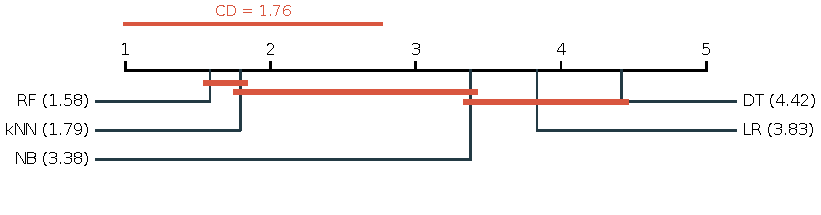
\includegraphics[width=\textwidth]{ch01/cd_diagram}
\caption{Critical difference diagram of five algorithms evaluated with the AUC (5-fold CV) on
12 synthetic data sets. Average ranks in parentheses; algorithms joined by a bar are not
significantly different (Nemenyi test, $\alpha=0.05$).}
\label{fig:cd}
\end{figure}

In the experiment of \cref{fig:cd}, logistic regression (LR), naive Bayes\index{naive Bayes} (NB), $k$-NN, a
decision tree (DT) and a random forest (RF) were compared on 12 data sets. The average ranks are
1.58 (RF), 1.79 ($k$-NN), 3.38 (NB), 3.83 (LR) and 4.42 (DT); the Friedman statistic is
$\chi^2_F=30.4$ ($p=4\times10^{-6}$) and $\mathrm{CD}=1.76$. Random forest and $k$-NN are
significantly better than logistic regression and the decision tree, and random forest is also
better than naive Bayes (difference 1.80), but $k$-NN and naive Bayes are not significantly
different (1.59). These conclusions depend on the data sets chosen: logistic regression ranks
low partly because two of the data sets (concentric circles) are not linearly separable.

Post-hoc tests on mean ranks, such as Nemenyi's, have a weakness: whether two algorithms are declared different
depends on which other algorithms take part in the comparison \citep{benavoli2016should}. When one method is the
reference (a new proposal, or the model in production), a safer analysis compares it with each of the others
using the Wilcoxon signed-rank test on the per-data-set differences \citep{wilcoxon1945individual}, with Holm's
step-down correction for the multiple comparisons \citep{holm1979simple}. Against random forest, the adjusted
$p$-values are 0.002 for LR and DT, 0.005 for NB and 0.077 for $k$-NN: the same conclusions as above, reached
without depending on the rest of the pool.

\citet{benavoli2017time} argue for \emph{Bayesian} comparisons, which give the posterior
probabilities that one algorithm is better, practically equivalent (within a \emph{region of
practical equivalence}) or worse than another: this is the question practitioners actually
want answered. With the Bayesian signed-rank test and a region of, say, $\pm0.01$ in AUC, the result is the
posterior probability of each of the three outcomes rather than a $p$-value.

\subsection{Statistical versus practical significance}

Statistical significance\index{statistical significance} is not practical significance. With a test set of a million examples a
difference of 0.1\% in accuracy can be significant and irrelevant; with 100 examples a
difference of 5\% may not be significant and yet be important. Report effect sizes with their
intervals, correct for multiple comparisons when many models are compared, and decide with the
costs and the context in mind. A model that wins on benchmark data sets may not win in your
deployment context.

% ---------------------------------------------------------------------
\section{Choosing the right metric}\label{sec:choosing}

There is no universally best metric. \Cref{tab:choosing} summarises the recommendations of this
unit, and the following questions help to design an evaluation:
\begin{enumerate}
  \item What decision will the model support: a crisp decision, a ranking or prioritisation, a
        probability estimate, a numerical forecast, a set or interval?
  \item Who bears the consequences of each kind of error, and how much do they cost?
  \item Is the operating context (class distribution, costs, capacity) known and stable, or
        uncertain and changing?
  \item Do downstream users or systems need probabilities?
  \item Which protocol gives an honest estimate: are there groups, time or space to respect, and
        is every data-dependent step inside the evaluation loop?
  \item How uncertain is the estimate, and are the differences between models significant and
        relevant?
  \item What should be monitored after deployment to detect that the context has changed
        (Unit~6)?
\end{enumerate}

\begin{table}[htbp]
\centering\small
\caption{A guide to choosing evaluation metrics.}\label{tab:choosing}
\begin{tabularx}{\textwidth}{@{}>{\raggedright\arraybackslash}p{3.7cm}>{\raggedright\arraybackslash}X>{\raggedright\arraybackslash}p{3.2cm}@{}}
\toprule
Situation & Recommended & Beware of\\
\midrule
Decisions at a known operating point & expected cost or utility; threshold $t^\star$ from calibrated probabilities & accuracy when costs are unequal\\
Unknown or changing context & ROC curve, AUC, cost curves; evaluation over ranges of contexts & a single threshold-based number\\
Rare positive class & PR curve and average precision, $F_1$/$F_\beta$, MCC, balanced accuracy & accuracy, error\\
Ranking with limited capacity & lift or gains at the operating depth, precision@$k$, NDCG, AUC & accuracy at threshold 0.5\\
Probabilities used downstream & log loss, Brier score, reliability diagram, ECE & MAE of probabilities (improper)\\
Regression, symmetric costs & MAE (robust), RMSE (large errors matter), $R^2$ with an absolute metric & $R^2$ alone; correlation\\
Regression, asymmetric costs & pinball loss, LinEx or the actual cost function & MSE-optimal (mean) predictions\\
Uncertainty quantification & coverage and interval width or set size (conformal) & intervals without coverage checks\\
Clustering & internal indices plus stability and domain validation; ARI/AMI with reference labels & a single internal index\\
\bottomrule
\end{tabularx}
\end{table}

% ---------------------------------------------------------------------
\section{Summary}\label{sec:summary}

\begin{itemize}
  \item The evaluation of learned models must be performed thoroughly, on data that played no
        role in building them; protocols must respect the structure of the data (groups,
        time) and keep every data-dependent step inside the evaluation loop.
  \item Training error is optimistic. The bias--variance\index{bias--variance trade-off} trade-off explains underfitting\index{underfitting} and
        overfitting, and learning curves\index{learning curve} help to diagnose them.
  \item Models should be validated and compared over ranges of contexts. ROC analysis\index{ROC analysis} and cost
        curves\index{cost curve} show which model is optimal for each class distribution and cost ratio.
  \item The metric must reflect the main purpose of the model: threshold metrics for decisions,
        ranking metrics for prioritisation, proper scoring rules\index{proper scoring rule} and calibration for
        probabilities.
  \item With imbalanced\index{class imbalance} classes, accuracy is misleading. Rebalancing often acts like moving the decision
        threshold and can distort the probabilities for the original population; calibrated probabilities with a cost-based
        threshold are often the better solution.
  \item Regression metrics must match the costs of the errors; asymmetric losses, quantiles and
        conformal\index{conformal prediction} intervals go beyond the mean prediction.
  \item Specialised tasks (open set\index{open-set recognition}, computer vision, natural language, clustering\index{clustering}, association
        rules\index{association rules}) have specialised metrics, but the same principles apply.
  \item Estimates are uncertain: report confidence intervals\index{confidence interval} and use valid statistical tests.
  \item Finally, we need to know the learning algorithms, their strong and weak points, to select
        the best suited ones (or adapt them) to each context.
\end{itemize}

\section*{Bibliographic notes}
\phantomsection\addcontentsline{toc}{section}{Bibliographic notes}

\citet{japkowicz2011evaluating} is the most complete textbook on the evaluation of classifiers,
and \citet{flach2012machine} offers an excellent treatment of ROC analysis\index{ROC analysis} and scoring
classifiers\index{scoring classifier}. \citet{fawcett2006introduction} remains the best tutorial introduction to ROC
analysis, and \citet{hernandez2012unified} unify most classification metrics as expected losses
under different threshold choice methods. \citet{ferri2009experimental} compare classification
metrics experimentally. \citet{raschka2018model} reviews evaluation protocols\index{evaluation protocol} and statistical
tests for machine learning, and \citet{demsar2006statistical} is the reference for comparisons
over multiple data sets. \citet{silvafilho2023classifier} survey classifier calibration,
\citet{branco2016survey} learning in imbalanced\index{class imbalance} domains, \citet{angelopoulos2023conformal}
conformal prediction\index{conformal prediction}, and \citet{maierhein2024metrics} the metrics for image analysis.

\section*{Exercises}
\phantomsection\addcontentsline{toc}{section}{Exercises}

\begin{enumerate}[label=\textbf{1.\arabic*},ref=1.\arabic*,leftmargin=*,itemsep=6pt]
  \item\label{exr:confusion} A test for a disease is applied to 200 patients, 40 of whom are
        sick. It gives 46 positive results, 30 of them for sick patients. Build the confusion
        matrix\index{confusion matrix} and compute the TPR\index{true positive rate}, TNR, PPV\index{predictive value!positive}, NPV\index{predictive value!negative}, accuracy, balanced accuracy\index{balanced accuracy}, $F_1$, MCC\index{Matthews correlation coefficient} and
        Cohen's kappa\index{Cohen's kappa}.
  \item\label{exr:ppv} The test of Exercise~\ref{exr:confusion} is used to screen a population
        with a prevalence\index{prevalence} of 2\%. What fraction of the positive results correspond to sick
        people?
  \item\label{exr:aucba} Show that the area under the ROC ``curve'' of a crisp classifier,
        formed by the points $(0,0)$, $(\FPR,\TPR)$ and $(1,1)$, equals its balanced accuracy.
  \item\label{exr:hull} Four classifiers have $(\FPR,\TPR)$ equal to A $(0.1,0.5)$,
        B $(0.2,0.7)$, C $(0.4,0.9)$ and D $(0.3,0.6)$. Draw the ROC convex hull\index{ROC convex hull}. Which
        classifier minimises the expected cost\index{expected cost} when there are 100 positives and 400 negatives,
        a false negative costs 10 and a false positive costs 1? Compute its total cost.
  \item\label{exr:roc} A ranker assigns the scores 0.9, 0.8, 0.7, 0.6, 0.55, 0.5, 0.4 and 0.3
        to eight test examples whose classes are $+,-,+,+,-,-,+,-$. Draw the ROC curve\index{ROC curve} and
        compute the AUC both as an area and by counting pairs.
  \item\label{exr:proper} Show that the expected absolute error $\E|Y-p|$ of a probability $p$
        for a binary event with true probability $q$ is minimised by $p\in\{0,1\}$. What does
        this imply for a model trained to minimise the MAE\index{mean absolute error (MAE)} of its probabilities?
  \item\label{exr:calib} A model predicts $\hat p=0.8$ for 50 test examples, 30 of which are
        positive, and $\hat p=0.3$ for 100 examples, 40 of which are positive. Compute the ECE\index{calibration!expected calibration error}
        with these two bins, and the three terms of Murphy's decomposition of the Brier score\index{Brier score}
        (\cref{eq:murphy}). Check that they add up to the Brier score.
  \item\label{exr:cost} A false positive costs 5\EUR{} and a false negative 50\EUR. Which
        threshold should be applied to calibrated probabilities? If the learner can only use
        the threshold 0.5, how should the training data be resampled?
  \item\label{exr:fraud} Using the credit card benefit matrix\index{benefit matrix} of \cref{sec:costs}, compute the
        probability of fraud above which a transaction of 50\EUR{} should be refused.
  \item\label{exr:corr} For $y=(1,2,3,4,5)$ and the predictions $\hat y=2y$, compute the Pearson\index{Pearson correlation}
        correlation, the MAE and $R^2$. Discuss.
  \item\label{exr:bakery} A bakery earns 1.20\EUR{} for each loaf sold and loses 0.40\EUR{} for
        each unsold loaf. Which quantile of the demand should its forecasting model predict?
  \item\label{exr:ap} A detector produces five detections, in order of confidence TP, FP, TP,
        TP, FP, in images with four ground-truth objects. Compute the all-point average
        precision\index{average precision}.
  \item\label{exr:bleu} Compute BLEU\index{BLEU}-2 and ROUGE\index{ROUGE}-1 recall for the candidate ``\emph{a cat is on
        the mat}'' against the reference ``\emph{the cat is on the mat}''.
  \item\label{exr:rule} Using \cref{tab:baskets}, compute the support, confidence and lift\index{lift} of
        the rule $\{$La Vaca$\}\Rightarrow\{$Cabez\'on$\}$.
  \item\label{exr:mcnemar} Two classifiers are tested on the same 500 examples. Classifier A is
        right and B wrong on 15 examples, and the opposite happens on 5. Is the difference
        significant at the 5\% level?
  \item\label{exr:protocol} A retail chain wants to predict next month's sales of each of its
        500 stores using three years of monthly data, and to tune the hyperparameters of a
        gradient boosting\index{gradient boosting} model. Design an evaluation protocol\index{evaluation protocol} that gives an honest estimate of
        the error and avoids leakage\index{data leakage}.
\end{enumerate}

\section*{Solutions to selected exercises}
\phantomsection\addcontentsline{toc}{section}{Solutions to selected exercises}

\begin{description}[font=\bfseries,leftmargin=0pt,itemsep=5pt]
  \item[\ref{exr:confusion}] $\TP=30$, $\FP=16$, $\FN=10$, $\TN=144$. $\TPR=0.75$,
        $\TNR=0.90$, $\PPV=30/46=0.652$, $\NPV=144/154=0.935$, accuracy $174/200=0.87$, balanced
        accuracy\index{balanced accuracy} $0.825$, $F_1=60/86=0.698$,
        $\mathrm{MCC}=(30\cdot144-16\cdot10)/\sqrt{46\cdot40\cdot160\cdot154}=0.618$. For kappa,
        $p_e=0.23\cdot0.20+0.77\cdot0.80=0.662$ and $\kappa=(0.87-0.662)/(1-0.662)=0.615$.
  \item[\ref{exr:ppv}] By \cref{eq:ppv}, $\PPV=0.75\cdot0.02/(0.75\cdot0.02+0.10\cdot0.98)=0.133$:
        only about one positive result in eight is a sick person.
  \item[\ref{exr:aucba}] The area is a triangle plus a trapezoid:
        $\frac12\FPR\cdot\TPR+\frac12(1-\FPR)(\TPR+1)=\frac12(1+\TPR-\FPR)=\frac12(\TPR+\TNR)$.
  \item[\ref{exr:hull}] The hull is $(0,0)\to$A$\to$B$\to$C$\to(1,1)$, with slopes 5, 2, 1 and
        $1/6$; D lies below it. The iso-cost slope is $m=(400\cdot1)/(100\cdot10)=0.4$, between
        1 and $1/6$, so C is optimal: $10$ false negatives and $160$ false positives, total cost
        $10\cdot10+160=260$ (B costs 380, A 540 and AlwaysPos 400).
  \item[\ref{exr:roc}] $P=N=4$. The positives with scores 0.9, 0.7, 0.6 and 0.4 are above 4, 3, 3
        and 1 negatives respectively, so $\mathrm{AUC}=11/16=0.6875$.
  \item[\ref{exr:proper}] $\E|Y-p|=q(1-p)+(1-q)p=q+p(1-2q)$ is linear in $p$, so its minimum over
        $[0,1]$ is at $p=1$ if $q>1/2$ and at $p=0$ if $q<1/2$. A model trained to minimise the
        MAE\index{mean absolute error (MAE)} of its probabilities learns to output (almost) crisp predictions: the MAE is not a
        proper scoring rule\index{proper scoring rule}.
  \item[\ref{exr:calib}] Bin 1: $\bar y=0.6$; bin 2: $\bar y=0.4$; overall $\bar y=70/150=0.467$.
        $\mathrm{ECE}=\frac{50}{150}0.2+\frac{100}{150}0.1=0.133$. Reliability
        $=(50\cdot0.04+100\cdot0.01)/150=0.020$; resolution
        $=(50\cdot0.133^2+100\cdot0.067^2)/150=0.0089$; uncertainty $=0.467\cdot0.533=0.249$. The
        Brier score\index{Brier score} is $0.020-0.009+0.249=0.260$, which matches the direct computation
        $(30\cdot0.04+20\cdot0.64+40\cdot0.49+60\cdot0.09)/150=39/150=0.26$.
  \item[\ref{exr:cost}] $t^\star=5/(5+50)=0.091$. Multiply the number of negatives by
        $c_{\mathrm{FP}}/c_{\mathrm{FN}}=0.1$ (keep one in ten), or replicate each positive ten
        times.
  \item[\ref{exr:fraud}] $(0.02\cdot50+20)/(1.02\cdot50+40)=21/91=0.231$.
  \item[\ref{exr:corr}] The correlation is 1, but the MAE is 3 and
        $R^2=1-55/10=-4.5$: the predictions follow the trend perfectly and are useless as
        estimates. Correlation does not measure accuracy.
  \item[\ref{exr:bakery}] $\tau^\star=1.20/(1.20+0.40)=0.75$: the 75th percentile.
  \item[\ref{exr:ap}] Precision $(1, 0.5, 0.667, 0.75, 0.6)$, recall $(0.25, 0.25, 0.5, 0.75,
        0.75)$. Interpolated precision: 1 at recall 0.25, 0.75 at 0.5 and at 0.75, so
        $\mathrm{AP}=0.25\cdot1+0.25\cdot0.75+0.25\cdot0.75=0.625$.
  \item[\ref{exr:bleu}] $p_1=5/6$ (\emph{a} does not match; \emph{the} is matched once),
        $p_2=4/5$, equal lengths, so BLEU\index{BLEU}-2 $=\sqrt{5/6\cdot4/5}=0.816$. ROUGE\index{ROUGE}-1 recall $=5/6=0.833$.
  \item[\ref{exr:rule}] La Vaca appears in T4, T6, T8 and T9, and Cabez\'on in T1, T4, T6 and
        T9; both in T4, T6 and T9. Support $0.3$, confidence $3/4=0.75$, lift\index{lift} $0.75/0.4=1.875$.
  \item[\ref{exr:mcnemar}] $b=15$, $c=5$. The exact binomial test gives $p=0.041$ and the
        $\chi^2$ test with continuity correction $\chi^2=81/20=4.05$, $p=0.044$: significant at
        the 5\% level (but not at 1\%).
  \item[\ref{exr:protocol}] One possible design: keep the last months as a final test period;
        use rolling-origin evaluation (train on months $1,\dots,t$, predict month $t+1$, for
        several $t$) for model selection, nested inside each outer split; compute every
        feature (lags, moving averages, store-level encodings) using only data available at
        prediction time; split by time rather than at random, and also check performance on
        stores held out entirely if the model will be used for new stores.
\end{description}

